\documentclass[12pt,a4paper]{book}
\title{My beautiful dissertation}
\author{Tobin South}
\date{\today}
\def\degree{Masters of Philosophy}
\def\discipline{Applied Mathematics}

% !TeX spellcheck = en_GB

% Any packages should go here
\usepackage{graphicx,thesis} 
\usepackage[numbers,square]{natbib}

\usepackage[colorlinks=true,linkcolor=blue,citecolor=blue,urlcolor=blue]{hyperref}       % hyperlinks
\usepackage{url}            % simple URL typesetting
\usepackage{booktabs}       % professional-quality tables
\usepackage{amssymb}  % special math fonts

% Colours
\usepackage{xcolor}
\definecolor{Left}{RGB}{0,0,209}
\definecolor{LeanLeft}{RGB}{40,40,119}
\definecolor{Center}{RGB}{164,40,164}
\definecolor{LeanRight}{RGB}{153,51,51}
\definecolor{Right}{RGB}{204,0,0}

\colorlet{source}{orange!60!white}
\colorlet{target}{blue!60!white}


% For align and more
\usepackage{amsmath}

% For subfigures
\usepackage{subcaption}

% For SVG
\usepackage{svg}
%\usepackage[clean]{svg}

% For multipage tables
\usepackage{longtable}

% Tikz
\usepackage{pgfplots}
\pgfplotsset{compat=1.16} 

% To load in Tikz Pictures
\usepackage{standalone}

% For multipage tables
\usepackage{longtable}
\usepackage{booktabs}


%% Get width of thesis
%\usepackage{printlen}
%\printlength\textwidth

% For definitions
\usepackage{amsthm}
\theoremstyle{definition}
\newtheorem{definition}{Definition}[section]

\newtheorem{theorem}{Theorem}[section]
\newtheorem{corollary}{Corollary}[theorem]
\newtheorem{lemma}[theorem]{Lemma}

\newcommand{\definitionautorefname}{Definition}
\newcommand{\Theoremautorefname}{Theorem}
\newcommand{\lemmaautorefname}{Lemma}


\theoremstyle{remark}
\newtheorem*{remark}{Remark}

% Make QED symbol black square
\renewcommand\qedsymbol{$\blacksquare$}


%% Add spacing to tables 
%\usepackage{array}
%\setlength\extrarowheight{2pt} % or whatever amount is appropriate

%% Add spacing to table captions
%\usepackage{caption} 
%\captionsetup[table]{skip=10pt}



\newcommand{\todo}[1]{{\color{red}[[TODO: {#1}]]}}
\newcommand{\lm}[1]{{\color{orange}[[LM: {#1}]]}}
\newcommand{\mr}[1]{{\color{blue}{MR: {#1}}}}
\newcommand{\ts}[1]{{\color{purple}[[TS: {#1}]]}}
\newcommand{\tocite}[1]{{\color{red}[[CITE: {#1}]]}}


\begin{document}
%\frontmatter
%
%\maketitle
%
%% Make the following tables
%\tableofcontents
%\listoftables
%\listoffigures
%
%% Import the various things
%%!TEX root = ../thesis.tex
\chapter{Signed statement}
{\parindent=0pt\parskip=4ex

%
%  Check the University website for the current statements.  The ones below are from 
%    http://calendar.adelaide.edu.au/aprhdr/2016/specifications-thesis
%  and valid for 2016
%
%  The second one is for when you are using material that is already published.  
%


%4.1	For a thesis that does not contain work already in the public domain.

% I certify that this work contains no material which has been accepted for the award of any other degree or diploma in my name in any university or other tertiary institution and, to the best of my knowledge and belief, contains no material previously published or written by another person, except where due reference has been made in the text. In addition, I certify that no part of this work will, in the future, be used in a submission in my name for any other degree or diploma in any university or other tertiary institution without the prior approval of the University of Adelaide and where applicable, any partner institution responsible for the joint award of this degree.

% I give consent to this copy of my thesis, when deposited in the University Library, being made available for loan and photocopying, subject to the provisions of the Copyright Act 1968.

% I also give permission for the digital version of my thesis to be made available on the web, via the University's digital research repository, the Library Search and also through web search engines, unless permission has been granted by the University to restrict access for a period of time.

%
%%4.2	For a thesis that contains publications.
%
I certify that this work contains no material which has been accepted for the award of any other degree or diploma in my name, in any university or other tertiary institution and, to the best of my knowledge and belief, contains no material previously published or written by another person, except where due reference has been made in the text. In addition, I certify that no part of this work will, in the future, be used in a submission in my name, for any other degree or diploma in any university or other tertiary institution without the prior approval of the University of Adelaide and where applicable, any partner institution responsible for the joint-award of this degree.

I acknowledge that copyright of published works contained within this thesis resides with the copyright holder(s) of those works.

I also give permission for the digital version of my thesis to be made available on the web, via the University’s digital research repository, the Library Search and also through web search engines, unless permission has been granted by the University to restrict access for a period of time.


Signed: \dotfill\quad 
Date: \dotfill

}


%%!TEX root = ../thesis.tex
\chapter{Acknowledgements}
\label{ch:acknowledgements}

%%!TEX root = ../thesis.tex
\chapter{Dedication}
\label{ch:dedication}

%%!TEX root = ../thesis.tex
\chapter{Abstract}
\label{ch:abstract}

Chapter~\ref{ch:intro} introduces 




\newpage

\mainmatter

% Import the chapter files
%!TEX root = ../thesis.tex
\chapter{Background \label{ch:background}}

\todo{Introduction to background}
Information theory, what is it, why do we use it
Networks, why
Natural language processing


\subsection{Information Theory}

\subsubsection{Entropy}
Entropy is a measure of the uncertainty of a random variable. In the context of information theory, this is defined by \autoref{eq:shannon}, often refereed to as Shannon entropy, named after Claude Shannon for his work in 1948 studying the quantiles of information in transmitted messages~\todo{cite Claude shannon 1948}. The definitions hereafter are sourced from Elements of Information Theory by Thomas and Cover \tocite{elements of information theory} 

\begin{definition}[Shannon Entropy]
	Let $X$ be a discrete random variable with alphabet $\mathcal{X}$ and probability mass function $p(x) = P(X = x), x \in \mathcal{X}$.
	The entropy $H(X)$ of the discrete random variable X, measured in bits, is 
	\begin{equation}\label{eq:shannon}
	H(X)=-\sum_{x \in \mathcal{X}} p(x) \log_2 p(x)
	\end{equation}
\end{definition} 

The entropy of the random variable is measured in bits. A bit can have two states, typically 0 or 1. The entropy of a random variable is the number of bits on average that is required to describe the random variable in question. To measure the entropy in bits, we use a logarithm of base 2, and all logarithms throughout this work are assumed to be in based 2, unless otherwise specified.

To give a typical example of entropy, if a fair coin is tossed there are two equally probable outcomes, giving an entropy of 1 bit. Further, we use the convention of $0\log 0 = 0$, which sensibly means that adding a state with 0 probably to the random variable does not change it's entropy.

\begin{remark}[Suprise]
	The entropy of the random variable X can also be described in terms of the expected surprise, where the surprise of a state is $\log \frac{1}{p(x)}$.
	\begin{equation}
		H(X) = \mathbb{E} \left[ \frac{1}{p(x)} \right]
	\end{equation}
\end{remark}	



\todo{add some filler}


\begin{lemma}
	The entropy of a random variable is strictly non-negative, $H(X) \geq 0$.
\end{lemma}

\begin{proof}
	$0 \leq p(x) \leq 1$ which implies that $log \frac{1}{p(x)} \geq 0$,
	hence the sum of products of strictly non-negative terms will always be non-negative. 
\end{proof}

\todo{add some filler}

\subsubsection{Joint Entropy and Conditional Entropy}

Above we worked with a single random variable. To extend this we introduce a second discrete random variable $Y$. Using this, we extend the one dimensional entropy to joint entropy. 

\begin{definition}[Joint Entropy]
	The joint entropy $H(X,Y)$ of a pair of discrete random variables $(X,Y)$ with a joint distribution $p(x,y)$ and state spaces $(\mathcal{X}, \mathcal{Y})$
	\begin{equation}\label{eq:jointentropy}
	H(X, Y)=-\sum_{x \in \mathcal{X}} \sum_{y \in \mathcal{Y}} p(x, y) \log p(x, y)
	\end{equation}
\end{definition}

From our definition of entropy and the law of total probability we can create a notion of conditional entropy.

\begin{definition}[Conditional Entropy]
	The conditional entropy $H(X|Y)$ of two discrete random variables $X$ and $Y$ is defined as, 
		\begin{align}
		H(X | Y)&=\sum_{y \in \mathcal{Y}} p(y) H(X |Y=y) \\
		&=-\sum_{y \in \mathcal{Y}} p(y) \sum_{y \in \mathcal{Y}} p(x | y) \log p(x | y) \\ 
		&=-\sum_{y \in \mathcal{Y}} \sum_{y \in \mathcal{Y}} p(x, y) \log p(x | y) \\ 
		&=-E \log p(X | Y)
		\end{align}
\end{definition}


Subtly different from the \emph{conditional entropy} is the \emph{cross entropy}. Whereas the \emph{conditional entropy} is the amount of information needed to describe $X$ given the knowledge of $Y$, the \emph{cross entropy} is the amount of information needed to describe $X$ given a optimal coding scheme built from $Y$. 

\begin{definition}[Cross Entropy]\label{def:crossentropy}
	The cross entropy $H_{\times} (q|p)$ between two probability distributions, defined over the same state space, $p$ nd $q$ is defined as, 
	\begin{equation}
	H (q||p)= - \sum_{x} p(x) \log {q(x)}
	\end{equation}
\end{definition}

Although cross entropy has the common notation $H(X, Y)$, in this thesis we will use an alternative $H(X||Y)$, reminiscent if the Kullback–Leibler divergence in~\autoref{eq:kldivergence} below, so as to not confuse the cross entropy with the above join entropy~\autoref{eq:jointentropy} of the same notation.



\begin{remark}
	Importantly, note that $H(X|Y) \neq  H(Y|X)$ and $H(q||p) \neq H (q||p)$, both properties we will exploit later.
\end{remark}


\subsubsection{Distances}
We can extend these ideas to explore a notion of distance between probability distributions. Kullback–Leibler divergence is a measure of the inefficiency if one were to assume that a distribution is $p$ when the true distribution is $q$.

\begin{definition}[Kullback–Leibler divergence]
	The Kullback–Leibler divergence (also called relative entropy), $D(p \|q)$,  between two probability distributions $p(x)$ and $q(x)$ is,
	\begin{align} \label{eq:kldivergence}
		D(p \| q) &=\sum_{x \in \mathcal{X}} p(x) \log \frac{p(x)}{q(x)} \\ 
					 &=E_{p} \log \frac{p(X)}{q(X)} 
	\end{align}
\end{definition}

Again, we use the convention that  $0 \log \frac{0}{0} = 0 $ and $p \log \frac{p}{0} = \infty $. 


Conveniently, we can also express the Kullback–Leibler divergence in terms of the cross entropy.
\begin{lemma}
		\begin{equation}
		D(p \| q) = H_p(q) - H(p) 
		\end{equation}
\end{lemma}
\begin{proof}
	\begin{align}
		D(p \| q) &=\sum_{x \in \mathcal{X}} p(x) \log \frac{p(x)}{q(x)} \\
		 &= \sum_{x \in \mathcal{X}} p(x) \log p(x)    -     \sum_{x \in \mathcal{X}} p(x) \log q(x)\\
		 &= -H(p)   +    H(q||p)\\
	\end{align}
\end{proof}

The Kullback–Leibler divergence has two difficulties; It's not symmetrical and it can return infinite values. Jensen–Shannon divergence builds from the Kullback–Leibler divergence to solve these problems to a symmetric, finite comparison between probability distributions. 

\begin{definition}[Jensen–Shannon divergence]
 The Jensen–Shannon divergence between two probability distributions $p(x)$ and $q(x)$ is,
	\begin{equation}
	\operatorname{JSD}(p \| q)=\frac{1}{2} D(p \| m)+\frac{1}{2} D(q \| m)
	\end{equation}
	using a mixture of the distributions, 	$m=\frac{1}{2}(p+q)$.
\end{definition}


\begin{remark}
	The square root of the Jensen–Shannon divergence provides a metric, often referred to as Jensen–Shannon distance.
\end{remark}

\ts{define metric?}


\ts{add mutual information}

\ts{add variation of information}

\ts{add diagram}


\subsubsection{Entropy Rates}

Entropy rate of a stochastic process describes the amount of information required to describe the future state of a process, conditioned on the information in the history of the process.

"The entropy rate is almost surely an asymptotic lower bound on the per-symbol description length when the process is losslessly encoded" \tocite{Some asymptotic properties of entropy of a
	stationary ergodic data source with applications to data compression,}

\begin{definition}[Entropy Rate]\label{def:entropyrate}
	Let  $\mathcal{X}= \{ X_i \}$ be a stochastic ergodic process with a finite alphabet, where $X_i^j$ denotes a subsequence of the process $(X_{i}, X_{i+1}, \ldots, X_{j})$.
	The entropy rate can be defined as,
	\begin{equation}\label{eq:entropyrate}
	H(\mathcal{X})=\lim _{n \rightarrow \infty} H\left(X_{n} | X_{n-1}, X_{n-2}, \ldots, X_{1}\right)
	\end{equation}
	Which, on the assumption of stationary, can be expressed as,
	\begin{equation}
	H(\mathcal{X})=\lim _{n \rightarrow \infty} \frac{1}{n} H\left(X_{1}, X_{2}, \ldots, X_{n}\right)
	\end{equation}
\end{definition}

While this notion of entropy rate provides a valuable theoretical tool, calculating it for real examples can prove difficult, and often impossible given data. In \autoref{ch:crossentropy} we will explore a method of estimating a similar quantity.



\subsubsection{Predictability}

Predictability is the probability $\pi$ that an theoretical predictive algorithm could predict the next state of a process correctly, this often be difficult to obtain. However, an upper bound, $\pi \leq \pi^{max}(S,N)$, is possible through the use of Fano's inequality~\cite{fano_transmission_1961}. For a process with $\pi^{max} = 0.3$, at best we could hope to predict this process correctly 30\% of the time, no matter how good our predicative algorithm~\cite{song_limits_2010}.


\begin{definition}[Maximal Predictability]
For a process $X$ with entropy $H(X)$, Fano's inequality in the context of our maximal predictability gives,
\begin{equation}
H(X) = H(\pi^{max}) + (1 - \pi^{max}) \log (|\mathcal{X}| - 1)
\end{equation}
\end{definition}

The entropy of the maximal predictability $H(\pi^{max})$ is substituted with the binary entropy function~\cite{song_limits_2010},   
\begin{equation}
H(\pi^{max}) = -\pi^{max} \log(\pi^{max}) - (1 -  \pi^{max}) \log(1 - \pi^{max}).
\end{equation}

Which finally gives us a form that can be solved numerically for the fundamental limit of the process' predictability, $\pi^{max}$,
\begin{equation}\label{eq:predict}
-H(X)  = \pi^{max} \log(\pi^{max}) + (1 -  \pi^{max}) \log(1 - \pi^{max}) - (1 - \pi^{max}) \log (|\mathcal{X}| - 1).
\end{equation}


Throughout this thesis, maximal predictabilities will found by solving \autoref{eq:predict} using the Powell's conjugate direction method, implemented in python using SciPy~\cite{virtanen_scipy_2019}, with a starting estimate for the root at $\pi^{max}=0.5$.



% cross predictaibility
We extend this notion of maximal predictability of a process, to create a cross predictability using cross entropy~\autoref{def:crossentropy}.
\todo{more}



\subsection{Networks}

\todo{go through Newman networks and state a bunch of definitions}









\subsection{Natural Language Processing}

\ts{introduce in here the notion that we're interested in text and NLP is a fundamental building block of understanding it}

Natural language processing (NLP) is the area of study in which 'natural' human language is examined via machine. Natural language refers to either spoken or written language, designed to be understandable to a human listener or reader. This language is not explicitly designed to be machine understandable, and machine comprehension of this language is a challenging problem \tocite{cite: the challenges of NLP}.

NLP is a broad term covering many models and techniques to computationally extracting meaningful information from text, ranging from the simple extraction of individual words, to the extraction of deeper semantic meaning. 

Early work in NLP focused around simple grammatical rules and small vocabularies, such as the work of Georgetown-IBM \tocite{cite: John Hutchins. From first conception to first demonstration: the nascent years of machine translation, 1947–1954. a chronology. Machine Translation, 12(3):195–252, 1997.} to translate 60 sentences from Russian to English in 1954. With the rapid increase in computational power and digital text corpuses, modern NLP has focused or deeper challenges of extracting meaning from text with tools such as Word2Vec \tocite{cite: word to vec} or deep learning methods such as Google's BERT \tocite{cite: BERT}.

These methods face a daunting challenge, language is not only complex and often duplicitous, but contextual and ever-changing. \todo{end better}

\subsubsection{Tokenisation} 





%!TEX root = ../thesis.tex
\chapter{Data collection and cleaning}\label{ch:data}
\epigraph{\em ``Without news to feed it, the biggest story starves.''}{Emlyn Williams, 1968} %{\em Beyond Belief: The Moors Murderers. The Story of Ian Brady and Myra Hindley}

In order to analyse information flow in news, we first need a dataset that: is comprehensive; contains most popular news sources; and relevant, as the analysis of news should happen where people actually consume it.

In the 1950s, this source would have been household television, the widespread popularity of which allowed TV broadcasting to become the primary tool for influencing public opinion in developed nations~\cite{abramson_electronic_1990}. 
% This was a shift from a population that \emph{listened} to radio news, to a population that \emph{watched} news. 
% The even more rapid rise of mobile internet and social media sites in the last two decades has caused another shift.
The rise of the internet and social media sites in the last two decades has reshaped this paradigm. Moving beyond regularly scheduled television news and structured newspapers, the conveniences of the modern developed world allow individuals to consume news any time, anywhere. As of 2019, 55\% of US adults get their news from social media either `often' or `sometimes'~ and 88\% state that `social media companies have at least some control over the mix of news people see'~\cite{shearer_americans_2019}.

\begin{definition}[Social media]
	The platforms used to consume and share information by individuals in the public (\emph{e.g.} Twitter, Facebook, Reddit).
\end{definition}

\begin{definition}[News-media]
	The organisations that produce information about a broad range of current events and share that information with the public.
\end{definition}

\begin{definition}[News]
	The \emph{content} produced by news-media organisations. 
\end{definition}


\begin{definition}[Consumers]
	Individuals in the public that seek out and consume news from news-media organisations.
\end{definition}

\section{Data}

% <AllSides discussion>
Using the media analysis source AllSides\footnote{www.allsides.com}, a collection of news-media organisations was found. The purpose of AllSides is to provide an open  analysis of political leanings of news sources~\cite{gable_media_2019}, and to aggregate news allowing consumers to view articles from different sides of the political spectrum. Each news source is labelled into one of 5 categories; {\color{Left}Left},
{\color{LeanLeft}Lean Left},
{\color{Center}Center},
{\color{LeanRight}Lean Right}, or
{\color{Right}Right}.
For each news source the ratings are determined internally using `blind surveys of people across the political spectrum, multi-partisan analysis, editorial reviews, third party data, and tens of thousands of user feedback ratings'~\cite{gable_media_2019}. News sources are only assigned to a single category, but do have an attached confidence rating that is provided from users selecting if they agree or disagree with the rating. An example of the ratings can be seen in \autoref{fig:allsidesmediabiaschart}.

\begin{figure}[!htbp]
	\centering
	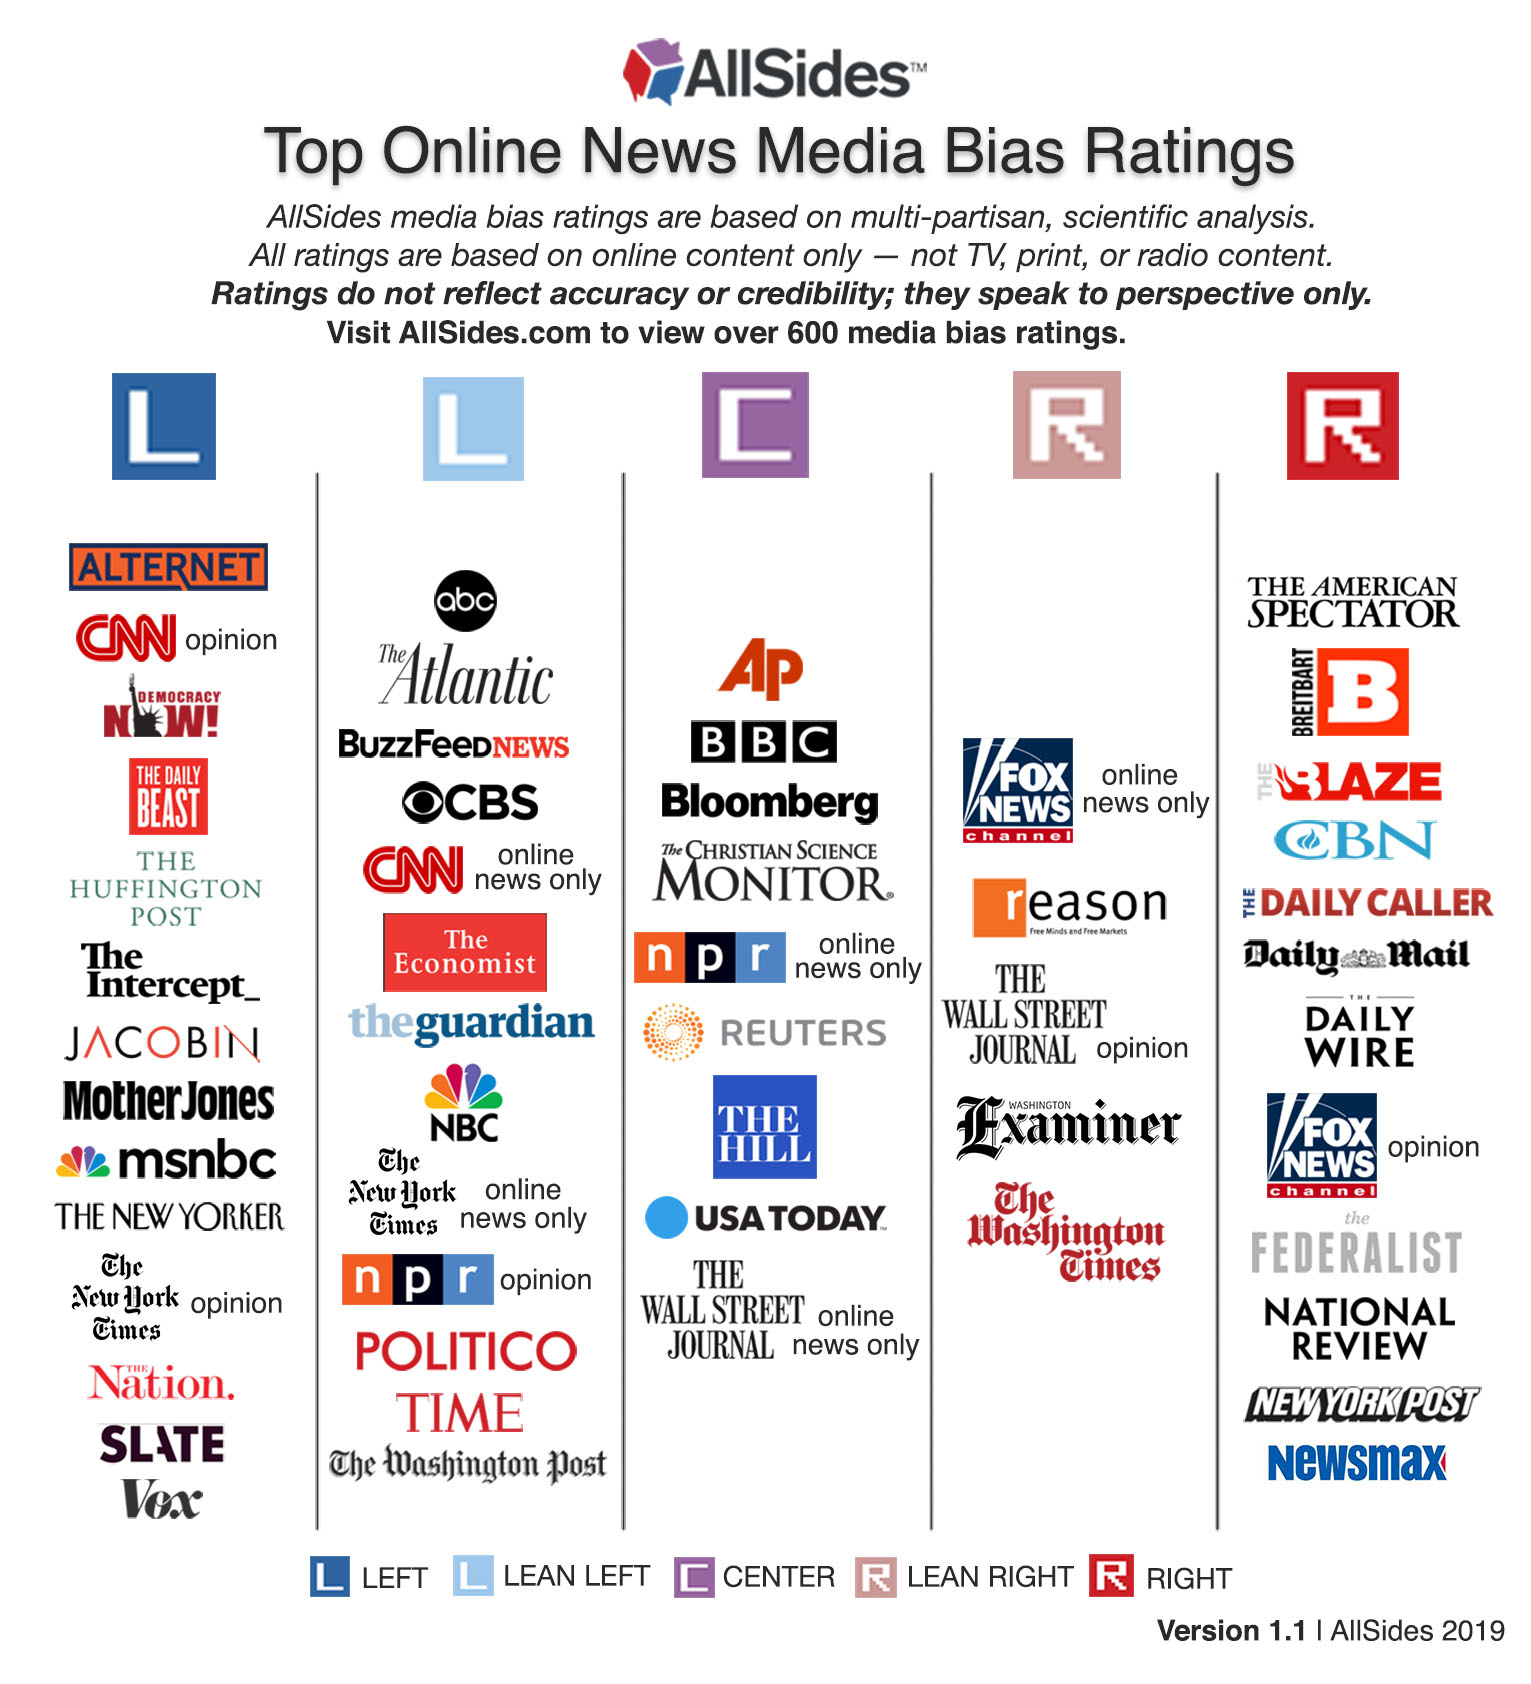
\includegraphics[width=\linewidth]{chapter1/figs/AllSidesMediaBiasChart}
	\caption[An example collection of News-Media sites that have been classified into biases; sourced from AllSides website.]{An example collection of News-Media sites that have been classified into biases; sourced from AllSides website~\cite{gable_media_2019}.}
	\label{fig:allsidesmediabiaschart}
\end{figure}
% </AllSides discussion>



% <sorting organisations>
A list of possible news sources was collected from AllSides on February 1st, 2019. In this collection was an organisation name, political bias, the number of user feedback ratings of the political bias, and, if available, the Twitter handles associated with the organisation. These collected news sources were broad, containing not just news-media organisations but authors, pundits and think tanks. 

We performed the following filtering: a source was only considered if it was a organisation (not an individual), that produced news content of a diverse range of topics. Many news sources were connected to think tanks or opinion groups, and only created news of a single topic or campaign. Further, if a news-media organisation has no Twitter account or had less than 10,000 followers it was removed from the pool. This mainly removed inactive organisations and local news organisations from small rural towns. 

Finally, a single source was removed as it was not in English (\emph{@univision}), and a single source (\emph{@theMRC}) was removed as its content was a subset of its sister site, CNSNews.  The result of this filtering process is 170 news-media organisations with associated Twitter accounts and categorised political biases.  A list of all news-media organisations under analysis can be seen in \autoref{sec:app_accounts} and all removed sources and the removal justification can be seen in \autoref{tab:app_removed_accounts}.
% </sorting organisations>

\subsubsection{Collection}
%  <Twitter collection>
Using the Twitter user handles associated with each news-media organisation, the history of all tweets for each account was collected using the Twitter application programming interface (API)\footnote{\url{https://developer.Twitter.com/en/docs}} and web-scraping tools\footnote{\url{https://github.com/twintproject/twint}}. Of interest in this work are the tweets each news organisation made between January 1st, 2019 to January 1st, 2020, which was the largest practical time-frame possible for analysis during this research project given data collection constraints. 

Over this period major news-media organisations tweeted pieces of news multiple times throughout the day. The manner in which each organisation does this can differ and no standard format is used. The tweets often come in the form of a single line description of an article, alongside a link to the article on the news-media organisation's website. The primary purpose of using social media sites to post these stories is to drive traffic to the organisation's website where they can earn revenue from ad impressions. As such, the format of such news tweets summarises core concepts from articles and frames them in their most essential and appealing way; often they are trying to create so-called `click-bait'~\cite{potthastCrowdsourcingLargeCorpus2018} but even standard reporting is often summarised in a clear tweet-length summary. This format is desirable for our work as we want to explore how the language news-media organisations use to appeal to consumers differs between organisations.

% breaking news
Twitter also serves as a tool for breaking news. The modern 24 hour news cycle has had many effects on journalism, including a pressure to produce breaking news at a lightning fast pace. The use of social media as a near instant tool for global public communication means that often no time is wasted in publishing a story, potentially while it is unfolding. Indeed, research has explored Twitter's role in breaking news in the cases of the 2011 UK summer riots~\cite{vis_Twitter_2013} through providing real time updates over the four days, and in the case of the death of Osama Bin Laden in 2011~\cite{hu_breaking_2012}, where the news was leaked and spread virally through social media before any news-media organisations could fully verify and publish stories on the claim. %
This rapid information exchange can prove dangerous, as in the case of the 2013 Boston Marathon bombing~\cite{starbird_rumors_2014}, where 29\% of the most viral content on Twitter was rumours and fake content~\cite{gupta_100_2013}.
% boston marathon
% These breaking news stories are sometimes, but not always, preceded by expressions such as ``\emph{Breaking News:}''. The inconsistent use of such a preamble can present challenge in our analysis of language moving forward, an \todo{will be explored more in this section}.
%  </Twitter collection>

\subsubsection{Account removal}
% <removal of inactive Twitter accounts>
Using this collection method a total of 3,221,769 tweets were collected from the 170 news-media organisation official Twitter accounts in the 2019 calendar year. This represents an average of above 50 tweets per day for each news organisation. However, the activity level and consistency of output vary greatly between organisations. \autoref{fig:data_cleaning_average_tweet_activity} shows the distribution of average daily number of tweets for each news-media organisations, showing that some news organisations produce very little content on average. This can be explained through two mechanisms.

\begin{figure}[!htbp]
	\centering
	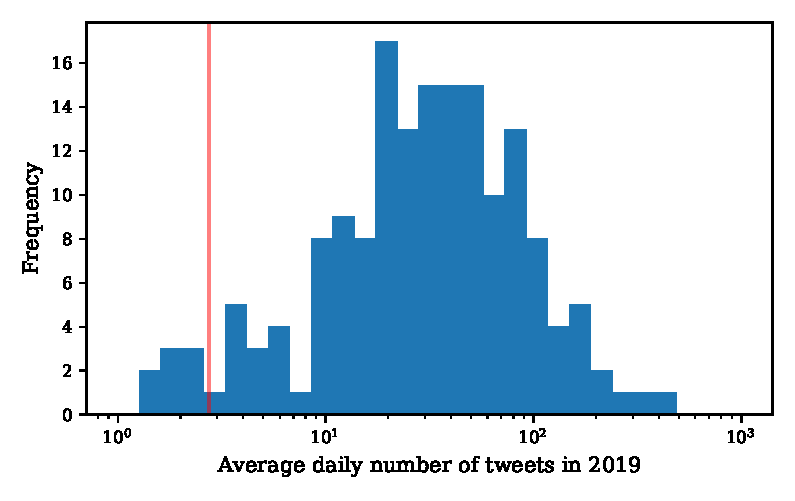
\includegraphics{chapter1/figs/averagetweetactivity}
	\caption{The average number of tweets produced each day during the 2019 calendar year for all 170 news-media organisations. The red line is the chosen threshold of 1000 tweets in the year, an average of 2.74 tweets per day.}
	\label{fig:data_cleaning_average_tweet_activity}
\end{figure}

Firstly, some organisations are not very active on social media. In particular, smaller organisations, which are typically less well resourced, place a lower priority on social media posting. This lower tweet volume presents a challenge for this work. In particular, the use of the non-parametric entropy estimator in \autoref{ch:crossentropy} requires a substantial amount of text to converge. Hence, organisations that produced less than 1000 tweets in 2019 were removed from further consideration. This removed a total of 11 news-media organisations, listed in  \autoref{tab:data_removed_low_tweet_counts}.


\begin{table}[!htbp]
	\centering
	\begin{tabular}{llr}
		\toprule
		News-media Organisation &    Bias  &  Number of tweets in 2019\\
		\midrule
		RealClearPolitics &      Center &  532 \\
		IJR  &  Lean Right &  777 \\
		WND News &         Right &  709 \\
		PRI &                Center &  346 \\
		EurekAlert! &            Center &  610 \\
		FAIR &     Center &  697 \\
		Crowdpac &            Center &  521 \\
		Inside Philanthropy &        Center &  781 \\
		Diplomatic Courier &         Center &  750 \\
		Peacock Panache &          Left &  198 \\
		Independent Voter &            Center &  303 \\
		\bottomrule
	\end{tabular}
\caption{Table of news-media organisations that were removed from data due to a low number of tweets in the 2019 calendar year.}
\label{tab:data_removed_low_tweet_counts}
\end{table}

Secondly, five news-media organisations, for reasons unknown, had large periods of time in which they did not post any tweets. These periods of time, spanning a few months, present key challenges to our investigation. 
Time is an important aspect of news, and this aspect is incorporated into our entropy estimation tools in \autoref{ch:crossentropy}. As such, news organisations that take long breaks will not have fair information theoretic comparisons. These five organisations, listed in \autoref{tab:data_removed_inactive_period} were removed from further analysis.

\begin{table}[!htbp]
	\centering
	\begin{tabular}{ll}
		\toprule
		News-media Organisation &    Bias \\
		\midrule
		American Thinker  &      Right \\
		Pacific Standard &  Lean Left \\
		Philly.com  &  Lean Left \\
		Splinter &       Left \\
		ThinkProgress  &       Left \\
		\bottomrule
	\end{tabular}
	\caption{Table of news-media organisations that were removed from data due to long periods of inactivity.}
	\label{tab:data_removed_inactive_period}
\end{table}


We examined the daily activity of each news-media organisation. An activity curve for the \emph{New York Times} can be seen in \autoref{fig:nytimes_and_tweets_by_weekday}(a). 
A clear weekly trend where tweet activity is decreased during the weekends is seen for most news-media organisations as exemplified when all news-media organisation tweets are aggregated in \autoref{fig:nytimes_and_tweets_by_weekday}(b). Further, many news-media organisations have distinct spikes at key points during the year. These spikes indicate an organisation is covering a rapidly-evolving, breaking news story, or responding to major changes in discourse through the day. These are interesting and important features in the data; the full collection of figures containing the daily activity levels of all included organisations can be seen in \autoref{app:activity}.

\begin{figure}[!htbp]
	\centering
	% \begin{subfigure}[t]{\textwidth}
	% 	\centering
	% 	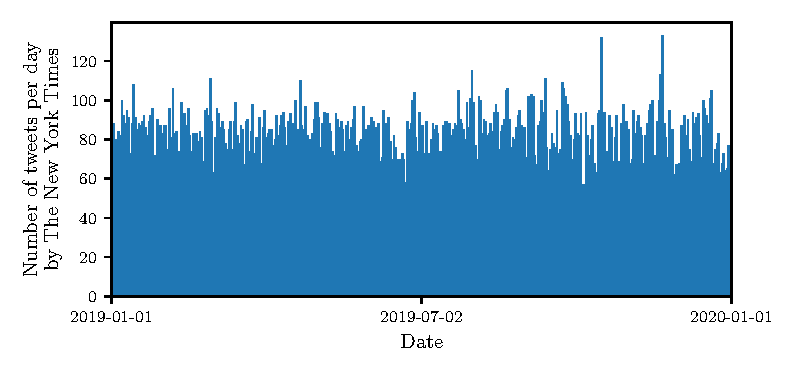
\includegraphics{chapter1/figs/tweet_times_nytimes.pdf}
	% 	\caption{}
	% 	\label{fig:data_newyorktime_activity}
	% \end{subfigure} 
	% \begin{subfigure}[t]{\textwidth}
	% 	\centering
	% 	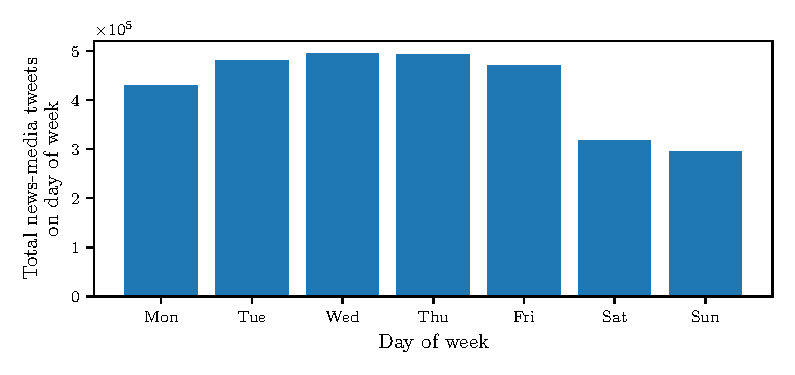
\includegraphics{chapter1/figs/tweet_by_weekday.pdf}
	% 	\caption{}
	% 	\label{fig:tweets_by_weekday}
	% \end{subfigure}
	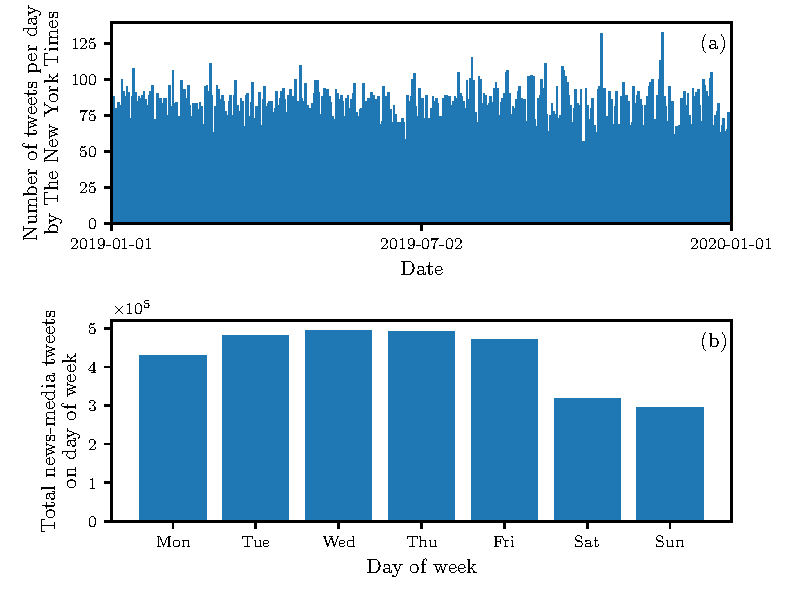
\includegraphics{chapter1/figs/nytimes_day_of_week_merge.pdf}
	\caption{News-media Twitter activity in 2019. (a) is activity for \emph{The New York Times} (account handle \emph{@nytimes}) which is the most followed news-media account with 44,800,317 followers and 31,029 tweets in 2019. Activity figures for other organisations are available in \autoref{app:activity}. (b) shows the total tweet counts by day of week the tweet was posted. A clear weekend reduction in content can be seen.}\label{fig:nytimes_and_tweets_by_weekday}
\end{figure}

% </removal of inactive Twitter accounts>

\subsubsection{Account analysis}
% <metadata>
After filtering we are left with 154 news-media organisations with complete data for the 2019 calendar year. %
These organisations average 52.97 tweets per day, with a total of 2,977,980 tweets.
% Of these organisations the bias distribution is still somewhat representative of social media. \ts{find a source that discusses why left wing is more popular on social media.} 
There are 73 organisations in the left half of the bias spectrum, 44 in the centre and 37 on the right (\autoref{fig:data_number_of_bias_organisations}). This distribution, although shifted towards the left, still provides sufficient samples of bias to explore further.

\begin{table}[!htbp]
	\centering
	\begin{tabular}{lr}
		\toprule
		Bias &   Number of Organisations \\
		\midrule
		{\color{Left} Left }&  31 \\
		{\color{LeanLeft} Lean Left }&  42 \\
		{\color{Center} Center }&  44 \\
		{\color{LeanRight} Lean Right }&  16 \\
		{\color{Right} Right }&  21 \\
		\bottomrule
	\end{tabular}
	\caption{The number of news-media organisations in each political bias classification in our data.}
	\label{fig:data_number_of_bias_organisations}
\end{table}

The news-media Twitter accounts also provide metadata about each organisation. Two useful pieces of metadata are the geographic location, and the number of followers on Twitter.

% location data
The Twitter account of each news-media organisation can elect to provide a free text `location'. In some cases this option can be used for other purposes, such for self promotion (\emph{e.g.} the \emph{New York Daily} states its location as `\texttt{New York City  /  fb.com/nydailynews}') and many organisations elected to leave the field blank. 
Of the organisations with text, locations can be difficult to disambiguate and compare. We therefore classified locations manually in \autoref{tab:data_locations}. Where multiple cities or locations are given, the largest possible inclusion was taken. For example `\texttt{New York and the World}' would become `Worldwide' in our classification, as would `\texttt{NYC, London, Paris, Hong Kong}'. There is a notable U.S focus to the data, as is expected using a U.S. based bias rating tool.

\begin{table}[!htbp]
	\centering
	\begin{tabular}{lr}
		\toprule
		Location &  Counts \\
		\midrule
		New York &      34 \\
		Washington, D.C. &      20 \\
		California &      11 \\
		Other US City &      44 \\
		General US &       8 \\
		Worldwide &       6 \\
		United Kingdom &       5 \\
		Qatar &       1 \\
		Pakistan &       1 \\
		Korea  &       1 \\
		Unspecified or Unclear &      43 \\
		\bottomrule
	\end{tabular}
	\caption{The aggregated self-defined locations of news-media organisations according to their Twitter account metadata. }
	\label{tab:data_locations}
\end{table}

% follower distributions
The number of followers a news-media organisation has on Twitter is an important metric, as it is a proxy for the `reach' of the account.

The most followed organisation in the dataset was the \emph{New York Times} with 44,800,317 accounts following it at the time of collection on the 13th January 2020. The least-followed account was \emph{CalMatters} with 15,069 followers. Interestingly, in addition to being more numerous, the follower counts were slightly higher for left biased organisations than for the right.  This is shown via the followers distributions for each bias in \autoref{fig:data_number_of_follow_by_bias_raincloud}, which is indicative of the larger trend in social media of slightly left-leaning demographics~\cite{mellonTwitterFacebookAre2017}.

\begin{figure}[!htbp]
	\centering
	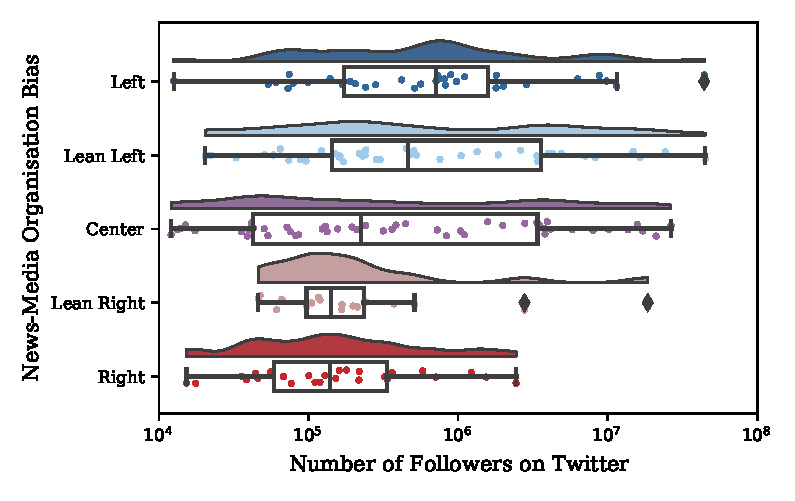
\includegraphics[width=\textwidth]{chapter1/figs/number_of_follow_by_bias_raincloud}
	\caption{Number of followers on Twitter of news-media organisations included in the data grouped according to political bias assigned by AllSides. The full range of political spectrum is represented in the data, with left leaning organisations having a higher average number of followers. }
	\label{fig:data_number_of_follow_by_bias_raincloud}
\end{figure}
% </metadata>

\subsection{Tokenization}

We process the 2,977,980 tweets from filtered dataset into an array of words. As discussed in \autoref{sec:tokenization}, the process of tokenization is applied to each string independently.

The TweetTokenizer\footnote{\url{www.nltk.org/api/nltk.tokenize}} from the Natural Language Toolkit (nltk) in Python is used. This built-in tokenizer is specially designed for tweet-style strings and bundles several useful features.

For each tweet, four steps are applied:
\begin{enumerate}
	\item Twitter account handles, which appear in the form `@account\_name', are removed. Across all accounts, these handles make up 0.88\% of the tokens. While some handles are contextual references, many are reference to piece authors. In the case of the \emph{Los Angeles Times}, 69\% of the references were to its own Twitter account. In general, these handles usually add uninformative differentiation between each organisation's description of the news, and make matching sub-sequences of tokens harder.
	\item Any sequence of a character that repeats more than three times is reduced to a maximum of 3. This has the effect of standardising text of similar meanings a common form, such as `waaaaayyyy' and `waaayyyyy' to `waaayyy'. In doing so, this reduction makes matches between these tokens far more likely.
	\item All URLs included in the text are removed. These URLs are almost always a link to an organisations own story associated with the tweet context. Many organisation's have multiple domains or sister-sites making these hard to isolate without removing all URLs.  
	\item The string is converted to lower-case and split at each white-space, giving an array of individual words. This creates the sequence of tokens that can be most easily compared between organisations.
\end{enumerate}

These steps are applied uniformly across the corpus to identify the flow of linguistic structure within news. In order to achieve this, we need to standardise the text to the most common possible format, such that text of similar phrasing and meaning will be matched between sources. These tokenization and text cleaning steps allow for these similarities to be expressed.


\subsubsection{Vocabulary sizes}\label{sec:vocabsizes}

With the tweets of each Twitter account tokenized, we can begin to explore the vocabulary sizes. The vocabulary size is the number of unique tokens that exist in the collection of all tweets from a news-media organisation, as introduced in \autoref{sec:background_vocab_sizes}. \autoref{fig:data_vocabvsactivity} shows the strong relationship between the amount of tweets produced and the number of unique words, with diminishing increases to vocabulary as new tweets are added. This relationship follows the Herdan–Heaps law \cite{herdan1960type, heaps_law_1978} which states that the vocabulary size, $V$ is distributed $V \sim N^{\beta}$ with $0 < \beta < 1$ and token count $N$. This is an important law that highlights that for any given Twitter account we expect a larger number of tweets will produce a larger vocabulary size.

Of further interest is how each organisation deviates from this law. The ratio of vocabulary size to number of tweets provides a first glimpse into the level of complexity in the language for each news-media organisation. Accounts that have a more specific focus/domain, such as political focused news (\emph{e.g.} \emph{The Hill}), increase their vocabulary at a slower rate as new tweets are added due to the consistently repeating domain specific words. In contrast, an account such as the \emph{The Guardian} produces a diverse array of content, and hence has a larger vocabulary size in contrast to its output.

We see the extreme variance in tweet activity reflected in the distribution of vocabulary size. The vocabulary sizes span from 2,976 unique tokens (\emph{ScienceDaily}) to 40,824 (\emph{The Guardian}). 

This presents a key challenge for this work. We need to find information flows between news-media organisations that can have content corpora that differ in size by two orders of magnitude, and vocabulary sizes that can differ by up to one. This can exacerbate the problems already presented by natural language, and informs the need to normalise flows in later sections.


\begin{figure}[!htbp]
\centering
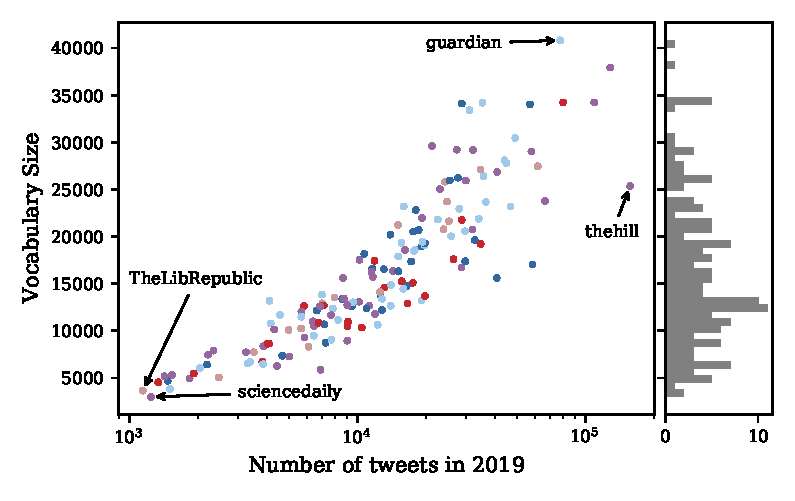
\includegraphics{chapter1/figs/vocab_vs_activity.pdf}
\caption{Vocabulary size from all tweets produced in 2019 for each news-media Twitter account and the total number of tweets produced.}\label{fig:data_vocabvsactivity}
\end{figure}

\subsection{Rank frequency distribution of vocabulary}\label{sec:zipf_fit}

In the remainder of this work we will often use this tokenized corpus of news-media tweets for our analysis. However, in some case we will want to generate synthetic text that has similar properties to our data here. As discussed in \autoref{sec:textgeneration}, we draw i.i.d. from a Zipf distribution to simulate such text. In order to match the properties of the data as best as possible, we fit a Zipf distribution to the data as show in \autoref{fig:data:fitted_zipf}. To extract the fitted scaling parameter of a Zipf distribution, we can fit a linear line to the log of each words frequency with the log of its frequency rank, in the corpus of all tweets. This fitting is meant to be approximate, as it is only used to inform the general range of Zipf law distributions used later, and the fitting of power-laws is often overdone~\cite{broidoScalefreeNetworksAre2019}. 

As has been seen in other corpora~\cite{williams_text_2015,naranan1998models, gerlach2013stochastic}, the rank-frequency distribution shows two different scaling regimes, where common words scale with $\alpha\approx 0.8$ and uncommon words scale with a much higher $\alpha \approx 2$, with an overall scaling parameter of $\alpha=1.2$. Later in thesis this we will use a variety of values for $\alpha$, usually in the range between $0.5$ and $2$ to account for both the variability between organisations and between scaling regimes. In should be noted that in each generation process herein only a single scaling regime is used, a shortcoming of our generation approach.


\begin{figure}[!htbp]
\centering
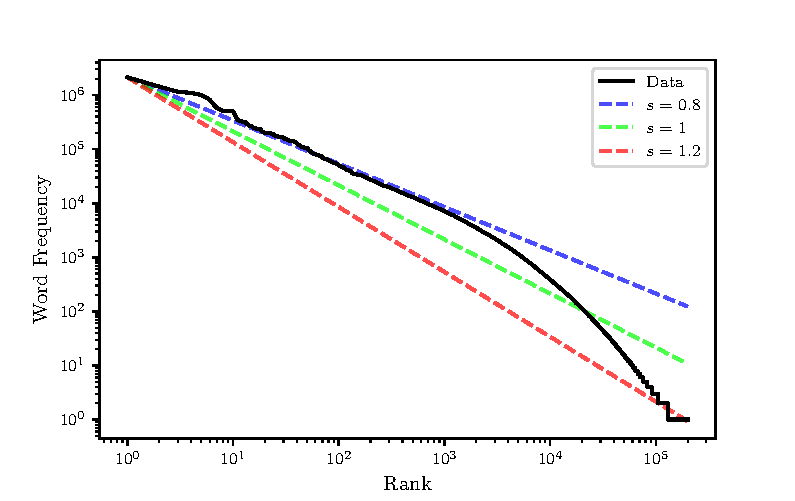
\includegraphics{chapter1/figs/fitted_zipf.pdf}
\caption{Word frequency of tokens in the corpus of all tweets produced by all news-media organisations compared the rank of the tokens by frequency. Zipf law distributions are also shown for varying scaling parameters, $\alpha$. \label{fig:data:fitted_zipf}}
\end{figure} 


Having now collected, cleaned, and performed a basic analysis of the data, we will now use it for two key purposes. Firstly, the development of the entropy estimation tools in \autoref{ch:crossentropy} and information flow measures in \autoref{ch:quotermodel} will use this dataset -- and the synthetic generation of text motivated by it -- to validate the techniques as reliable tools of information flow extraction. We then apply these tools to the data to produce a network, the analysis of which is discussed in \autoref{ch:ranking}.


%\the\textwidth
%
%% somewhere maybe summary
%60054638 words

%!TEX root = ../thesis.tex
\chapter{Entropy rate estimation}\label{ch:crossentropy}

\epigraph{\em ``Semantic aspects of communication are irrelevant to the engineering problem.''}{Claude Shannon, {\em A Mathematical Theory of Communication}, 1948}

Extracting information flows is a problem deeply rooted in information theory. To examine these flows requires tools to quantify and measure this information in the form of natural language. As discussed in \autoref{ch:background}, the words used to construct language have no qualitative meaning in the context of the numerical analysis. Thus the tools are comparative in nature. Indeed, information theory has been used extensively to compare properties of information in language~\cite{shannon_prediction_1951,cover_convergent_1978,brown_estimate_1992}. 

In this chapter, we extend this philosophy in two key ways. We introduce a non-parametric entropy rate estimator and check its assumptions using real data. We then generalise this entropy rate to a cross entropy rate, developing a tool for analysing information flows. These new estimators are then made into a high speed open-source package which is applied to our news data. 

\section{Entropy rate estimation}

Recall \autoref{def:entropyrate} of the entropy rate of a stochastic process. While a useful theoretical tool, this can be very difficult to compute, requiring knowledge of the joint entropy for an infinite set of realisations.

To overcome this, we seek a way to estimate the entropy of the process from a known sequence of data. In 1998 Kontoyiannis \emph{et al.}~\cite{kontoyiannis_nonparametric_1998} proved the convergence of a non-parametric entropy estimator for stationary processes.

\begin{definition}[Kontoyiannis Entropy Rate] \label{def:Kontoyiannis}
	For a discrete valued stochastic process $\mathcal{X} = \{X_i\}_{i=0}^N$, with $N$ realisations, the entropy rate is given by,
	\begin{equation}\label{eq:entropy:Kontoyiannisdef}
		H(\mathcal{X}) = \lim_{N\to \infty}\frac{N \log N }{\sum_{i=0}^N \Lambda_{i} },
	\end{equation}
	where  $\Lambda_{i}$ is the length of the shortest subsequence starting at position $i$ that does not appear as a contiguous subsequence in the previous $i$ symbols, $X_{0}^{i} = \{X_k\}_{k=0}^i $. This can also be obtained by adding 1 to the longest match-length, 
	 \begin{equation}\label{eq:entropy:lambda}
	  \Lambda_{i}=1+\max \left\{\ell: X_{i}^{i+\ell}=X_{j}^{j+\ell}, 0 \leq j \leq N-i, 0 \leq \ell \leq N - i - j \right\}.
	 \end{equation}
\end{definition}

%<lit review>
This idea of using matched sub-sequences of text draws from the original work by Lempel and Ziv~\cite{ziv_universal_1977} in compression algorithms. These algorithms attempt to compress a sequence down into the smallest possible representation, which at perfect efficiency would be the entropy, $H$. However these universal coding algorithms have no universal rate of convergence~\cite{shields_universal_1993, shields_universal_1995} and in practice other approaches are often employed, tailored to the specific application at hand.

The idea of an entropy estimator based on match lengths was originally put forward by Grassberger~\cite{grassberger_estimating_1989} and proved consistent for independent and identically distributed (i.i.d.) processes and mixing Markov chains~\cite{shields_entropy_1992}, stationary processes~\cite{kontoyiannis_prefixes_1994} and more generally for random fields~\cite{quas_entropy_1999}.


Wyner and Ziv~\cite{wyner_asymptotic_1989} showed that for every ergodic process the match length $\Lambda_{n}$ grows like $\frac{\log{n}}{H}$ in probability.  Extending from this notion Kontoyiannis \emph{et al.} showed the convergence of \autoref{eq:entropy:Kontoyiannisdef} in stationary ergodic processes using the match-length $ \Lambda_{i}$. This match-length in \autoref{eq:entropy:lambda} can be seen as the length of the next phrase to be encoded in the sliding-window Lempel–Ziv algorithm.

%<match lengths>
Conceptually, this match-length is simple. \autoref{fig:entropy:matchlength} shows the calculation of two match-lengths at different time points of a line from Green Eggs and Ham by Doctor Seuss. At each index $i$, the elements immediately proceeding ($i, i+1, i+2, \dots$) are compared to the history of elements before $i$. The matches of length $k$ are found such that the elements from $j$ to $j+k$ perfectly match the elements from $i$ to $i+k$, for any $j<i$ where $k$ is then maximised. This search only considers the length of the match, regardless of its location in the history. 

\begin{figure}[!htbp]
	\centering
	\includestandalone[width=\textwidth]{chapter2/figs/tikz/lambda_count}
	\caption{An example calculation of the match-length based $\Lambda_i$ applied to a words in a line of text from Green Eggs and Ham by Doctor Seuss. The {\color{blue}blue texts} are words which have been matched from past to the future. As $i$ changes, the longest match length possible starting at index $i$ will change.\label{fig:entropy:matchlength}} 
\end{figure}
%</match lengths>

Even before its formalisation by Kontoyiannis \emph{et al.}, similar estimators had appeared in the literature applied to experimental data to determine the entropy rates of processes~\cite{chen_using_1993, chen_fast_1995, farach_entropy_1995, juola_what_1997}.
%</lit review>

% Final note
Moving forward we will assume any any discussion of the \emph{entropy rate} of a single process is assumed to be the \emph{Kontoyiannis entropy rate} of that process, unless otherwise stated.


% ASSSUMPTIONS
\section{Assumptions of entropy rate estimation}

The proof of convergence of this entropy rate places some limits on the process of investigation. In particular, three assumptions are made for convergence: ergodicity, stationarity and the Doeblin Condition (DC).

The Doeblin Condition is a reasonably weak condition, but is fundamental in the proof of the convergence. Simply put, the DC requires that after an arbitrary $r$ time steps, every state is possible again with positive probability~\cite{kontoyiannis_prefixes_1994}. More formally, the definition is as follows.

\begin{definition}[Doeblin Condition (DC)]
	There exists an integer $r\geq 1$ and a real number $\beta \in(0,1)$ such that, for all states $x_{0} \in \mathcal{A}$, 
	$$P\left\{X_{0}=x_{0} \mid X_{-\infty}^{-r}\right\} \geq \beta, $$ 
	with probability one. 
\end{definition}

Fortunately, as Kontoyiannis \emph{et al.} themselves state, the DC is ``certainly satisfied by natural languages''~\cite{kontoyiannis_nonparametric_1998}. 

In contrast, the assumptions of ergodicity and stationarity are  harder to confirm. A long-standing assumption of information theory is that natural language can be modelled by a stationary process~\cite{shannon_mathematical_1948, shannon_prediction_1951, cover_elements_2012}. The assumption, while flawed, has a long precedent and we use it again in this work.

Much of the literature including the work of Kontoyiannis assume ergodicity of natural language, however some suggest that language should be modelled by a \emph{strongly nonergodic} stationary process~\cite{debowski_is_2018}. In brief, this contention is founded upon the idea that any given collection of text, such as a book, has a topic containing a small finite subset of words. Which suggests that its text cannot explore the full state space of language. While well founded, our interest is not to look at the entropy rate of the English language as a whole, but rather to look at the entropy rate of individual text streams, which can all explore the state space of news under consideration. As such, the assumptions of ergodicity and stationarity appear justified in the context of the problem.


%<Convergence>
\subsubsection{Convergence}
With the assumptions of the proof addressed, the challenge of entropy rate estimation convergence needs to be examined. The entropy rate defined in \autoref{eq:entropy:Kontoyiannisdef} is based upon an infinite set of data. In reality, we have finite data, and need to examine the convergence of a modified estimator.

\begin{definition}[Kontoyiannis Entropy Rate Estimator] \label{def:Kontoyiannisestimate}
	The Kontoyiannis Entropy Rate in \autoref{def:Kontoyiannis} can be estimated on a finite stochastic process $\mathcal{X} = \{X_i\}$, with $N$ realisations, by
	\begin{equation}\label{eq:estimate}
		\hat{h} = \frac{N \log N }{\sum_{i=0}^n \Lambda_{i} },
	\end{equation}
	where  $\Lambda_{i}$ is, as earlier, the length of the shortest subsequence starting at position $i$ that does not appear as a contiguous subsequence in the previous $i$ symbols $X_{0}^{i}$.
	 \begin{equation}
	  \Lambda_{i}=1+\max \left\{\ell: X_{i}^{i+\ell}=X_{j}^{j+\ell}, 0 \leq j \leq N-i, 0 \leq \ell \leq N - i - j \right\}.
	 \end{equation}
\end{definition}

To examine the convergence of this estimator, a model of language can be used to generate sequences of text, upon which we can estimate the entropy rate.

%<Zipf convergence>
\begin{figure}[!htbp]
\centering
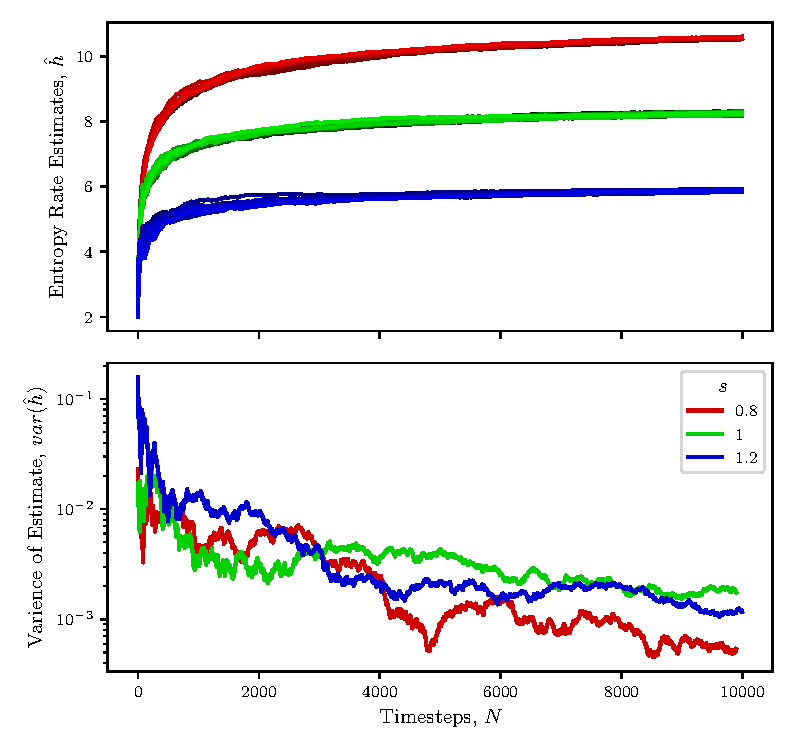
\includegraphics[width=\textwidth]{chapter2/figs/Zipf_entropy_convergence.pdf}
\caption{Convergence of the Kontoyiannis entropy rate estimator on sequences of i.i.d. Zipf distribution realisations with varying Zipf distribution rates, $\alpha$. \label{fig:entropy:zipfconvergence}}
\end{figure}


\autoref{fig:entropy:zipfconvergence} shows the convergence of the estimator for a set of i.i.d. realisations of a Zipf distribution. As discussed in \autoref{sec:textgeneration}, the Zipf distribution is a common tool for generating simple text due to its similarity to the power-law distributions of vocabulary seen in real corpora. The Zipf distribution can be used with a number of scaling parameters, $\alpha$, where larger scaling parameters tighten the distribution, reducing the observed vocabulary size of the sequence and hence the entropy. 

Sequences are generated with 30,000 i.i.d. elements drawn from a Zipf distribution and the entropy rate of estimate of the process is calculated at each timestep between 1 and 30,000 using \autoref{eq:estimate} applied to only the elements before that timestep. Estimates of entropy start very low when few elements are available and rapidly rise as new elements add complexity. Within the first few hundred timesteps entropy estimates can vary between timesteps as new elements are added matching or not-matching previous elements. This is reflected in the high variance between entropies estimates for Zipf process with the same scaling parameter in these early stages. As the number of timesteps included reaches 5000 to 7500 the apparent bias from the asymptotic rate and variance of the estimates are significantly reduced and begin plateauing. 

As more timesteps are added, the estimator continues to converge to the asymptotic entropy and the variance between estimates continues to reduce. High complexity sequences take longer to converge to this entropy, but achieve suitably small levels of bias and variance within 15,000 timesteps even for high entropy sequences. This is an important finding given the speed of calculating these estimates. The algorithm to calculate the match-lengths needed for estimating the entropy is $O(N^3)$ time complexity for the number of included timesteps $N$. As a result, calculations are extremely slow as the number of timesteps gets large. When performing simulations a parsimonious choice of simulation length is advantageous in allowing multiple simulations to be run. Hence, for Zipf distributions a simulation length of 15,000 is deemed sufficient for convergence to the entropy.
%</Zipf convergence>


%<Zipf real entropy>
To confirm the validity of this approach, we can examine the known entropy rate of the Zipf processes. As proved in \autoref{sec:entropyrate}, the entropy rate of an i.i.d. process is simply the entropy of each element. In the case of a Zipf distribution the distribution has entropy\footnote{
	Proof: The probability of a word of rank $k$ being selected from a pool of $V$ elements using scaling parameters $\alpha$ is $(k^\alpha H_{V,\alpha})^{-1}$. Hence, the entropy of each individual element is $\sum_{k=1}^V  (k^\alpha V_{V,\alpha})^{-1} \ln\left( (k^\alpha V_{V,\alpha})^{-1} \right)$. Using $H_{V,\alpha} = \sum_{k=1}^V \frac{1}{k^\alpha}$, this can be rearranged to $\frac{\alpha}{H_{V, \alpha}} \sum_{k=1}^{V} \frac{\ln (k)}{k^{\alpha}}+\ln \left(H_{V, \alpha}\right)$. 
}, 
\begin{equation}
	\frac{s}{H_{V, \alpha}} \sum_{k=1}^{V} \frac{\ln (k)}{k^{\alpha}}+\ln \left(H_{V, \alpha}\right),
\end{equation}
where $H_{V,\alpha}$ is the $V$th generalized harmonic number defined by, 
$$H_{V,\alpha} = \sum_{k=1}^V \frac{1}{k^\alpha},$$
and $V$ is the size of the state space of the Zipf distribution. Many approaches to calculating this entropy use the asymptotic entropy as $V \to \infty$. This draws on the result that $\lim_{V\to \infty} H_{V,s} = \zeta(\alpha)$, where $\zeta$ is the Riemann zeta function. While this asymptotic approach works well for numbers well above 1, the Riemann zeta function diverges to infinity at $\alpha \to 1$. As such, the analytic entropy degenerates as $\alpha \to 1$ and is poorly defined for $\alpha < 1$. In contrast, using a finite choice of $V$ results in well defined processes and entropies for all $\alpha >0$. A choice of $V=199,338$ is made to match the observed total vocabulary size seen in the news-media Twitter data as explored in \autoref{sec:vocabsizes}. For high values of $\alpha$, the two asymptotic and finite entropies are very close (\emph{e.g}, for $\alpha=1.5$ the entropies are 3.18158 and 3.18368 respectively), and only differ significantly as $\alpha$ approaches 1. This finite entropy calculation allows the model to more accurately match the Zipf scaling parameters fitted to real text data, which are often closer to or below~1~\cite{williams_text_2015}.

% <Simulations>
Using simulations of the Zipf process for a variety of values of the scaling parameter $\alpha$, we compare how the estimated entropy rate compares to the `true' entropy rate as calculated above. In \autoref{figs:entropy:convergencetotruth} simulations are run for values of $\alpha$ in the range [0.01, 2] with increments of 0.01. 
High values of $\alpha$ in this range have a progressively lower entropy, as the skewness of the distribution becomes more extreme. This distribution results in a large number of realisations of low rank words creating repeated sequences which lower both the analytic entropy rate and the entropy rate estimate. Values above 2 reduce the entropy rate in vanishingly smaller increments. 

\begin{figure}[!htbp]
\centering
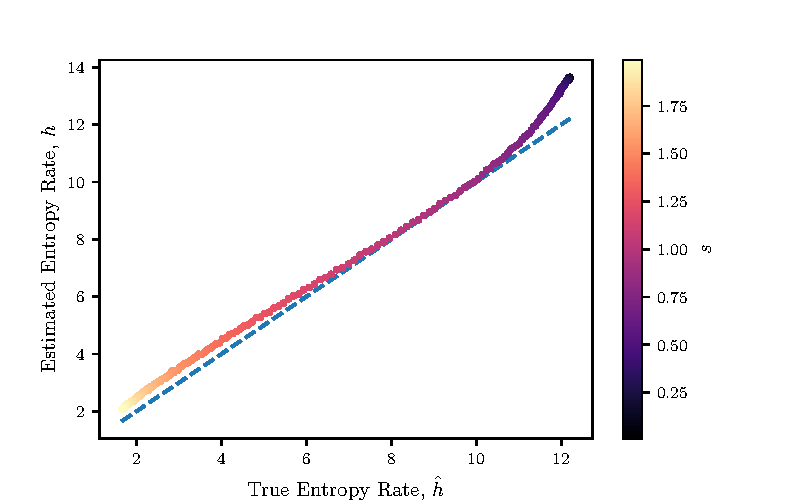
\includegraphics{chapter2/figs/convergence_to_truth.pdf}
\caption{Estimated entropy rates and analytic entropy rates of sequences of 20,000 i.i.d. Zipf distribution random variables with scaling parameter $\alpha$. Dashed line represents the true entropy rate equalling the entropy rate estimate. As values for $\alpha$ approach 0 the high variance of the distributions results in poor estimates due to the finite sample of the Zipf distribution. \label{figs:entropy:convergencetotruth}}
\end{figure}

For values of $\alpha$ between 2 and 0.5, the entropy rate estimate appears to be a rough upper bound on the true entropy rate of the process. This upper bound is only achieved with sufficient lengths of sequences such that the estimator can converge to this upper bound. Indeed, given sufficient length the variance of the estimates on sequences drawn from the same distribution is very low. This is in contrast to the bias of the estimate, which varies with the changing scaling parameter. 

When $\alpha$ becomes lower than 0.5, the Zipf distribution becomes more evenly distributed with reduced skew. This results in a larger probability of low rank word occurrences, producing a process where many words appear very few times. As a result, the finite nature of the sequence results in a entropy rate estimate that grows faster than the true entropy, increasing the bias for these high entropy sequences. 

In general, the convergence of the estimator is sufficient, with a slight caveat: while the estimator convergences to an estimate tightly with very little variance, the bias of the estimate is not constant and varies with the complexity of the sequences. While this finding is itself interesting and warrants future work, the estimator is both consistent and its estimates appear monotonic with the true entropy rate. As such, we will use this estimator to approximate the true entropy rate moving forward, with a cautious eye to the possible effects of this inconsistent bias. 
%</Zipf real entropy>

%<Real data entropy convergence>
To extend from this result, we apply the same approach replacing Zipf distribution generation with text from the news-source Twitter data. 5000 tweets are drawn uniformly from the collection of all tweets from all news-media outlets. These tweets are tokenized and concatenated into a single sequence of natural language text ranging from 85,000 to 90,000 tokens.

Unlike the case of Zipf, we cannot show a true entropy rate for this distribution, as it's unknown, but can demonstrate its convergence.  Each sample has the entropy rate calculated using only the first $N$ tokens, up to the length of 60,000 tokens. \autoref{fig:entropy:realconvergence} shows the clear convergence of the estimator on the real data, approaching an entropy rate of 7.53. As with the Zipf simulations, the variance of the estimated entropy rates of the samples reduces as more tokens are included in the estimate.  The real data takes longer to converge, needing up to 50,000 tokens to achieve a variance of less that $10^{-3}$.

\begin{figure}[!htbp]
\centering
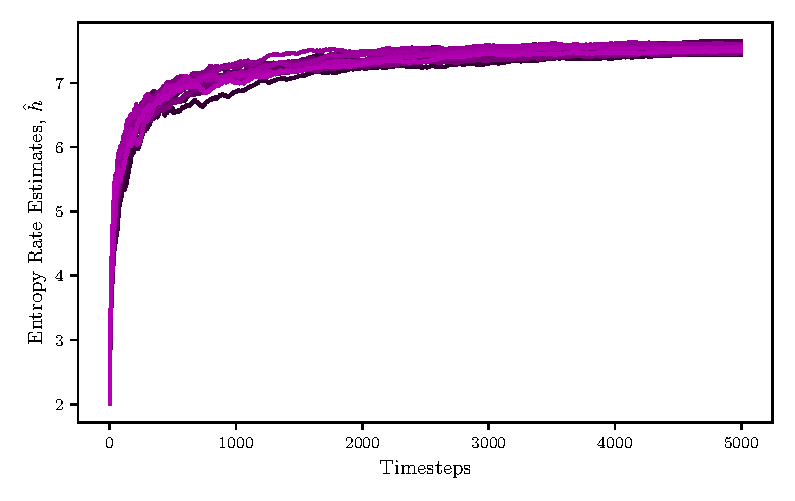
\includegraphics{chapter2/figs/real_entropy_convergence.pdf}
\caption{Convergence of the Kontoyiannis entropy rate estimator on sequences words generated by drawing tweets uniformly without replacement from the pool of all tweets produced by all news-media organisations. Multiple sequences are drawn with most convergence curves overlapping. \label{fig:entropy:realconvergence}}
\end{figure}

%</Real data entropy convergence>

%<Tikz of flow>
\subsubsection{Self entropy rate summary}

\begin{figure}[!htbp]
	\centering
	\includestandalone[width=\textwidth]{chapter2/figs/tikz/self_flow}
	\caption{A conceptual diagram of entropy rate estimation using the Kontoyiannis entropy rate estimation. Tweets shown as blue rectangles are positioned in time and contain textual content. Content proceeding the position \emph{Now} will have snippets of text matched with text from the history of the process, denoted by {\color{orange}orange} and \underline{underlined} text. These text matches are used to calculate $\Lambda_i$ which is used in the entropy estimate. \label{fig:entropy:selfflow}} 
\end{figure}

Before moving away from the entropy rate of a single process, we visualise the how the Kontoyiannis entropy rate estimator works for real data. \autoref{fig:entropy:selfflow} shows a simplified version of the conceptual entropy rate calculation. For a given Twitter user, tweets appear sequentially, separated in time. At any given time, the content of the immediate future of that user's tweets is compared to the entire history of the tweets before that time. This process is then repeated for all possible times in the data. In essence, the calculation of the $\Lambda_i$ is a repeated examination of how much of the immediate complexity at timestep $i$ can be described using the history of the sequence. In total, this estimator provides an average of how many bits are needed to describe the future of this process given its past at any point. 

%% Histogram of self entropy rates ??

%</Tikz of flow>

\section{Cross entropy rate}

To create a notion of information flow, we need to move beyond looking at an individual source in isolation. To do so, we need a tool of comparison between sources rooted in our tools from information theory. We find such a tool in a generalisation to a Kontoyiannis cross entropy rate.

Similar to the extension of entropy, $$H(X) = \sum_{x \in \mathcal{X}} p(x)\log p(x)=-\mathbb{E}[\log P(X)],$$ to cross entropy, $$H(p,q) = \sum_{x \in \mathcal{X}} p(x)\log q(x) = -\mathbb{E}_p[\log q(X)],$$  in \autoref{def:crossentropy}, we can generalise our notion of Kontoyiannis entropy rate from \autoref{def:Kontoyiannis} to a \emph{cross} entropy rate which we will call the Kontoyiannis cross entropy rate. This Kontoyiannis cross entropy rate comes in two forms, a full cross entropy and a time-synced cross entropy.

\begin{definition}[Kontoyiannis Full Cross Entropy Rate]
	The cross entropy rate of a {\color{target} target process} $\mathcal{T}$ coded from a {\color{source} source process} $\mathcal{S}$ can be estimated via,
	\begin{equation}
	H(\mathcal{T} || \mathcal{S})=\frac{N_{\mathcal{T}} \log _{2} N_{\mathcal{S}}}{\sum_{i=1}^{N_{\mathcal{T}}} \Lambda_{i}(\mathcal{T}| \mathcal{S})}
	\end{equation}
	Where $N_{\mathcal{X}}$ is the length of process $\mathcal{X} \in \{\mathcal{T}, \mathcal{S}\}$ and $\Lambda_{i}(\mathcal{T}| \mathcal{S})$ is given by the shortest subsequence starting at position $i$ in the {\color{target}target} $\mathcal{T}$ that does not appear as a contiguous subsequence anywhere in the {\color{source}source} $\mathcal{S}$.
	\begin{equation}
	\Lambda_{i}(\mathcal{T}| \mathcal{S}) = \max \left\{\ell: T_i^{i+\ell}=S_{j}^{j+\ell}, 0 \leq j \leq N_{\mathcal{S}},  0 \leq \ell \leq \min( N_{\mathcal{S}}- j , N_{\mathcal{T}}- i )\right\},
	\end{equation}
	where $T_a^{b}$ and $S_a^b$ are continuous subsequences starting from index $a$ to index $b$ of the {\color{target} target}, $\mathcal{T}$, and  {\color{source} source}, $\mathcal{S}$, processes respectively.
\end{definition}

This approach to cross entropy matches segments of text in the {\color{target}target} to segments of text anywhere in the {\color{source}source} in the same manner that the Kontoyiannis entropy rate matched segments of text in the future of a process from a index, $i$, to the history before the index. In contrast to the entropy rate estimate, which asked how much information was needed on average to \emph{describe the future of a source from its past}, this cross entropy rate estimate is asking how much information is needed on average to \emph{describe the target given full knowledge of the source}. 

\begin{figure}[!htbp]
	\centering
	\includestandalone[width=\textwidth]{chapter2/figs/tikz/unsynced_flow}
	\caption{A conceptual diagram of Kontoyiannis full cross entropy rate estimation. Tweets shown as rectangles are positioned in time for both a target and source, containing textual information. Content in the {\color{source}source} is matched with content in the immediate future of the {\color{target}target} for a given time point, $t$, to calculate match-lengths. This time point is shifted along the {\color{target}target} timeline to average match-lengths and calculate the full cross entropy rate.\label{fig:entropy:unsyncedflow}} 
\end{figure}

This full knowledge over all of the process gives the estimator the `Full' in its title, but presents a impropriety. In the context of our problem, this estimator is cheating by viewing the future of news through the lens of the source process. 

As \autoref{fig:entropy:unsyncedflow} illustrates, the text subsequence match in the target could be drawn from future time points in the source. Restated, the cross entropy rate will, in-part, be describing how much information is needed to encode the future of a piece of target news already knowing the future of the news from another source. While this may be an interesting insight in itself, and could be used in future work to format a notion of information divergence, it doesn't probe the underlying process of \emph{information flow} with which this thesis focuses. 

Rather than looking at the entire lifetime of the source during the matching calculations, we can reduce our search space to the text that occurred in the \emph{past} of the source. To achieve this we use an important piece of our data, the time that tweets occurred. For each word in the target process, $T_i$ has an associated time with it, $t(T_i)$. When matching the future of $\mathcal{T}$, starting from an index $i$, we can reduce the source process, $\mathcal{S}$ to only the words that were themselves tweeted before time $t(T_i)$. 

Put simply, we can alter the Kontoyiannis full cross entropy rate to a time-synced cross entropy rate by replacing the full source process, $\mathcal{S}$, with a time reduced source process $\mathcal{S}_{ \leq t(T_i)}$. This can be seen visually in \autoref{fig:entropy:timesyncedflow} and is formally defined as follows.

\begin{definition}[Kontoyiannis Time-synced Cross Entropy Rate]
	The time-synced cross entropy rate of a {\color{target}target} process $\mathcal{T}$ coded from a {\color{source}source} process $\mathcal{S}$ can be estimated via,
	\begin{equation}
	H(\mathcal{T} || \mathcal{S})=\frac{N_{\mathcal{T}} \log _{2} N_{\mathcal{S}}}{\sum_{i=1}^{N_{\mathcal{T}}} \Lambda_{i}(\mathcal{T}| \mathcal{S}_{\leq t(T_i) } )}
	\end{equation}
	Where $\Lambda_{i}(\mathcal{T}| \mathcal{S}_{\leq t(T_i) })$ is given by the shortest subsequence starting at position $i$ in {\color{target}target} $\mathcal{T}$ that does not appear as a contiguous subsequence in the time reduced {\color{source}source} $\mathcal{S}_{\leq t(T_i) }$ where,
	\begin{equation}
	\mathcal{S}_{\leq t(T_i) } = \{S_j | t(S_j) \leq t(T_i),  \forall i \}.
	\end{equation}
	Which gives,
	\begin{align*}
	\Lambda_{i}(\mathcal{T}| \mathcal{S}_{\leq t(T_i)}) = \max \{\ell: T_i^{i+\ell}=S_{j}^{j+\ell}, 0 \leq j \leq N_{\mathcal{S}},  \\  0 \leq \ell \leq \min( N_{\mathcal{S}}- j , N_{\mathcal{T}}- i ) \},
	\end{align*}
	where $T_a^{b}$ and $S_a^b$ are continuous subsequences starting from index $a$ to index $b$ of the {\color{target} target}, $\mathcal{T}$ process, and the time reduced {\color{source} source}, $\mathcal{S}_{\leq t(T_i)}$, respectively.
\end{definition}

\begin{figure}[!htbp]
	\centering
	\includestandalone[width=\textwidth]{chapter2/figs/tikz/timesynced_flow}
	\caption{A conceptual diagram of Kontoyiannis time-synced cross entropy rate estimation. Tweets shown as rectangles are positioned in time for both a target and source, containing textual information. Content in the {\color{source}source} that occurs before time $t$ is matched with content in the immediate future of the {\color{target}target} from $t$ to calculate match-lengths. This time point is shifted along the {\color{target}target} timeline to average match-lengths and calculate the time-synced cross entropy rate.\label{fig:entropy:timesyncedflow}} 
\end{figure}


% Informantion flow idea
This time-synced cross entropy rate is testing not just the differences in the language processes of the source and target, but also measuring what information in the target is present in the source's history. This is an important distinction, as it allows us to probe a very important aspect of our data, namely, the time in which news is created. 

If a piece of information appears earlier in the source than in the target, it will be detected during the match length search, resulting in a lower entropy. This is to say, in the context of news, if the {\color{source}source} breaks a story first, \emph{less} information is required to describe the subsequent news output from the {\color{target}target}. 

Conversely, if a {\color{target}target} produces a piece of information before the {\color{source}source}, then that information will not appear in the history of the time-synced source during the match-length search. This will result in lower values of $\Lambda_i$ for that piece of information, which raises the cross entropy rate.

From this, we can find that, on average, if a {\color{source}source} produces information earlier than a {\color{target}target}, the cross entropy rate, $\hat{h}(\mathcal{T} || \mathcal{S})$, will be lower than if the {\color{target}target} produces information earlier than the {\color{source}source}. This method of examining who produces information first can be extended into a notion of \emph{information flow}, a discussion we will leave for \autoref{ch:quotermodel}.


\subsection{Validating the assumptions of cross entropy estimation}

To validate these new cross entropy rate estimators a similar process is performed as with the entropy rate. Fortunately, many of the assumptions transfer over directly.

In the case of ergodicity, stationarity and the Doeblin Condition, all three are properties of the process under investigation, which we argued above are well founded. We introduce an additional condition on the processes for the sake of cross entropy rates, namely that the processes have the same state space. This additional condition extends the earlier conditions to apply jointly between both the source and target processes. While not all news-media organisations will have the same realisations of words in their corpus, the processes could be reasonably thought to have the same state space, as all processes are using English and discussing similar topics.

This then leads naturally to the next question of convergence. Following a similar process of uniform withdrawals from a distribution will result in functionally similar convergence to the entropy rate above. Indeed, this can be seen in \autoref{fig:entropy:realcrossconvergence}, where tweets are draw uniformly from the pool of all tweets and cross entropy rates are calculated on the resulting sequences. Here, the cross entropy rate is denoted $\hat{h}_{\times}$ to distinguish from the entropy rate estimates $\hat{h}$. This figure is, as expected, functionally similar to \autoref{fig:entropy:realconvergence} from the entropy rate section above. This cross entropy rate calculation is fundamentally no different from the original entropy rate calculation with these sequences, as a randomly selected history of another process is just a useful and a randomly selected history the original process when both draw from the same distribution.


\begin{figure}[!htbp]
	\centering
	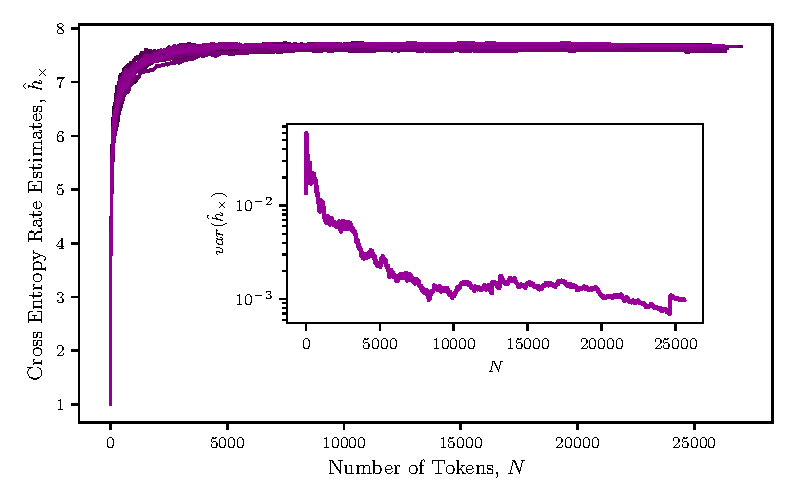
\includegraphics{chapter2/figs/cross_real_entropy_convergence}
	\caption{Convergence of the Kontoyiannis time-synced cross entropy rate estimator on pairs of sequences independently generated by drawing tweets uniformly without replacement from the pool of all tweets produced by all news-media organisations.} \label{fig:entropy:realcrossconvergence}
\end{figure}

A more nuanced investigation of the cross entropy convergence emerges when we utilise processes with \emph{different} distributions. \autoref{fig:entropy:zipfcrossconvergence} does exactly this. Using pairs of scaling parameters for different Zipf distributions, simulations of 30,000 long i.i.d.~ processes are made with separate target and source processes. The cross entropies rates are then estimated across these pairs. When the scaling parameters are equal, $\alpha_{source}=\alpha_{target}$, we observe the same entropy and convergence pattern as we would for a single i.i.d. process with that distribution. 

\begin{figure}[!htbp]
	\centering
	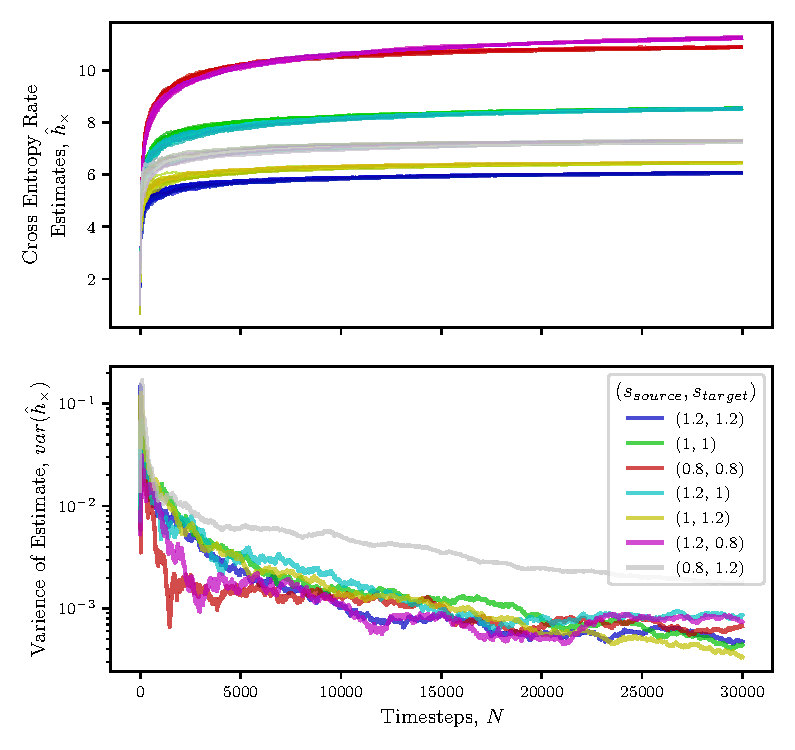
\includegraphics{chapter2/figs/cross_Zipf_entropy_convergence.pdf}
	\caption{Convergence of the Kontoyiannis time-synced cross entropy rate estimator on pairs sequences of i.i.d. Zipf distribution realisations with varying pairs of Zipf distribution rates, $\alpha_{source}$ and $\alpha_{target}$. } \label{fig:entropy:zipfcrossconvergence}
\end{figure}

When $\alpha_{source} \neq \alpha_{target}$ the entropy rates vary, and are not always similar to the entropy rate of the target or the source. Most cross entropy rates converge at a similar pace to the entropy rates above, although large deviations between distributions can reduce this rate of convergence. In particular when the source has significantly higher complexity than the target, as in the case of $(\alpha_{source}, \alpha_{target}) = (0.8,1.2)$, the entropy takes much longer to converge as it requires longer for common patterns to occur in the high complexity source for sequence matching. % talk more





\subsection{Predictability}
With the Kontoyiannis cross entropy rate estimator converging, we also want to generalise the notion of maximal predictability.
We introduced maximal predictability, $\pi^{max}(S,V)$,  in \autoref{def:maximialpredictability} as it is a robust way of determining an upper bound on how well the future of a process could be predicted from its past. The use of the state space size, allows for normalisation of the entropy rate when state spaces are large. The state space size will be represented as $V$ as the state space of language is the vocabulary.

In order to generalise this notion of maximal predictability, we need to identify the two replacements for the inputs. The replacement for entropy rate is trivially the cross entropy rate, but the choice of state space size is more nuanced. Three choices are possible, the state space of the source, $V_{source}$, the target, $V_{target}$, and the union of the state spaces $V_{union}$. 

The original motivation behind the maximal predictability is to normalised the entropy by \emph{how complex the system we are trying to predict is}. This complexity is a property of the target. While a complex source does change how well the target can be predicted, it is the property of the target that needs to be controlled for. As such, the choice of $V_{target}$ is taken and referred to as simply $V$ in the following definition.

\begin{definition}[Maximal Cross Predictability]
For two processes $S$ and $T$ with cross entropy $H(T||S)$ from the source to the target and state space size $V$ of the target, the maximal cross predictability, $\pi^{max}(T||S)$ can be found numerically by solving, 
\begin{equation}
H(T||S)  = H(\pi^{max}(T||S)) + (1 - \pi^{max}(T||S)) \log (V - 1),
\end{equation}
for $\pi^{max}(T||S)$.
\end{definition}


\subsection{A note on package development}

As stated earlier, a key challenge in estimating these Kontoyiannis cross entropy rates is calculation speed. With time complexities of $O(N^3)$ on the number of input tokens, efficient code is necessary to allow for estimation using long sequences. To achieve speed and contribute to this field of work more broadly, a speed-focused open source package was developed to help researchers efficiently and easily calculate entropy rates such as those discussed above. The important snippets from code contributions of the package, named `ProcessEntropy', are available in \autoref{app:code} and this section will outline tools used in speeding the code up.

Fundamental complexity limitations of the subsequence matching algorithm mean that speed improvements need to come from smart implementation. Two techniques used are interesting enough to discuss briefly here, hashing and just-in-time compilation.

In the context of analysing language like a process, each word is simply an element of the state space. As such, each word can be assigned a unique number to represent its position in the state space. In doing so it allows the computations of the $\Lambda_i$'s to be performed using much faster integer operations. In the ProcessEntropy package, words are converted to 32 bit unsigned integers using Fowler–Noll–Vo hashing. Fowler–Noll–Vo is a non-cryptographic hash function which is fast to compute. This converts words to the same integer every time, with no collisions. 


The second major speed improvement is drawn from the use of just-in-time (JIT) compilation. Python is commonly used in scientific settings as an interpreted language. In most contexts the Python interpreter allows variables to exist as dynamic types. As such, the exact same function can often be applied to integers, strings or other objects interchangeably. As a result, a larger number of type checks and other control operations are required during runtime, slowing down computation. JIT compilers such as Numba\footnote{\url{https://numba.pydata.org/}} operate by observing variable types at the start of runtime and generating optimized machine code. 

\begin{figure}[!htbp]
\centering
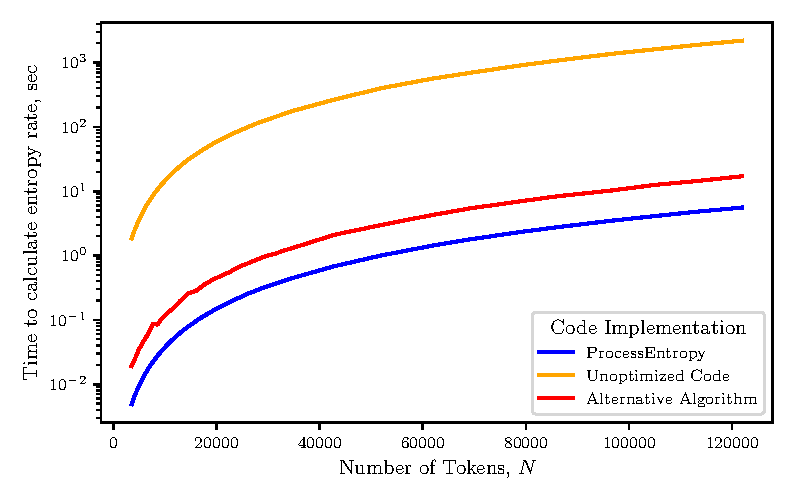
\includegraphics{chapter2/figs/speedcomparison.pdf}
\caption{A speed comparison of implementations of the Kontoyiannis entropy rate estimator. ProcessEntropy uses code from the package of the same name, unoptimized code is the same algorithm as ProcessEntropy without type and compile optimizations and Alternative Algorithm is an optimized alternative algorithm using the built-in \texttt{.contains()} method from the \texttt{stringlib} library. \label{fig:entropy:speedcomparison}}
\end{figure}


\autoref{fig:entropy:speedcomparison} shows a comparison of the optimized methods compared to alternatives. The ProcessEntropy package consistently performs the fastest, using the speed improvements listed above and efficient implementation. In contrast, the unoptimized code (written in pure Python without fixed type compiling or parallelisation) performs over two orders of magnitude slower for all input sizes. For comparison, an alternative algorithm is shown using the highly optimized \texttt{.contains()} method included in the \texttt{stringlib} library from Cython. This method uses a simplified version of the Boyer-Moore string-search algorithm, incorporating ideas from Horspool and Sunday~\cite{lundh_stringlib_2006}. Even with the alternative algorithm written in C, the ProcessEntropy code outperforms consistently. The package is available on the Python Package Index (PyPi) for interested researchers\footnote{\url{https://pypi.org/project/ProcessEntropy/}}.

\subsection{Running estimations}\label{sec:running_estimations}

To close this chapter, the tools developed throughout can now be applied to the news dataset introduced in \autoref{ch:data}. This news data contains 154 year-long Twitter content streams, with mean of 337,284 tokens. %
%(min 8059, max 2,627,305, $\sigma=$377,994)
Each stream has its entropy rate calculated and each pair of news-media outlets have their time-synced cross entropy rate calculated in both directions. In total this is 23,716 entropy rate estimations on these long sources. Even, with the efficient ProcessEntropy package, these calculations take well over a week, and this analysis would not be computationally tractable on the available hardware using the other implementations of the code.


\begin{figure}[!htbp]
	\centering
	\begin{subfigure}[t]{0.58\textwidth}
		\centering
		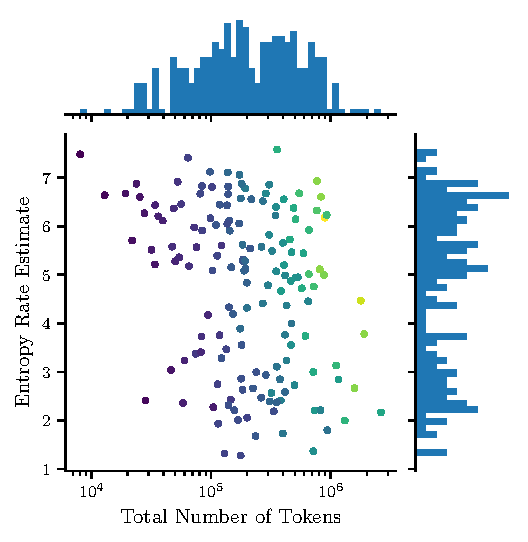
\includegraphics{chapter2/figs/tokens_vs_self_entropy_rate.pdf}
		\caption{}
	\end{subfigure}
	~
	\begin{subfigure}[t]{0.38\textwidth}
		\centering
		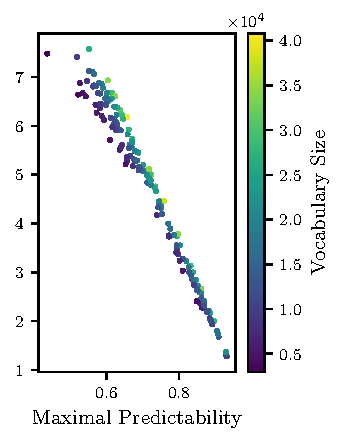
\includegraphics{chapter2/figs/entropy_vs_predictability.pdf}
		\caption{}
	\end{subfigure}
	\caption{Entropy rate estimates for the Twitter timelines of 154 news-media organisations during the calendar year of 2019. (a) shows the limited relationship between the total number of tokens in the Twitter text history and the entropy rate estimates. (b) shows the tight relationship between the entropy rates estimate and its derived maximal predictability, with higher variances seen at high entropies.}
	\label{fig:entropy:selfentropyrateestimates}
\end{figure}

\autoref{fig:entropy:selfentropyrateestimates} shows these entropy rate estimates on the news-media Twitter histories. Importantly, the entropy rate estimate shows very limited correlation with the total length of the content (number of tokens) or with the vocabulary size. This indicates that the estimate entropy rates have converged. Further, we see an expected strong correlation between the entropy rate estimate and the maximal predictability. Notably, the variance between the two increases for higher entropy rates, where larger vocabulary sizes can have an outsized effects on estimates. 

\begin{figure}[!htbp]
\centering
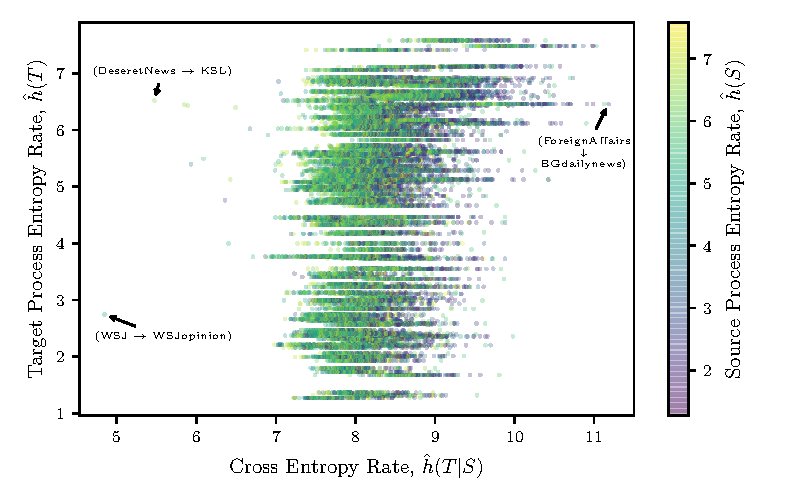
\includegraphics{chapter2/figs/cross_vs_self_entropy_rates.pdf}
\caption{Time-synced cross entropy rate estimates on pairs of news-media organisations on Twitter using their full content for the 2019 calendar year. Cross entropy rates are compared to the entropy rate estimates of the sources, $S$, and targets, $T$, in isolation. Example outliers are shown as `(source $\to$ target)'.} \label{fig:entropy:crossentropyestimates}
\end{figure}

Following this, the time-synced cross entropy rates are estimated and shown in \autoref{fig:entropy:crossentropyestimates}. Here we see similar results. The target entropy rate has limited correlation with the cross entropy rate ($R^2=0.116$), except for very high entropy targets, which receive higher cross entropy rates due to the high complexity nature of the target information. In contrast, source entropy rate has almost no correlation with the cross entropy rate ($R^2=0.0497$).

Several outliers exist at both the high and low ends of cross entropy. Low cross entropy outliers are all pairs of news-media organisations which are deeply related. Two examples of this are (\emph{@WSJ} $\to$ \emph{@WSJopinion}), where the information in the \emph{Wall Street Journal's} Opinion news stream can be described extremely efficiently by the \emph{Wall Street Journal's} main news stream, and (\emph{@DeseretNews} $\to$ \emph{@KSL}), where both news-media organisations report news specifically about Salt Lake City, Utah, and \emph{Deseret News} previously owned and remains closely linked to \emph{KSL}. 

At the high end of the cross entropy, pairs of organisations tend to have very little relationship. The highest cross entropy rate pair is (\emph{@ForeignAffairs} $\to$ \emph{@BGdailynews}) which suggests that very little information from the international relations focused \emph{Foreign Affairs Magazine} is useful in describing `Southcentral Kentucky's No. 1 Source for Information' \emph{Bowling Green Daily News}.

In total, the cross entropy rates are much higher than the entropy rates, highlighted in \autoref{fig:entropy:estimatedesnities}. This is an expected behaviour, as predicting the language and content behaviour of someone else is naturally harder than predicting your own future text. These distributional differences are carried over into maximal predictability, with generally lower maximal cross predictabilities.

\begin{figure}[!htbp]
	\centering
	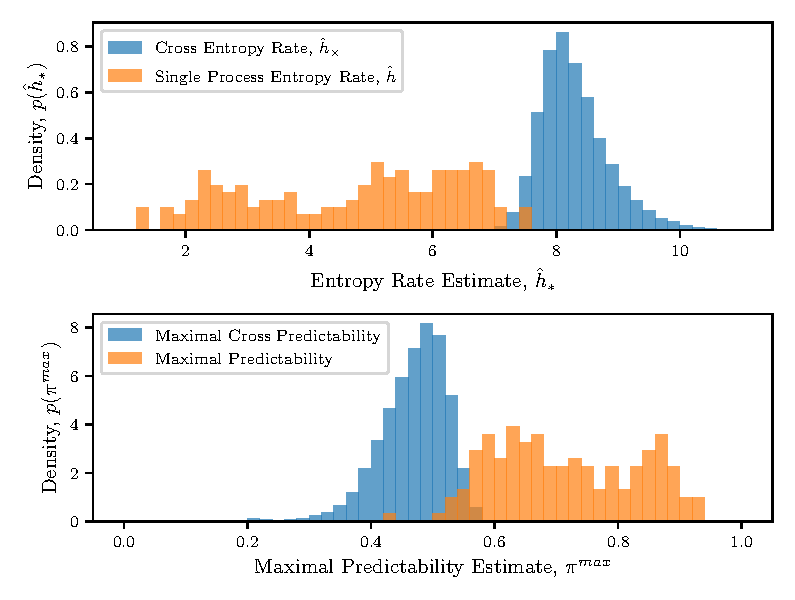
\includegraphics{chapter2/figs/entropy_densities.pdf}
	\caption{Comparison of cross and individual measures of information complexity. Self entropy rates and self maximal predictabilities are calculated for each of the 154 news-media organisations. Cross entropy rates and cross maximal predictabilities are calculated for all pairs of organisations. The distribution of the cross information and self information estimates are compared.
	Cross entropy rates are higher than self entropy rates as news-media organisations, in general, do not contain information in their history that is more useful to other news-media organisations than it is to themselves. This is reflected in the lower maximal cross predictabilities.  } \label{fig:entropy:estimatedesnities}
\end{figure}

\subsubsection{Concluding remarks}
Using both the Kontoyiannis entropy rate estimate and the generalised Kontoyiannis cross entropy rate estimate, we can construct a set of summary statistics about the language and behaviour patterns of the news sources under investigation and their relationships. These estimators are well founded on both a theoretical backbone and experimental evidence, and can be applied efficiently using the new open-source package, ProcessEntropy. From here, these calculated estimates can be used to extract the measures of information flow sought in this thesis, a task for \autoref{ch:quotermodel}.




%!TEX root = ../thesis.tex
\chapter{Creating robust information flow measures}\label{ch:quotermodel}

The question underpinning this work is how information flows between news organisations. The cross entropy rate estimation introduced in \autoref{ch:crossentropy} is an important tool to tackle this challenge, but is not sufficient in isolation. To understand information flow in the news-media ecosystem we need a tool that meets three criteria: (1) it must accurately identify how much information flows between outlets, (2) it must determine the direction of that flow, and (3) it must do so in the presence of information noise.

In this chapter we examine the efficiency of the cross entropy rate as a tool for measuring information flow, and introduce new measures derived from it. These measures are tested in a variety of simulated conditions using both synthetic and real language data to determine the best approach for quantifying information flow.


\section{The quoter model}
The `quoter model'~\cite{bagrow_quoter_2018} is a simple model for capturing the dynamics of information flow on networks. This model places $N$ individuals in a network connected by directed edges. These edges indicate that a quoting process is occurring from the source of the edge, $j$, to the target, $i$. This network of quoting across edges is designed to mimic the information generation process of users on social media, where users create content by either adding new information to the platform, or copying/quoting information already seen in their feed.

Each edge is assigned a quote probability, $q_{ji}$, and each node has a self generation probability, $q_{ii}$. These probabilities are used to decide how a node behaves at each time step of a simulation and are normalised such that $\sum_{\forall i} q_{ij} = 1$. The model repeatedly performs a process of text generation for $T$ steps. At each time point $t$, every node creates text through one of two processes.

With probability $q_{ii}$, the node \emph{self generates} a new sequence of words with length $\lambda(t) \sim L(t)$. $L(t)$ can be any length distribution that is representative of natural text lengths. These words are timestamped with $t$, and can be generated by drawing from any distribution of words or sequences. This new text is concatenated into a single timestamped sequence for each node at every time point, starting from $t=0$.

Alternatively, at each time point from $t=1$ onwards the node can undergo a \emph{quote process}. With probability $q_{ji}$, the target can quote from a source, $j$, by selecting a point in the source's sequence uniform randomly. The source's sequence includes only words generated before time $t$. Starting from the selected point in the source's history, a subsequence of length $\lambda(t) \sim L(t)$ is copied from the source's history into the present of the target, and is added to the target's timestamped sequence with time $t$.

Importantly, the quote process draws from the source's past indiscriminately, and could copy a sequence of text that the source had previous quoted from elsewhere. This sequence itself could originally generated by the target, and arrived in the source's history though a series of random quoting rounds. 

In general, this results in a system of information being passed between the nodes in the network, dependent of the quoting probabilities over the edges.

The \emph{self generation} process can use any arbitrary method for generating a sequence given a length $\lambda(t)$. In the case of the original model, two methods are used; drawing uniformly from a fixed vocabulary and drawing from a rank ordered vocabulary according to a Zipf distribution. In line with the previous chapter we use a Zipf distribution to generate text here.


\subsection{Single flow estimation} 

Previous work~\cite{bagrow_quoter_2018} used the Kontoyianni cross entropy rate to examine flow direction and quoting probability. This approach is reasonable, and deeply rooted in the quoter model construction. The quoter model produces sequences in the future of a quoter that exactly match the quoted source. It is these sequences which the match-length based cross entropy rate measure captures. However, this approach can break down when the producers of text have non-homogeneous text production methods.

We can see where this assumption of homogeneous generation is violated by performing an simple experiment. We take two text-producing nodes and connect them by a single edge, as in \autoref{fig:fixedalphasingleflow}(b). The node $S$ will always produce new text, without ever quoting. The node $T$ will follow the simple quoter model rules, producing new text of length $\lambda \sim Poi(3)$ with probability $1-q$ or quoting a length $\lambda$ from the history of the node $S$ with probability $q$. This link is simulated for a range of values for $q$ from 0 to 1. Both of these producers create their text by drawing from a Zipf distribution with scaling parameter~$\alpha=1.5$.

\begin{figure}[!htbp]
\centering
\includestandalone[width=\textwidth]{chapter3/figs/tikz/fixedalphasingleflow}
\caption{Simulations with node $S$ generating text from a Zipf distribution with scaling parameter $\alpha=1.5$ and node $T$ generating similarly with probability $1-q$ or quoting from $S$ with probability $q$. While the cross entropy rate is tightly correlated with $q$ (a), so two is the vocabulary size of $T$ (c) and the self entropy rate of $T$ (d). Simple linear models demonstrate that these comparison-free measures in (c) and (d) capture almost the same amount of explanatory information of $q$ as the cross entropy.}\label{fig:fixedalphasingleflow}
\end{figure}

We calculate the cross entropies between the two nodes in both directions, and other properties such as the entropy rate and vocabulary size of both $S$ and $T$ in isolation.

We perform separate linear regressions on the quoting probability for each of the properties, $h(T||S)$, $h(T)$ and the vocabulary. The properties and $q$ are transformed to a standard normal, with the logarithm of the vocabulary first being taken.
As expected, the cross entropy, $h(T||S)$ and $q$ have a significant negative linear relationship ($p<10^{-15}$), with 99.6\% of the variance explained. This result seems positive, but needs to be addressed in context. The cross entropy does show the relationship between the two sources, but is also influenced by the sequence properties of $T$.

A fitted linear model between the self entropy rate $h(T)$ and $q$ has a similar powerful negative linear relationship ($p<10^{-13}$, $R^2 = 0.886$). This result is a direct consequence of an important caveat of this model, its sensitivity to the vocabulary sizes of quote distributions. Indeed, the linear relationship between the normalised logged vocabulary of $T$ and the quote probability, $q$, shares the same predictive power ($p<10^{-13}$, $R^2 = 0.942$). This suggests that much of the predictive power in the cross entropy and self entropy rate is provided by the differences in vocabulary size between source and target. Hence, we first need to examine the the distributions of vocabulary size under quoting regimes before we can move on.

\subsubsection{Vocabulary sizes of quoted distributions}
% https://math.stackexchange.com/questions/32800/probability-distribution-of-coverage-of-a-set-after-x-independently-randomly/32816#32816
% https://math.stackexchange.com/questions/227556/the-exact-probability-of-observing-x-unique-elements-after-sampling-with-repla/1957820#1957820
This tight relationship between vocabulary size and quoting probabilities can be explained by sampling from a distribution with replacement. 
\begin{theorem}
Suppose we have a set of tokens $S$ with a fixed finite vocabulary size $V_S$. If we take a sample with replacement of size $N$ from $S$, this sample $T$ has a random vocabulary size $V_T$, according to the distribution,
$$P(V_T = v) = \frac{S_{2}(N, v) V_S!}{V_S^{N}(V_S-v)!},$$
where $S_2(\dot, \dot)$ is the Stirling number of the second kind~\cite{graham_concrete_1989}.
\end{theorem}
\begin{proof} %{of the vocabulary after sampling with replacement}
The vocabulary size is given by the number of unique elements in the sample. For a sample with vocabulary size $v$, each element must come from the set of size $V_S$. Hence, the number of possible vocabulary sets of size $V_T$ is $\binom{V_S}{v}$.


Given a sample vocabulary set (which has size $v$), we must choose how the elements that we draw are distributed amongst that vocabulary set. In essence, we have a set of $v$ bins that we can fill with our $N$ elements in our sample. Rephrased, we are finding the number of ways to partition $N$ elements into $v$ labelled sets, which is given by, $v! S_2(N, v).$


Together, this gives that the total number of possible samples with vocabulary size $v$ is,
$$ \binom{V_S}{v} v! S_2(N, v) =  \frac{ v! S_2(N, v) V_S! }{(V_S - v)! v!} = \frac{S_2(N, v) V_S! }{(V_S - v)!}.$$

Finally, we must divide by the total number of possible samples, $V_S^N$, which gives,
$$P(V_T = v) = \frac{S_{2}(N, v) V_S!}{V_S^{N}(V_S-v)!}.$$
\end{proof}


From this we find that the expected value for $V_T$ is,
$$E\left[V_T \right] = V_S\left(1-\left(1-\frac{1}{V_S}\right)^{N}\right) < V_S.$$ 

This highlights an important point, that when taking a finite sample with replacement, the expected vocabulary size of the sample will be \emph{lower} than the source.

This is a useful upper bound on the expectation of our quoter vocabularies. We expect the quoter model vocabularies sizes to be smaller again, due to the finite size of the text data during quoting. At early stages of the simulations, very little text exists in the source, and hence $V_S$ will be very small to start with. This means that under very high quote probabilities, $V_S$ must grow before $V_T$ can grow. 

We can see this result in \autoref{fig:vocabsizes}. Two nodes are again simulated with a single flow edge between then as per \autoref{fig:fixedalphasingleflow}. When there is no quoting between the nodes ($q=0$), meaning they both draw words identically and independently using the self generation process, the nodes have almost identical vocabulary distributions. The nodes are simulated 10,000 times for 1000 time steps of generation, giving a mean vocabulary size of 415 for both. However, when $q=1$ the target node is exclusively quoting from the source and does not produce text of its own. As expected from the above result, we see a significantly left-shifted vocabulary distribution, with the target node having a mean vocabulary size of 240. \autoref{fig:vocabsizes} reveals that this shift in vocabulary size change under increase $q$ is smooth, by running 10,000 simulations with $q \sim U(0,1)$.

\begin{figure}[!htbp]
\centering
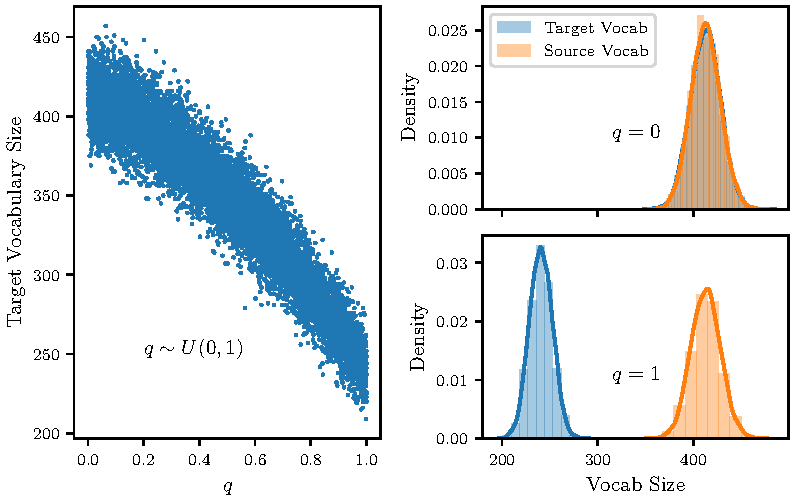
\includegraphics{chapter3/figs/VocabChangePlot.pdf}
\caption{A source produces text from a Zipf distribution of words. A target produces text similarly with probability $1-q$ or quotes from the source with probability $q$. The vocabulary size of the source and target are calculated by taking the number of unique elements after 1000 time steps. The vocabulary size of the target decreases as $q$ increases.}\label{fig:vocabsizes}
\end{figure}

\subsubsection{Variable vocabularies}
We next validate the ability of a measure to detect information flow beyond quoting. To achieve this, we introduce an extra dimension of variability to the model. 

We again have two text producers $S$ and $T$, shown in \autoref{fig:quoter_variable_vocab_tikz}, where $T$ quotes from $S$ with probability $q$. The source $S$ still creates text via a Zipf law distribution with scaling parameter $\alpha_S=1.5$, but the target $T$ now generates its own text at $\alpha_T \sim U(1.25,1.75)$. Having a larger scaling parameter will result in a smaller vocabulary distribution and \emph{vice versa}. This creates an interesting challenge for our measure. It needs to both account for the quoting along the edge, as well as natural variations in the text generation of $T$.

\begin{figure}[!htbp]
\centering
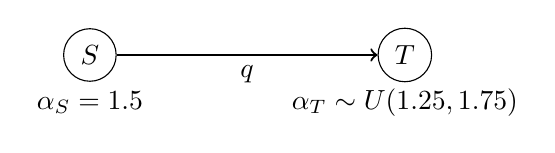
\begin{tikzpicture}[scale=2]
\node [draw, circle] (s) at (0, 0) {$S$};
\node [draw, circle] (t) at (2,0) {$T$}
edge [thick, <-] node[auto] {$q$} (s);

\node at (0,-0.3) {$\alpha_S = 1.5$};
\node at (2,-0.3) {$\alpha_T \sim U(1.25, 1.75)$};
\end{tikzpicture}
\caption{An diagram of a new quoting simulation regime. The target, $T$, now has a variable Zipf distribution scaling parameter for self generation, adding variability to the vocabulary size of its own self generated text.}\label{fig:quoter_variable_vocab_tikz}
\end{figure}

The single flow experiment is run with these new generation protocols to vastly different results. \autoref{fig:flow_variablealphascatterplot}, the simulations with very low quoting probabilities exhibit high variance in the vocabulary size, which is directly attributable to the choice of $\alpha_T$. As the quoting probability approaches 1, the amount of self generation of text by $T$ reduces resulting in a vocabulary of slightly under 66\% of the $S$ vocabulary size, as expected.


\begin{figure}[!htbp]
\centering
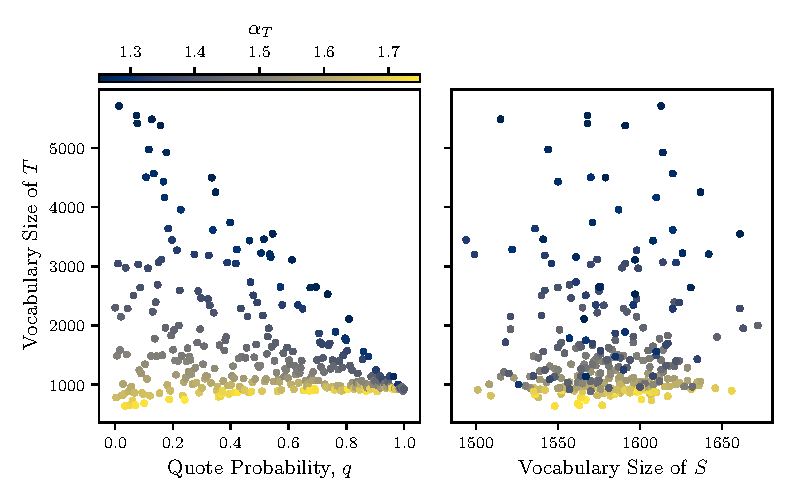
\includegraphics{chapter3/figs/VariableAlphaVocabSize.pdf}
\caption{The target node $T$ self generates with probability $1-q$ from a Zipf distribution according to a variable scaling parameter, $\alpha_T \sim U(1.25, 1.75)$. With probability $q$, $T$ quotes from the source, $S$, which always self generates with $\alpha_S = 1.5$. The added variability in the self generation $T$ decouples the tight previously correlation between the vocabulary size and the self generation probability. }\label{fig:flow_variablealphascatterplot}
\end{figure}

Again a linear model is fitted on $q$ using $h(T||S)$, with both variables being normalised. There is still a significant negative relationship ($p< 4\times10^{-6}$), but now with much less variance explained ($R^2 = 0.356$) compared the the previous experiment ($R^2=0.996$). In a similar fashion, both the self entropy rate and logged vocabulary size of $T$ have far lower explanatory power ($R^2=0.088$ and $R^2=0.163$ respectively).

Outside of simplified model conditions where text producers are identical, cross entropy rates are not themselves sufficient to identify the level of information flow. This is important as the real data discussed in \autoref{ch:data} has already been shown to have a wide range of vocabulary sizes. If only cross entropy rates were used on this data, the results would largely capture commonalities in vocabulary between pairs of organisations, and information flow measures would not be comparable. 

Performing a multiple linear regression on $q$ using a combination of variables provides a picture of how these variables relate. \autoref{tab:quoter_mutlipleOLS} shows models which combine $h(T||S)$ with the opposite direction cross entropy, $h(S||T)$, the self entropy rate of $T$, $h(T)$, and the self entropy rate of $S$, $h(S)$; with all variables being normalised. These models regressed on $q$ show a significant relationship with greater predictive power, hinting that more complex relationships between the metrics may be required to measures information across these edges. Indeed, in an environment where sources and targets have varying text generation parameters, such as in our real data, the use of other entropic estimates may be useful in controlling for these exogenous properties of the language. 

\begin{table}[!htbp]
\centering 
\begin{tabular}{c|cccc}
Variable& Model 1& Model 2& Model 3& Model 4\\ \hline
$h(S)$& & & & $-0.026^{**}$\\
$h(T||S)$& $-0.444^{***}$& $-0.814^{***}$& $-0.641^{***}$& $-0.742^{***}$\\
$h(T)$& & $0.679^{***}$& & $0.485^{***}$\\
$h(S||T)$& $0.343^{***}$& & & $0.132^{***}$\\
Vocab($T$)& & & $0.490^{***}$& \\\hline
\rule{0pt}{3ex}$R^2$& 0.876& 0.966& 0.626& 0.979\\ \hline
\rule{0pt}{3ex}adj. $R^2$& 0.871& 0.965& 0.610& 0.977\\ \hline
\multicolumn{5}{c}{$p_{val}<0.1^*$, $p_{val}<0.01^{**}$, $p_{val}<0.001^{***}$} \\ \hline\end{tabular}
\caption{Four ordinary linear regressions are fit on $q$ using the entropy rates of $S$ \& $T$, the cross entropy rates between $S$ \& $T$ in both directions, and the vocabulary size of T, Vocab($T$). These variables are calculated from 1000 simulations of $T$ quoting $S$ with probability $q\sim U(0,1)$, or $T$ self generating using $\alpha_T\sim U(1.25, 1.75)$ with probability $1-q$. $S$ always self generates using $\alpha_S = 1.5$. These models suggest that a combination of variables can help predict $q$ when $T$ and $S$ have different generation distributions.} \label{tab:quoter_mutlipleOLS}
\end{table}


\section{Novel measures of information flow}

To better capture the true flow of information in a network, a more robust measure may be needed. Here we introduce several possible measures and test them in larger simulated networks.

Our first measure is the most naive. We simply take the difference between the cross entropy rates in both directions, 
\begin{equation}a_{\hat{h}}  = \hat{h}(T||S) - \hat{h}(S||T).\end{equation}
Remembering that the measure needs to identify both the direction and magnitude of the flow across the edge, $a_{\hat{h}} >0$ indicates a flow from $S$ to $T$, and the reverse from $T$ to $S$ if $a_{\hat{h}} <0$. Further, a good metric should be able to distinguish between edges with and without flow ($q=0$). This first measure can be seen as an `absolute' measure.

In contrast, the second and third measures, 
\begin{equation}
b_{\hat{h}} := \frac{\hat{h}(T||S)}{\hat{h}(T)} - \frac{\hat{h}(S||T)}{\hat{h}(S)},
\end{equation}
and
\begin{equation}
c_{\hat{h}} := \frac{\hat{h}(T||S)}{\hat{h}(S)} - \frac{\hat{h}(S||T)}{\hat{h}(T)},
\end{equation}
normalise the cross entropy rates by the self entropy rates of the target, in $b_{\hat{h}}$, and the source, in $c_{\hat{h}}$. In theory, these self entropy rates may help create a fair comparison between the cross entropy rates in each direction.

For example, if a source was to have an extremely large vocabulary, or otherwise have complex language leading to a high information content, the cross entropy rate would be naturally inflated regardless of the quoting probability. Normalisation by entropy rate may hence improve detection.

The final set of measures seek to solve the problem of entropy normalisation, as well as the challenges of increased complexity of quote dynamics (such as the presence of quote cycles and chains of quoting) posed by larger networks. Measures, 
\begin{equation} d_{\hat{h}} := \frac{\hat{h}{(T||S)}}{\sum_X \hat{h}(X||T)} - \frac{\hat{h}(S||T)}{\sum_X \hat{h}(X||S)},\end{equation} 
and
\begin{equation} 
e_{\hat{h}} := \frac{\hat{h}(T||S)}{\sum_X \hat{h}(T||X)} - \frac{\hat{h}(S||T)}{\sum_X \hat{h}(T||X)},\end{equation}
seek to normalise the cross entropy rates using local neighbourhood network information, by dividing by the average cross entropy into the source ($d_{\hat{h}}$) or target ($e_{\hat{h}}$). 

This seeks to solve a deeper challenge, namely that in densely connected networks, there can be feedback loops and chains of information flow. Normalising using local network information may provide additional insight into the flow on single edges within the larger network.

So far we have discussed measures using only cross entropy rates and self entropy rates. For each metric we also consider the same measures with entropy rates $\hat{h}(T||S)$ replaced with predictabilities $\hat{\pi}(T||S)$. These predictabilities introduce a level of normalisation by the vocabulary of the target distribution. Greater flow likelihoods are represented by \emph{higher} predictabilities and \emph{lower} cross entropy rates; as such, the equations using $\hat{\pi}(T||S)$ are reversed in sign.

\autoref{tab:measures} shows the collection of all of the measures discussed here. 

\begin{table}[!htbp]
\centering
\begin{tabular}{cc}
 Entropy Based & Predictability Based  \\ 
\toprule
% \multirow{2}{*}{Naive}
 $ \displaystyle a_{\hat{h}} := \hat{h}(T||S) - \hat{h}(S||T)$ & 
$ \displaystyle a_{\hat{\pi}} := \hat{\pi}(S||T) - \hat{\pi}(T||S)$ \\
\midrule
% \multirow{2}{*}{Normalised}
 $ \displaystyle b_{\hat{h}} := \frac{\hat{h}(T||S)}{\hat{h}(T)} - \frac{\hat{h}(S||T)}{\hat{h}(S)}$ & 
$ \displaystyle b_{\hat{\pi}} := \frac{\hat{\pi}(S||T)}{\hat{\pi}(S)} - \frac{\hat{\pi}(T||S)}{\hat{\pi}(T)}$ \\
 $ \displaystyle c_{\hat{h}} := \frac{\hat{h}(T||S)}{\hat{h}(S)} - \frac{\hat{h}(S||T)}{\hat{h}(T)}$ & 
$ \displaystyle c_{\hat{\pi}} := \frac{\hat{\pi}(S||T)}{\hat{\pi}(T)} - \frac{\hat{\pi}(T||S)}{\hat{\pi}(S)}$ \\
\midrule 
% \multirow{2}{*}{Network}
 $ \displaystyle d_{\hat{h}} := \frac{\hat{h}(T||S)}{\sum_X \hat{h}(X||T)} - \frac{\hat{h}(S||T)}{\sum_X \hat{h}(X||S)}$ &
$ \displaystyle d_{\hat{\pi}} := \frac{\hat{\pi}(S||T)}{\sum_X \hat{\pi}(X||S)} - \frac{\hat{\pi}(T||S)}{\sum_X \hat{\pi}(X||T)}$  \\
\addlinespace[0.5ex]
 $ \displaystyle e_{\hat{h}} := \frac{\hat{h}(T||S)}{\sum_X \hat{h}(T||X)} - \frac{\hat{h}(S||T)}{\sum_X \hat{h}(T||X)}$ & 
$ \displaystyle e_{\hat{\pi}} := \frac{\hat{\pi}(S||T)}{\sum_X \hat{\pi}(T||X)} - \frac{\hat{\pi}(T||S)}{\sum_X \hat{\pi}(T||X)}$ \\
\end{tabular}
\caption{A glossary of the measures introduced to detect information flow.}\label{tab:measures}
\end{table}


\subsection{Network simulations}\label{sec:network_sizes}
To evaluate the quality of the information flow measures, we use quoter model simulations on larger networks to examine how the measures perform under various network types. 

In \autoref{fig:flow_networksize}, cliques are generated for sizes, $N=2$ to $N=50$. In the clique, each possible pair of nodes, $(j,i)$, is connected with a direction (bi-directional links are not allowed) and a preliminary edge quote probability, $q_{ji}' \sim U(0,1)$. Each node is assigned a self generation probability, $q_{ii}=0.5$. The incoming quote probabilities are normalised across the local incoming edges, 
$$q_{ji} = q_{ji}' / \left( \sum_{k\neq i} q_{ki}' + q_{ii} \right),$$
while the self generation probability is held constant. 

As above, the network undergoes a procedure of text generation wherein a node $i$ generates a new sequence of length $\lambda \sim Poi(3)$ from a Zipf distribution with scaling parameter $\alpha = 1.5$ or quotes a $\lambda$ long subsequence from neighbour $j$ with probability $q_{ji}$.

This generation procedure is performed for 7000 time steps to produce a quoter model network with sequences averaging $7000\times\mathbb{E}[\lambda]=21,000$ tokens. As we saw in \autoref{ch:crossentropy}, this is a sufficient number of tokens to allow for cross entropy convergence while balancing speed of computation. Cross entropy rates are calculated between every pair of edges and self entropy rates are calculated for every node. We then compute the information flow measures in \autoref{tab:measures}. For each network size, $M$, simulations were repeated such that there were at least 500 edges being estimated (e.g. $M=2$ requires 500 simulations while $M=3$ requires 167), with a minimum number of 4 simulations (e.g. $M=49$ has 1176 edges to estimate, but is repeated 4 times for a total of 4704 data points). For each $M$, the Pearson correlation coefficient is calculated between the true quote probability and the estimated information flow using each measure.

\begin{figure}[!htbp]
	\centering
	\begin{subfigure}[t]{\textwidth}
		\centering
		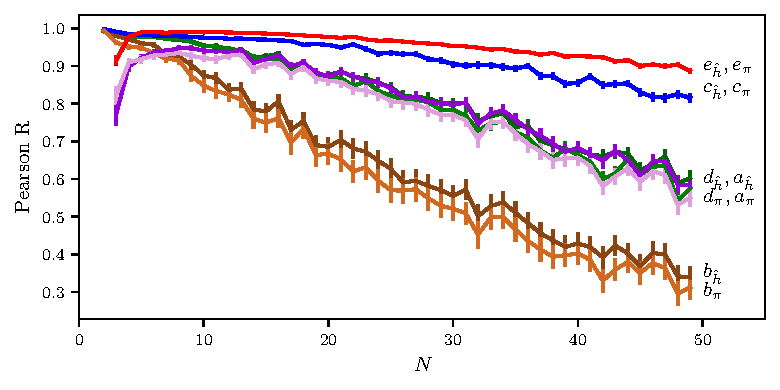
\includegraphics{chapter3/figs/zipf_network_size.pdf}
		\caption{Changing network size of random-orientation directed cliques}
		\label{fig:flow_networksize}
	\end{subfigure}

	\begin{subfigure}[t]{\textwidth}
		\centering
		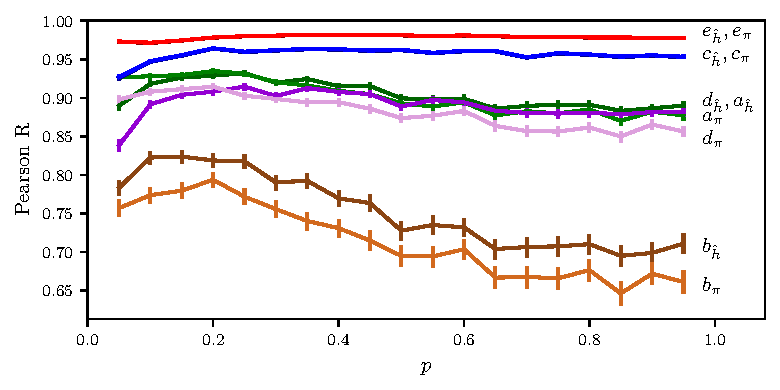
\includegraphics{chapter3/figs/zipf_ER.pdf}
		\caption{Changing edge probability of Erdős–Rényi networks. Density increases.}
		\label{fig:flow_ERchange}
	\end{subfigure}
	\caption{Networks are generated with a simulated quoter model and 95\% confidence intervals are shown for the Pearson correlation between the true quote probability and the estimated information flow for each flow measure. (a) shows simulations on directed networks with every pair of nodes having a directed single edge between them. Network size $N$ is varied, with larger networks resulting in smaller correlations. (b) takes an Erdős–Rényi network with 20 nodes and varying edge probability $p$. Flow correlations are consistent across $p$ for measures $e$ and $c$ despite increasing edge density while $b$ measures see a slight decline in performance. \label{fig:flow_sizeandER}}
\end{figure}

% Results
\autoref{fig:flow_networksize} shows that estimating quote probabilities becomes harder for larger network sizes. %
% This is expected as larger clique networks will have more self loops of quoting, and greater interdependence of text. 
Measures $e$ and $c$, which both normalise by the complexity of the target, outperform all others, with the local neighbourhood network information adding a slight improvement for $e$. These measure perform well using both cross entropy and cross predictability, with almost identical results which obscure the overlapping lines in the figure. Measures $a$ and $d$ perform equally well, with the predictability measures performing worse than the cross entropy measures. The tight relationship is surprising given that $a$ has no normalisation and $d$ normalises by the cross entropy / cross predictability into each source. Normalising by the source information proves counter productive, with $b$ have the lowest correlations between the true edge flows and estimated flows.

These trends are consistent as $N$ increases, with one caveat. For small $N$ ($\leq 5$) the local neighbourhood information based measures perform \emph{worse} than their non-network counterparts. % WHY?

A similar set of simulations is performed using a fixed size network ($N=20$) and directed edges generated randomly with probability $p$. Each edge in this Erdős–Rényi graph is assigned a quote probability and normalised exactly as above. All nodes self generate with a fixed probability $q_{ii}=0.5$. The general ranking of the measures remains consistent for all $p$ in \autoref{fig:flow_ERchange}. Measure $e$ consistently outperforms all other measures followed closely by measure $c$, this is likely as both measures $e$ and $c$ are normalising by the target complexity in both directions, with the network information giving a slight advantage to $e$. The rankings of measures $a$ and $d$ have similar Pearson correlation coefficients and remain close throughout. 

It is useful to remember that the Erdős–Rényi graph with $p=1$ is identical to the graph generation at point $N=20$ above. This approach will help us with the next question, disentangling the effect of edge quote probability and network complexity.   

\subsection{Disentangling complexity from quote probabilities}\label{sec:low_quote_probs}
% disentangling complexity vs low quote probabilities
With increasing network sizes comes both increasing conversational complexity and lower individual quote probabilities. This conversational complexity simply comes from having more nodes quoting each other. Whenever a quoting cycle appears (A quotes B; B quotes C; C quotes T) we could expect for difficulty in measuring the flow across individual edges, as the signal between the three would become mixed. As network size increases in a clique graph, more of these cycles appear.  

In addition to this, the increasing network size lowers the quote probabilities across each individual edge. As a directed clique graph with a single edge between each pair of node, each node will have an average of $(N-1)/2$ neighbours to quote from. Since the self generation probability is fixed at $q_{ii}=0.5$, the remaining neighbours must share the leftover probability between them. This results in lower quote probabilities across the edges, which provide less signal making them harder to detect amongst the noise.

\autoref{fig:flow_quote_scatterplot} shows these quote probability differences by comparing measures $a_{\hat{h}}$ and $e_{\hat{h}}$ against the edge quote probabilities ($q_{ij}$) from networks of size $N=8$ and $N=30$. The quote probability has a much larger range of [0,0.5] for the smaller $N=8$, with a smaller range [0, 0.14] for $N=30$.

The variance in the measures for low quote probabilities is very similar at both network sizes, however, the high quote probabilities of the small network add leverage to the Pearson correlation. In essence, we can view the underlying variance in flow estimates as a property of the language complexity. Sub-sequences of text can repeat themselves independently in different generators when both draw from the same or similar distributions. This noise is a property of the self generation process, not the quoting process. Given the fixed self generation probability, this aspect of variance is constant regardless of the quote probabilities. Indeed, when a no-intercept linear regression is performed for each $N$, the residuals exhibit homoscedasticity across the range of true quote probabilities and the standard deviation of the residuals is similar across all $N$ (95\% CI of $\sigma_{residuals}$: [0.186, 0.228]). 

Having high individual edge quote probabilities allows for the signal of those flows to be picked up through the noise, and leads to a stronger tail of high flow and high quote probability points. This naturally increases the Pearson correlation coefficient.

A common solution to high leverage points is to use a Spearman correlation coefficient, which uses ranks rather than values. However in this problem the Spearman correlation provides almost identical values to the Pearson. The higher value points are not outliers, but rather the tail end of a well-spread distribution across the [0,0.5] range, and low rank words still experience the same signal-noise trade-off as when comparing Pearson correlations for different distributions of edge quote probabilities.


\begin{figure}[!htbp]
	\centering
	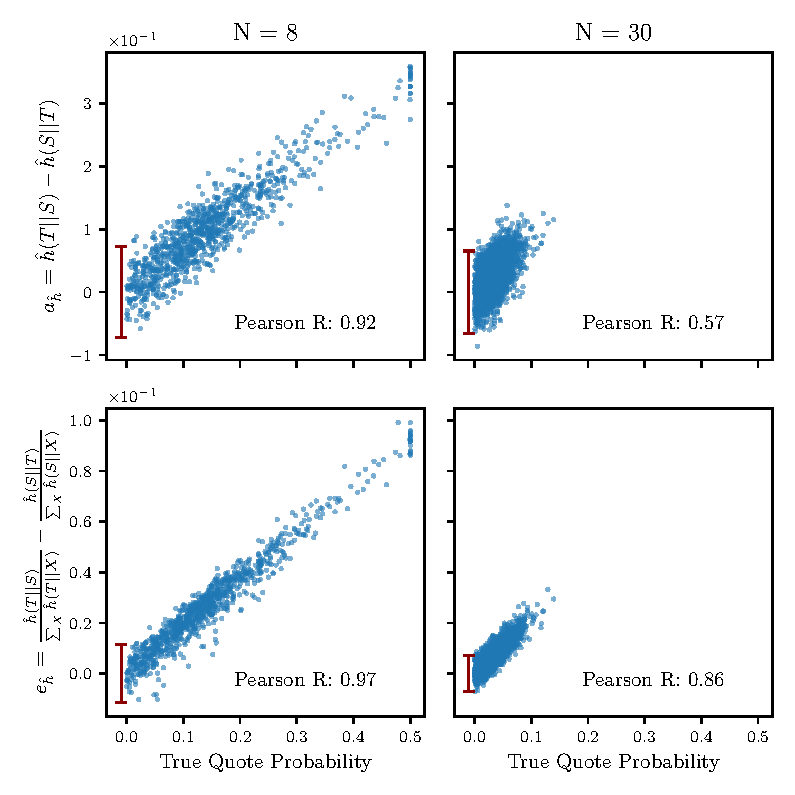
\includegraphics{chapter3/figs/scatterplot_comparison.pdf}
	\caption{Examples relationships between the true quote probability on a link between two notes and an information flow metric. Simple difference metrics such as $a_{\hat{h}}$ perform well on smaller networks with few nodes (N=3), but larger networks (N=30) need local neighbourhood information to perform well. For small networks, the tail high end quote probabilities pull up the Pearson correlation as they have stronger signal to overcome the constant variance from natural language generation. The {\color{red!40!black}dark red} bar shows the width of the 99\% confidence interval for the residuals of a no-intercept linear regression.}
	\label{fig:flow_quote_scatterplot}
\end{figure}

To further verify this effect we can vary the previous fixed self generation probability. As before, the edge quote probabilities normalise such that all generation and quote probabilities sum to one. Increasing $q_{ii}$ thus has the effect of shrinking these edge quote probabilities $q_{ji}$. If the above logic holds, then we would expect the increasing $q_{ii}$ values to decrease the Pearson correlation between $q_{ji}$ and the estimated flow. Indeed, in \autoref{fig:flow_self_p_vs_pearson_R} this pattern is observed with a clear decline in performance for all measures as the self generation probability increases. 


\begin{figure}[!htbp]
	\centering
	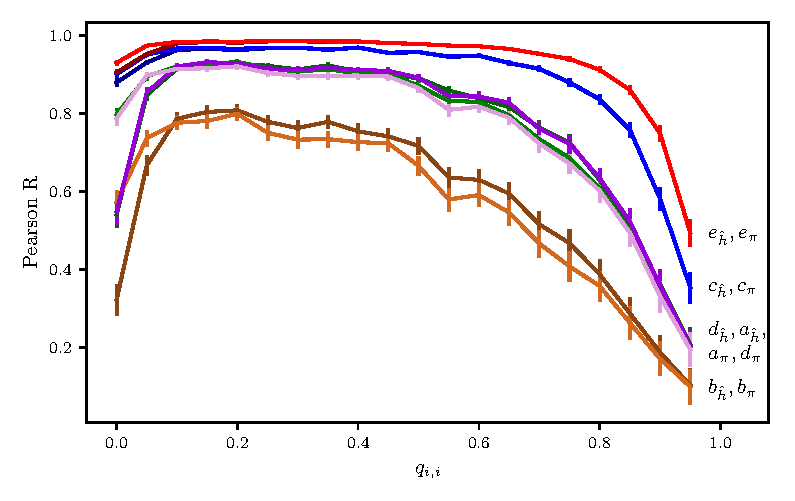
\includegraphics{chapter3/figs/zipf_self_p.pdf}
	\caption{Networks with 20 nodes are generated with each edge being assigned a direction and an edge quote probability $q_{ji}'$. The edge quote probabilities are added to the fixed self generation probability $q_{ii}$ and normalised. Increasing $q_{ii}$ decreases the edge quote probabilities on average which in turn decreases the Pearson correlation between the edge quote probabilities and the measured information flow. When no self generation is present ($q_{ii}=0$) only the generation seeds from $t=0$ are propagated, reducing measure performance.}
	\label{fig:flow_self_p_vs_pearson_R}
\end{figure}

Notably, there is also a decline in correlation at $q_{ii}=0$. In such a scenario the model would have all nodes quoting from one another based solely on the initial self generation step that seeds the process. This is surprising that even in an environment where limited source material exists, the measures still perform reasonably robustly.

\subsection{The effect of rewiring on measure performance}
In \autoref{sec:network_sizes}, we observed that increasing network size reduced the performance of information flow measures. \autoref{sec:low_quote_probs} showed that this is, in part, due to decreasing individual edge quote probabilities. However, increasing network size also increases the number of edges into and out-off each node. This leads to more cycles within the graph (even if they are of lower weights), making it difficult to determine sources of information. 

To isolate the effect of the network complexity on measure performance, we introduce a new simulated network. The Watts–Strogatz random graph model~\cite{watts_collective_1998} is used with a rewriting parameter $\beta$. In the model a graph is generated as a lattice, where each node in a network of size 20 is connected to its 8 nearest neighbours (without rewiring this is similar to an ER(20, 0.4) graph). These edges are assigned a random direction and weight, similar to the network models above. With probability $\beta$, the endpoint of each edge will rewire to attach to a random node. As $\beta$ increases, the network becomes less structured and more chaotic, with the clustering coefficient decreasing from its initial value of 0.64. In \autoref{fig:flow_zipf_watts_strogatz_model} these networks are generated for values of $\beta$ and the correlation coefficients are calculated for each measure. No trend is observed between $\beta$ and the correlation, indicating that the structural complexity of the network has no effect on measure performance when the distribution of individual quote probabilities are fixed. 

\begin{figure}[!htbp]
	\centering
	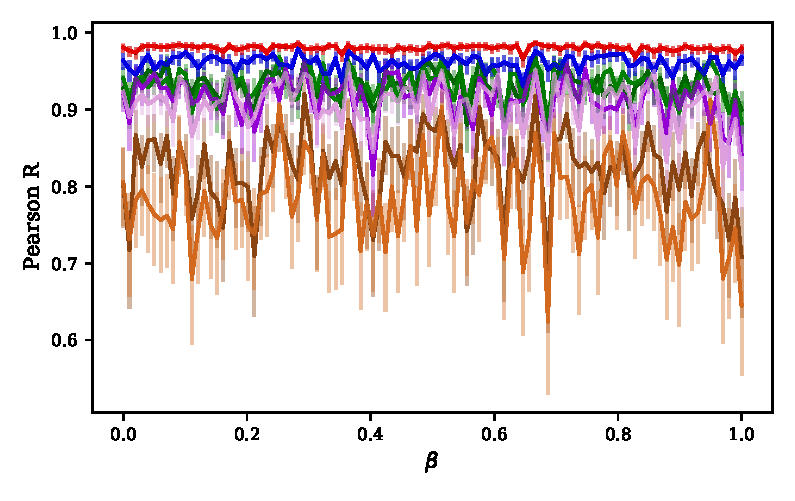
\includegraphics{chapter3/figs/zipf_watts_strogatz.pdf}
	\caption{A Watts–Strogatz random graph is generated with $N=20$ nodes and each edge assigned a direction and quote probability. These edges rewire with probability $\beta$. Information flow measures perform at consistent levels for all values of $\beta$, indicating that changing network structure has no impact on measure performance. 
	High variance in correlation is seen for measure {\color{brown}$b$ (brown)} with medium variance in {\color{violet}$d$ (purple)} and {\color{green!80!black}$a$ (green)}. This variance is exemplified by the large confidence intervals on the Pearson correlation coefficient which stands in contrast to the tight confidence intervals and low variance of measures {\color{red}$e$ (red)} and {\color{blue!80!black}$c$ (blue)}.}
	\label{fig:flow_zipf_watts_strogatz_model}
\end{figure}

This leads to the conclusion: the ability of the measures to correctly identify information flow is mostly dependent on the strength of the underlying quote probabilities to overcome the inherent noise present in text. While this conclusion is clear from the above results, they have used a simulated language model using Zipf distributions rather than real natural language. In order to confirm these results real data must be incorporated.


\section{Incorporating properties of real data}
A key limitation of the quoter model is the lack of foundation in real text data. Word generation processes such as those based on Zipf law are indeed derived from the analysis real data, but fall short of generating text that appears natural in most senses. The words generated using this method are independent, and lack the coherent structure of English grammar.

To rectify this, we update the \emph{self generation} process to use real text data. Using the corpus of Twitter data for news sources, each node in a simulated quoter graph is assigned a single news source. At each time step of the simulation a node can self generate by drawing a single random tweet from the entire history of the chosen outlets tweets and appending it to the node's timestamped sequence. The quoting process is identical, with each quote now drawing on sequences made from real tweets. Each simulation is run for 8000 time steps to maintain a consistent average sequence length. 

Since the average number of tweets for each news outlets is 19,337, drawing uniformly randomly with replacement would result in 33.9\% of tweets being drawn multiple times. To quickly prove this, assume we can draw a single tweet from $m$ tweets with probability $\frac{1}{m}$. The distribution of the number of times we draw that tweet over $N$ draws is $Binomial(N, \frac{1}{m})$, giving the cumulative probability that we draw it greater than one time being $1-\binom{N}{1} \frac{1}{m}(1-\frac{1}{m})^{N-1} - \binom{N}{0} (1-\frac{1}{m})^N = 1- Np(1-\frac{1}{m})^{N-1} - (1-\frac{1}{m})^N$. With $m=19337$ and $N=8000$ this gives 0.338783. To rectify this, tweets are drawn without replacement. 

\begin{figure}[!htbp]
	\centering
	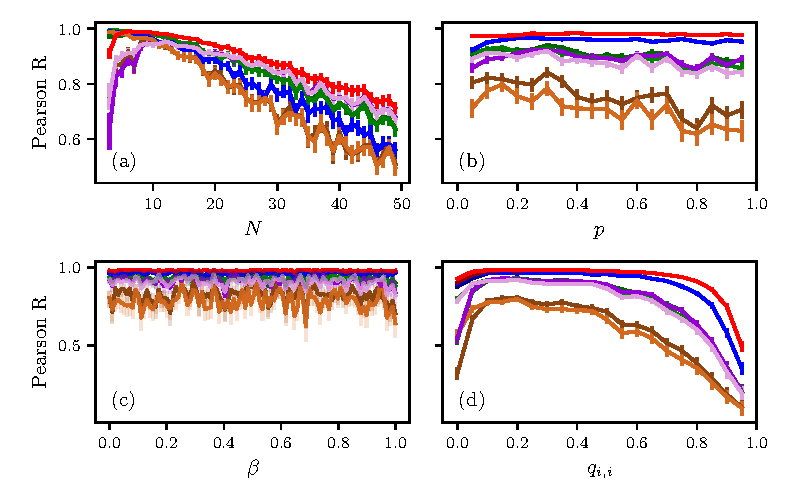
\includegraphics{./chapter3/figs/real_data_simulations.pdf}
	\caption{Networks are generated with $N$ nodes where each pair of nodes has an directed edge that exists with probability $p$ and is assigned a quote probability $q_{ji}'$. These quote probabilities are normalised such that their sum added to the fixed self generation probability, $q_{ii}$ equals 1. This self generation process draws from the Twitter history of a news outlet which is assign at network creation. (b), (c) and (d) use $N=20$ while (a) varies $N$. (a), (b) and (c) use $q_{ii}=0.5$ while (d) varies $q_{ii}$.  (a) and (d) use $p=1$ while (b) varies $p$ and (c) uses a more sophisticated Watt-Strogatz model which starts as a lattice with $p=0.4$ and requires edge endpoints with probability $\beta$. All simulations using real data for text generation follow the same results as their counterpart experiments using Zipf distributions for text generation.}
	\label{fig:flow_realdataquotermodel}
\end{figure}

Using this new self generation process the same experiments are run as above. \autoref{fig:flow_realdataquotermodel} combines the results from \autoref{fig:flow_sizeandER}, \autoref{fig:flow_self_p_vs_pearson_R} and \autoref{fig:flow_zipf_watts_strogatz_model}, updated to use real data. The core results outlined above remain exactly the same when using real data in place of simulated text in the model. 


\section{Go with the flow: applying the information flow measure}\label{sec:gowiththeflow}
\subsubsection{Selecting the best measure}
Put together, the results in this chapter suggest two key findings; the cross entropy is not a sufficient measure of information flow without normalising by the target entropy properties; and the information contained in the local neighbourhood structure is more informative than the entropy rate of a target alone.

Throughout every comparison done here the ranking of the measures fall into four categories.
\begin{itemize}
\item Measures $e_{\hat{h}}$ and $e_{\hat{\pi}}$ consistently outperform all other measures for networks of size greater than 5. These measures work by normalising the cross entropy or cross predictability using the local neighbourhood cross entropies or cross predictabilities going into the \emph{target}. While both types of the measure perform equally well in the large networks, the measure under-performs for networks with less than 5 nodes, as expected given the limited neighbourhood information.

\item Measures $c_{\hat{h}}$ and $c_{\hat{\pi}}$ perform slightly worse than the $e$ measures in large networks, but still hold their own. These measures work by normalising by the entropy or predictability of the \emph{target} without any knowledge of the network structure. Indeed, the lack of required network information allows this measure to perform the best for very small networks.

\item Measures $a_{\hat{h}}$,  $a_{\hat{\pi}}$, $d_{\hat{h}}$ and $d_{\hat{\pi}}$ perform consistently poorly when quote probabilities become low. The similarly between these measures is somewhat surprising given that $a$ has no normalisation while $d$ normalises by the local neighbourhood of the \emph{source}; indicating that the source neighbourhood provides almost no value to the calculation of flow.

\item Indeed, measures $b_{\hat{h}}$ and $b_{\hat{\pi}}$ which normalise by the entropy rate or predictability of the source without network information perform even worse than the simple difference between un-normalised cross entropies. 
\end{itemize}

From these results we find that $e_{\hat{h}}$ and $e_{\hat{\pi}}$ are clear the best measures. While either measure would be suitable in synthetic conditions, we choose to use $e_{\hat{\pi}}$ as we apply the measure to real data. In the simulations throughout this chapter we have seen the impact of vocabulary size on the measurement of information flow. As the real variety of text produces variety in vocabulary by an order of magnitude, we use the predictability version to help further counteract the impact of the vocabulary. 

Hence, we move forward using the measure,
\begin{equation} 
e_{\hat{\pi}} := \frac{\hat{\pi}(S||T)}{\sum_X \hat{\pi}(T||X)} - \frac{\hat{\pi}(T||S)}{\sum_X \hat{\pi}(T||X)}
\end{equation}
as the most robust tool to estimate information flows in networks of natural language text. 

\subsubsection{Results of applying the best measure}

Using measure $e_{\hat{\pi}}$ we can perform estimates of information flow between each pair of news organisations. In \autoref{sec:running_estimations} we performed the estimation of the entropy rates and cross entropy rates between all pairs of organisations using the entire corpus of tweets by each organisation for the 2019 calender year. Once these estimates are calculated, applying the information flow measure is computationally simple final step to extracting the estimates of flow. \autoref{fig:flow_appliedtodata} shows the distribution of these estimates for all pairs of organisations. As $e_{\hat{\pi}}$ is symmetrical around 0 when you swap the source and target, we choose the positive flow as the direction of the edge and assign its weight to be the flow estimate.

% \begin{figure}[!htbp]
% 	\centering
% 	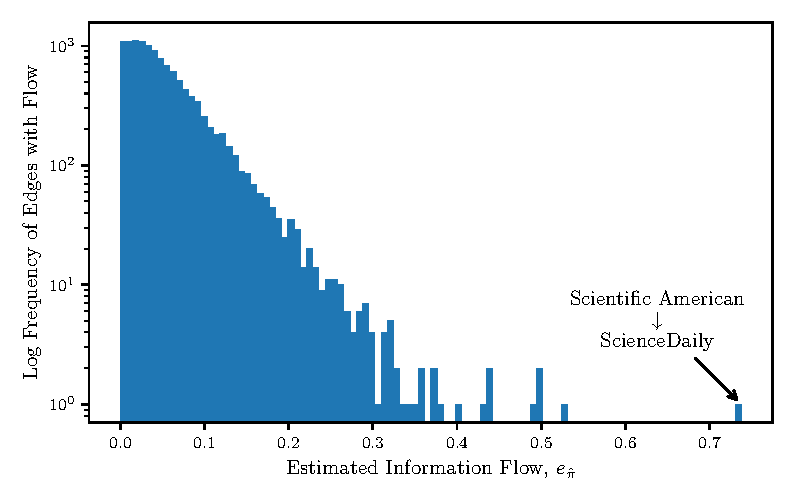
\includegraphics{./chapter3/figs/edge_weights.pdf}
% 	\caption{Information flow is estimated using measure $e_{\hat{\pi}}$ between each pair of news-media organisations using their entire tweet corpus. Each edge is assigned a direction and the positive weights of those edges are shown here. Most edges show very little information flows with only 1.6\% of edges having a flow estimate above 0.2. }
% 	\label{fig:flow_appliedtodata}
% \end{figure}

\begin{figure}[!htbp]
	\centering
	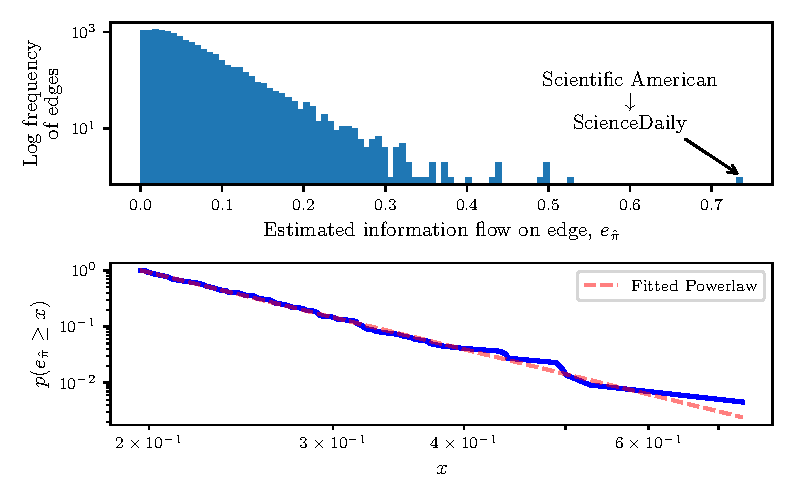
\includegraphics{./chapter3/figs/edge_weights_ccdf.pdf}
	\caption{\ts{This is your CCDF Matt. I'm not sure how much information this actually adds. Should we keep it?} Information flow is estimated using measure $e_{\hat{\pi}}$ between each pair of news-media organisations using their entire tweet corpus. Each edge is assigned a direction and the positive weights of those edges are shown. Most edges show very little information flows with only 1.6\% of edges having a flow estimate above 0.2. A complementary cumulative distribution function is shown with a fitted power law with exponent 5.6. }
	\label{fig:flow_appliedtodata}
\end{figure}

It is important to note that these flow estimates are not directly measuring a proportion of tweets that are copied, but rather a relative measure of how much informational content of the source is present in the target, compared to other pairs of organisations. 

Two key features of \autoref{fig:flow_appliedtodata} stand out: the heavy right skew of the distribution and the few outliers. Of the edges weight, 98.4\% are less that 0.2 leaving only 199 edges with weight greater than 0.2. This is important to note as \autoref{sec:low_quote_probs} highlighted that flow estimates are harder to disentangle from the noise of natural language when the information flow is low. Much of the flow estimate edges may be detecting a weak flow purely due to the commonality of their natural language. 

Noting the challenge created by information noise, these flow edges are useful for two purposes: comparing the magnitude of flows between two different pairs, and identifying the direction of flow when the flow estimate is large enough. As an example of the first, we can find that, as an information source, the \emph{New York Times} has relatively little net information flow to the \emph{Washington Post} (0.0053) but relatively high net information flow to the \emph{Foreign Affairs Magazine} (0.1480).

As an example of the second purpose, we examine the highest flow edge in the network, from the \emph{Scientific American} to \emph{ScienceDaily}.  This edge with weight (0.7378) is likely due to a confounding of factors. Firstly, \emph{Scientific American} is a popular and well resourced organisation that produces a large volume of content. The smaller and less popular \emph{ScienceDaily} is unlikely to get the `scoop' on many scientific stories meaning most content it posts will exist in the history of \emph{Scientific American}. Finally, \emph{ScienceDaily} has the least tweets, tokens and second least vocabulary of any organisation. This makes the normalisation of the information flows difficult due to its vocabulary being at the extreme of the distribution. 

In constructing these weighted edges into a network, it would be ideal to filter out low flow edges to make the graph more sparse for analysis. However, choosing such cut-offs can prove dubious at best. In the next chapter we explore several methods of using this network to rank the net information influence of news-media organisations and examine the inconsistency in their results.


% add as many as you like

\appendix
% Import the appendices 
% %!TEX root = ../thesis.tex
\chapter{News Media Twitter Accounts\label{app:accounts}}

\subsection{Included Organisations}

\begin{table}[h]
	\caption{\todo{Caption}}
	\label{appendix:tab:accounts_0}
	\begin{center}
		\resizebox{1 \textwidth}{!}{\begin{tabular}{lllrr}
\toprule
                    Name &  Twitter Account & Assigned Bias &  Number of Tweets &  Followers \\
\midrule
      The New York Times &          nytimes &     Lean Left &             31029 &   44800317 \\
                     CNN &              cnn &          Left &             57155 &   44153462 \\
        BBC News (World) &         BBCWorld &        Center &             11679 &   26446876 \\
           The Economist &     theeconomist &     Lean Left &             35771 &   24239639 \\
                 Reuters &          reuters &        Center &            128448 &   21042215 \\
 The Wall Street Journal &              WSJ &        Center &             32151 &   17139922 \\
                    TIME &             time &     Lean Left &             29631 &   16512854 \\
                  Forbes &           Forbes &        Center &             31940 &   15736852 \\
                ABC News &              ABC &     Lean Left &             44149 &   14804638 \\
     The Washington Post &   washingtonpost &     Lean Left &             45043 &   14644580 \\
    The Associated Press &               ap &        Center &             10214 &   13671750 \\
                HuffPost &         huffpost &          Left &             27622 &   11472382 \\
              TechCrunch &       techcrunch &        Center &             14348 &   10124437 \\
                Mashable &         mashable &          Left &             40854 &    9809420 \\
          The New Yorker &        newyorker &          Left &             13948 &    8774527 \\
          The Daily Show &     thedailyshow &     Lean Left &              3386 &    8256511 \\
            The Guardian &         guardian &     Lean Left &             77532 &    8243012 \\
                     NPR &              npr &        Center &             21236 &    7959364 \\
                CBS News &          CBSNews &     Lean Left &             34060 &    7078950 \\
           Rolling Stone &     RollingStone &          Left &             18571 &    6295950 \\
               Bloomberg &         business &        Center &            109367 &    5790419 \\
             VANITY FAIR &       vanityfair &     Lean Left &             15585 &    4887894 \\
                   TODAY &        TODAYshow &     Lean Left &             17678 &    4282063 \\
              Lifehacker &       lifehacker &        Center &              9026 &    4153410 \\
                POLITICO &         politico &     Lean Left &             25742 &    4016243 \\
               USA TODAY &         usatoday &        Center &             27303 &    3949159 \\
         Financial Times &               FT &        Center &             41030 &    3806483 \\
     Scientific American &            sciam &        Center &              2335 &    3805593 \\
                The Hill &          thehill &        Center &            157172 &    3501890 \\
       Los Angeles Times &          latimes &     Lean Left &             35341 &    3473994 \\
                Newsweek &         newsweek &     Lean Left &             46922 &    3407905 \\
              Teen Vogue &        TeenVogue &     Lean Left &             12270 &    3358001 \\
                    CNBC &             cnbc &        Center &             66578 &    3355408 \\
                   MSNBC &            msnbc &          Left &             32699 &    2870702 \\
        Business Insider &  businessinsider &        Center &             57915 &    2790009 \\
           The Telegraph &        Telegraph &    Lean Right &             24235 &    2774439 \\
               The Verge &            verge &     Lean Left &             19096 &    2613577 \\
       Daily Mail Online &       MailOnline &         Right &             28671 &    2437611 \\
                    VICE &             vice &          Left &             17195 &    2000034 \\
                   CSPAN &            cspan &        Center &              5022 &    1989017 \\
\bottomrule
\end{tabular}
}
	\end{center}
\end{table}

\begin{table}[h]
	\caption{\todo{Caption}}
	\label{appendix:tab:accounts_1}
\begin{center}
\resizebox{1 \textwidth}{!}{\begin{tabular}{lllrr}
\toprule
                   Name & Twitter Account & Assigned Bias &  Number of Tweets &  Followers \\
\midrule
           The Atlantic &     theatlantic &     Lean Left &             15100 &    1850164 \\
      New York Magazine &           NYMag &          Left &             19072 &    1800255 \\
                  Slate &           slate &          Left &             58598 &    1792093 \\
        Al Jazeera News &         AJENews &        Center &             11252 &    1573047 \\
          New York Post &          nypost &         Right &             79771 &    1543609 \\
          BuzzFeed News &    BuzzFeedNews &     Lean Left &             19705 &    1338555 \\
         Breitbart News &   BreitbartNews &         Right &             17501 &    1225203 \\
             Yahoo News &       YahooNews &          Left &             19781 &    1106092 \\
        Chicago Tribune &  chicagotribune &        Center &             22994 &    1099101 \\
                    AJC &             ajc &     Lean Left &             27978 &    1045546 \\
           PBS NewsHour &        NewsHour &        Center &             16189 &    1036993 \\
                  Salon &           salon &          Left &             11614 &     976078 \\
                    Vox &       voxdotcom &          Left &             17574 &     891290 \\
             ProPublica &      propublica &        Center &              6458 &     833038 \\
           Mother Jones &     motherjones &          Left &             16447 &     809121 \\
       The Boston Globe &     bostonglobe &     Lean Left &             49224 &     756522 \\
          The Intercept &    theintercept &          Left &              6642 &     753001 \\
    New York Daily News &     nydailynews &          Left &             28682 &     728512 \\
        Foreign Affairs &  ForeignAffairs &        Center &             11964 &     724994 \\
 New York Times Opinion &      nytopinion &          Left &             25402 &     718663 \\
         Democracy Now! &    democracynow &          Left &              9453 &     710714 \\
               TheBlaze &        theblaze &         Right &             13121 &     706991 \\
           Daily Caller &     DailyCaller &         Right &             34716 &     579741 \\
               The Root &         TheRoot &     Lean Left &              6994 &     525879 \\
               Upworthy &        upworthy &          Left &              1472 &     511090 \\
       One America News &            OANN &    Lean Right &              6108 &     510392 \\
      Chicago Sun-Times &        Suntimes &     Lean Left &             15976 &     505161 \\
                 SFGate &          sfgate &     Lean Left &             17838 &     477782 \\
           Miami Herald &     MiamiHerald &     Lean Left &             19290 &     450869 \\
     The Jerusalem Post &  Jerusalem\_Post &        Center &             29868 &     445004 \\
                Esquire &         esquire &          Left &             12817 &     418881 \\
                 Quartz &              qz &        Center &             28604 &     384220 \\
   The Washington Times &       WashTimes &    Lean Right &             34635 &     372421 \\
              Roll Call &        rollcall &        Center &             10157 &     361580 \\
         The Daily Wire &   realdailywire &         Right &             26385 &     361505 \\
        National Review &             NRO &         Right &             16572 &     336300 \\
                  Axios &           axios &        Center &             19184 &     315533 \\
       Austin Statesman &       statesman &     Lean Left &              9562 &     300429 \\
              Daily Kos &        dailykos &          Left &             12636 &     280636 \\
                 reason &          reason &    Lean Right &              7939 &     242262 \\
\bottomrule
\end{tabular}
}
\end{center}
\end{table}

\begin{table}[h]
	\caption{\todo{Caption}}
	\label{appendix:tab:accounts_2}
	\begin{center}
		\resizebox{1 \textwidth}{!}{\begin{tabular}{lllrr}
\toprule
                    Name &  Twitter Account & Assigned Bias &  Number of Tweets &  Followers \\
\midrule
            Mercury News &         mercnews &     Lean Left &             36535 &     241228 \\
                 Jacobin &       jacobinmag &          Left &              8579 &     241092 \\
            ScienceDaily &     sciencedaily &        Center &              1243 &     240013 \\
           Las Vegas Sun &      LasVegasSun &     Lean Left &              8233 &     238797 \\
                   grist &            grist &     Lean Left &              6438 &     230344 \\
      The Sacramento Bee &      sacbee\_news &     Lean Left &             22511 &     219066 \\
                RedState &         redstate &         Right &             19778 &     218545 \\
          The Federalist &           FDRLST &         Right &              5830 &     217053 \\
           O.C. Register &       ocregister &    Lean Right &             23872 &     212517 \\
               SF Weekly &         sfweekly &        Center &              4438 &     210524 \\
               Raw Story &         rawstory &          Left &             29702 &     205992 \\
     Washington Examiner &       dcexaminer &    Lean Right &             61833 &     198229 \\
                OBSERVER &         observer &        Center &              5856 &     195067 \\
 San Francisco Chronicle &      sfchronicle &          Left &             18021 &     189685 \\
                     KSL &           KSLcom &         Right &             11881 &     179424 \\
                Truthout &         truthout &     Lean Left &              7806 &     170572 \\
        The New Republic &      newrepublic &          Left &             10725 &     167916 \\
           Investors.com &     IBDinvestors &    Lean Right &              2469 &     167242 \\
 Pittsburgh Post-Gazette &     PittsburghPG &    Lean Right &             24711 &     166684 \\
       Commercial Appeal &      memphisnews &     Lean Left &             15885 &     162002 \\
                Mediaite &         Mediaite &     Lean Left &             14030 &     159980 \\
            Townhall.com &      townhallcom &         Right &             10452 &     152082 \\
               U.S. News &           usnews &     Lean Left &             12827 &     150674 \\
                AlterNet &         alternet &          Left &              7156 &     139194 \\
        National Journal &  nationaljournal &        Center &              1424 &     133097 \\
                The Week &          theweek &        Center &              9031 &     129703 \\
                CBN News &          CBNNews &         Right &             15627 &     128487 \\
    Intl. Business Times &          IBTimes &        Center &             11519 &     123358 \\
             CNSNews.com &          cnsnews &         Right &              9035 &     119236 \\
          Times-Dispatch &          RTDNEWS &    Lean Right &              7018 &     116510 \\
             Free Beacon &       FreeBeacon &         Right &              9091 &     110634 \\
           Boston Herald &     bostonherald &    Lean Right &             12550 &     105046 \\
                 Newsmax &          newsmax &         Right &              3825 &     100437 \\
         Current Affairs &       curaffairs &          Left &              2188 &      99136 \\
            Deseret News &      DeseretNews &    Lean Right &             15087 &      97060 \\
      WSJ Editorial Page &       WSJopinion &    Lean Right &              4990 &      96734 \\
                  Bustle &           bustle &     Lean Left &              1504 &      96170 \\
         Courier Journal &   courierjournal &     Lean Left &             13988 &      88551 \\
   Portland Press Herald &      PressHerald &        Center &              6372 &      85834 \\
             Defense One &       DefenseOne &        Center &              6892 &      81992 \\
\bottomrule
\end{tabular}
}
	\end{center}
\end{table}

\begin{table}[h]
	\caption{\todo{Caption}}
	\label{appendix:tab:accounts_3}
	\begin{center}
		\resizebox{1 \textwidth}{!}{\begin{tabular}{lllrr}
\toprule
                                     Name &  Twitter Account & Assigned Bias &  Number of Tweets &  Followers \\
\midrule
                               The Nation &       The\_Nation &          Left &             13048 &      78860 \\
            The Christian Science Monitor &        csmonitor &        Center &              5676 &      75406 \\
                      AR Democrat-Gazette &   ArkansasOnline &          Left &             10951 &      74177 \\
                                INDY Week &         indyweek &     Lean Left &              4175 &      73802 \\
                             PoliticusUSA &     PoliticusUSA &          Left &              7253 &      72856 \\
                         The Daily Signal &      Dailysignal &         Right &              6740 &      68024 \\
                                 PJ Media &      PJMedia\_com &    Lean Right &              5666 &      66324 \\
                              Delco Times &       delcotimes &     Lean Left &              3302 &      64714 \\
                              Daily Press &      Daily\_Press &    Lean Right &              3512 &      61225 \\
                            YES! Magazine &      yesmagazine &          Left &              4679 &      60455 \\
                          SpokesmanReview &  SpokesmanReview &     Lean Left &              4113 &      58352 \\
                     Tallahassee Democrat &         TDOnline &          Left &             15098 &      53700 \\
                         The Korea Herald &   TheKoreaHerald &        Center &              8730 &      53517 \\
                       The Michigan Daily &    michigandaily &     Lean Left &              2041 &      50748 \\
                      Honolulu Civil Beat &        CivilBeat &        Center &              1837 &      50503 \\
                     Libertarian Republic &   TheLibRepublic &    Lean Right &              1145 &      47475 \\
                The American Conservative &         amconmag &    Lean Right &             25197 &      46189 \\
                   The American Spectator &      amspectator &         Right &              1915 &      45877 \\
                          The Red \& Black &      redandblack &        Center &              7663 &      42735 \\
                                KQED News &         kqednews &        Center &              8655 &      41720 \\
                    Indiana Daily Student &          idsnews &        Center &              3867 &      41621 \\
                                     WGBH &             wgbh &        Center &              2211 &      39971 \\
                      The Western Journal &   WestJournalism &         Right &              7114 &      38478 \\
                      Commentary Magazine &       Commentary &         Right &              1337 &      35704 \\
                       The Daily Progress &    DailyProgress &        Center &              6856 &      35506 \\
                                 VTDigger &         vtdigger &     Lean Left &              5671 &      32820 \\
                            BG Daily News &      bgdailynews &     Lean Left &              7686 &      22341 \\
                      Longmont Times-Call &        TimesCall &     Lean Left &              3858 &      21077 \\
                   The Daily Northwestern &       thedailynu &     Lean Left &              4580 &      20357 \\
 Right Side News: Breaking News \& Opinion &    rightsidenews &         Right &              4033 &      17600 \\
                                     WFAE &             wfae &        Center &              4317 &      17385 \\
                          The College Fix &       CollegeFix &         Right &              4094 &      15289 \\
                            The Chronicle &    DukeChronicle &        Center &              1537 &      15207 \\
                               CalMatters &       calmatters &        Center &              3247 &      15069 \\
\bottomrule
\end{tabular}
}
	\end{center}
\end{table}


%
%
%\begin{center}
%	\captionof{table}{\todo{Caption}}
%	\resizebox{1 \textwidth}{!}{\begin{tabular}{lllrr}
\toprule
                    Name &  Twitter Account & Assigned Bias &  Number of Tweets &  Followers \\
\midrule
      The New York Times &          nytimes &     Lean Left &             31029 &   44800317 \\
                     CNN &              cnn &          Left &             57155 &   44153462 \\
        BBC News (World) &         BBCWorld &        Center &             11679 &   26446876 \\
           The Economist &     theeconomist &     Lean Left &             35771 &   24239639 \\
                 Reuters &          reuters &        Center &            128448 &   21042215 \\
 The Wall Street Journal &              WSJ &        Center &             32151 &   17139922 \\
                    TIME &             time &     Lean Left &             29631 &   16512854 \\
                  Forbes &           Forbes &        Center &             31940 &   15736852 \\
                ABC News &              ABC &     Lean Left &             44149 &   14804638 \\
     The Washington Post &   washingtonpost &     Lean Left &             45043 &   14644580 \\
    The Associated Press &               ap &        Center &             10214 &   13671750 \\
                HuffPost &         huffpost &          Left &             27622 &   11472382 \\
              TechCrunch &       techcrunch &        Center &             14348 &   10124437 \\
                Mashable &         mashable &          Left &             40854 &    9809420 \\
          The New Yorker &        newyorker &          Left &             13948 &    8774527 \\
          The Daily Show &     thedailyshow &     Lean Left &              3386 &    8256511 \\
            The Guardian &         guardian &     Lean Left &             77532 &    8243012 \\
                     NPR &              npr &        Center &             21236 &    7959364 \\
                CBS News &          CBSNews &     Lean Left &             34060 &    7078950 \\
           Rolling Stone &     RollingStone &          Left &             18571 &    6295950 \\
               Bloomberg &         business &        Center &            109367 &    5790419 \\
             VANITY FAIR &       vanityfair &     Lean Left &             15585 &    4887894 \\
                   TODAY &        TODAYshow &     Lean Left &             17678 &    4282063 \\
              Lifehacker &       lifehacker &        Center &              9026 &    4153410 \\
                POLITICO &         politico &     Lean Left &             25742 &    4016243 \\
               USA TODAY &         usatoday &        Center &             27303 &    3949159 \\
         Financial Times &               FT &        Center &             41030 &    3806483 \\
     Scientific American &            sciam &        Center &              2335 &    3805593 \\
                The Hill &          thehill &        Center &            157172 &    3501890 \\
       Los Angeles Times &          latimes &     Lean Left &             35341 &    3473994 \\
                Newsweek &         newsweek &     Lean Left &             46922 &    3407905 \\
              Teen Vogue &        TeenVogue &     Lean Left &             12270 &    3358001 \\
                    CNBC &             cnbc &        Center &             66578 &    3355408 \\
                   MSNBC &            msnbc &          Left &             32699 &    2870702 \\
        Business Insider &  businessinsider &        Center &             57915 &    2790009 \\
           The Telegraph &        Telegraph &    Lean Right &             24235 &    2774439 \\
               The Verge &            verge &     Lean Left &             19096 &    2613577 \\
       Daily Mail Online &       MailOnline &         Right &             28671 &    2437611 \\
                    VICE &             vice &          Left &             17195 &    2000034 \\
                   CSPAN &            cspan &        Center &              5022 &    1989017 \\
\bottomrule
\end{tabular}
}
%\end{center}
%
%\begin{center}
%	\captionof{table}{\todo{Caption}}
%	\resizebox{1 \textwidth}{!}{\begin{tabular}{lllrr}
\toprule
                   Name & Twitter Account & Assigned Bias &  Number of Tweets &  Followers \\
\midrule
           The Atlantic &     theatlantic &     Lean Left &             15100 &    1850164 \\
      New York Magazine &           NYMag &          Left &             19072 &    1800255 \\
                  Slate &           slate &          Left &             58598 &    1792093 \\
        Al Jazeera News &         AJENews &        Center &             11252 &    1573047 \\
          New York Post &          nypost &         Right &             79771 &    1543609 \\
          BuzzFeed News &    BuzzFeedNews &     Lean Left &             19705 &    1338555 \\
         Breitbart News &   BreitbartNews &         Right &             17501 &    1225203 \\
             Yahoo News &       YahooNews &          Left &             19781 &    1106092 \\
        Chicago Tribune &  chicagotribune &        Center &             22994 &    1099101 \\
                    AJC &             ajc &     Lean Left &             27978 &    1045546 \\
           PBS NewsHour &        NewsHour &        Center &             16189 &    1036993 \\
                  Salon &           salon &          Left &             11614 &     976078 \\
                    Vox &       voxdotcom &          Left &             17574 &     891290 \\
             ProPublica &      propublica &        Center &              6458 &     833038 \\
           Mother Jones &     motherjones &          Left &             16447 &     809121 \\
       The Boston Globe &     bostonglobe &     Lean Left &             49224 &     756522 \\
          The Intercept &    theintercept &          Left &              6642 &     753001 \\
    New York Daily News &     nydailynews &          Left &             28682 &     728512 \\
        Foreign Affairs &  ForeignAffairs &        Center &             11964 &     724994 \\
 New York Times Opinion &      nytopinion &          Left &             25402 &     718663 \\
         Democracy Now! &    democracynow &          Left &              9453 &     710714 \\
               TheBlaze &        theblaze &         Right &             13121 &     706991 \\
           Daily Caller &     DailyCaller &         Right &             34716 &     579741 \\
               The Root &         TheRoot &     Lean Left &              6994 &     525879 \\
               Upworthy &        upworthy &          Left &              1472 &     511090 \\
       One America News &            OANN &    Lean Right &              6108 &     510392 \\
      Chicago Sun-Times &        Suntimes &     Lean Left &             15976 &     505161 \\
                 SFGate &          sfgate &     Lean Left &             17838 &     477782 \\
           Miami Herald &     MiamiHerald &     Lean Left &             19290 &     450869 \\
     The Jerusalem Post &  Jerusalem\_Post &        Center &             29868 &     445004 \\
                Esquire &         esquire &          Left &             12817 &     418881 \\
                 Quartz &              qz &        Center &             28604 &     384220 \\
   The Washington Times &       WashTimes &    Lean Right &             34635 &     372421 \\
              Roll Call &        rollcall &        Center &             10157 &     361580 \\
         The Daily Wire &   realdailywire &         Right &             26385 &     361505 \\
        National Review &             NRO &         Right &             16572 &     336300 \\
                  Axios &           axios &        Center &             19184 &     315533 \\
       Austin Statesman &       statesman &     Lean Left &              9562 &     300429 \\
              Daily Kos &        dailykos &          Left &             12636 &     280636 \\
                 reason &          reason &    Lean Right &              7939 &     242262 \\
\bottomrule
\end{tabular}
}
%\end{center}
%
%\begin{center}
%	\captionof{table}{\todo{Caption}}
%	\resizebox{1 \textwidth}{!}{\begin{tabular}{lllrr}
\toprule
                    Name &  Twitter Account & Assigned Bias &  Number of Tweets &  Followers \\
\midrule
            Mercury News &         mercnews &     Lean Left &             36535 &     241228 \\
                 Jacobin &       jacobinmag &          Left &              8579 &     241092 \\
            ScienceDaily &     sciencedaily &        Center &              1243 &     240013 \\
           Las Vegas Sun &      LasVegasSun &     Lean Left &              8233 &     238797 \\
                   grist &            grist &     Lean Left &              6438 &     230344 \\
      The Sacramento Bee &      sacbee\_news &     Lean Left &             22511 &     219066 \\
                RedState &         redstate &         Right &             19778 &     218545 \\
          The Federalist &           FDRLST &         Right &              5830 &     217053 \\
           O.C. Register &       ocregister &    Lean Right &             23872 &     212517 \\
               SF Weekly &         sfweekly &        Center &              4438 &     210524 \\
               Raw Story &         rawstory &          Left &             29702 &     205992 \\
     Washington Examiner &       dcexaminer &    Lean Right &             61833 &     198229 \\
                OBSERVER &         observer &        Center &              5856 &     195067 \\
 San Francisco Chronicle &      sfchronicle &          Left &             18021 &     189685 \\
                     KSL &           KSLcom &         Right &             11881 &     179424 \\
                Truthout &         truthout &     Lean Left &              7806 &     170572 \\
        The New Republic &      newrepublic &          Left &             10725 &     167916 \\
           Investors.com &     IBDinvestors &    Lean Right &              2469 &     167242 \\
 Pittsburgh Post-Gazette &     PittsburghPG &    Lean Right &             24711 &     166684 \\
       Commercial Appeal &      memphisnews &     Lean Left &             15885 &     162002 \\
                Mediaite &         Mediaite &     Lean Left &             14030 &     159980 \\
            Townhall.com &      townhallcom &         Right &             10452 &     152082 \\
               U.S. News &           usnews &     Lean Left &             12827 &     150674 \\
                AlterNet &         alternet &          Left &              7156 &     139194 \\
        National Journal &  nationaljournal &        Center &              1424 &     133097 \\
                The Week &          theweek &        Center &              9031 &     129703 \\
                CBN News &          CBNNews &         Right &             15627 &     128487 \\
    Intl. Business Times &          IBTimes &        Center &             11519 &     123358 \\
             CNSNews.com &          cnsnews &         Right &              9035 &     119236 \\
          Times-Dispatch &          RTDNEWS &    Lean Right &              7018 &     116510 \\
             Free Beacon &       FreeBeacon &         Right &              9091 &     110634 \\
           Boston Herald &     bostonherald &    Lean Right &             12550 &     105046 \\
                 Newsmax &          newsmax &         Right &              3825 &     100437 \\
         Current Affairs &       curaffairs &          Left &              2188 &      99136 \\
            Deseret News &      DeseretNews &    Lean Right &             15087 &      97060 \\
      WSJ Editorial Page &       WSJopinion &    Lean Right &              4990 &      96734 \\
                  Bustle &           bustle &     Lean Left &              1504 &      96170 \\
         Courier Journal &   courierjournal &     Lean Left &             13988 &      88551 \\
   Portland Press Herald &      PressHerald &        Center &              6372 &      85834 \\
             Defense One &       DefenseOne &        Center &              6892 &      81992 \\
\bottomrule
\end{tabular}
}
%\end{center}
%
%\begin{center}
%	\captionof{table}{\todo{Caption}}
%	\resizebox{1 \textwidth}{!}{\begin{tabular}{lllrr}
\toprule
                                     Name &  Twitter Account & Assigned Bias &  Number of Tweets &  Followers \\
\midrule
                               The Nation &       The\_Nation &          Left &             13048 &      78860 \\
            The Christian Science Monitor &        csmonitor &        Center &              5676 &      75406 \\
                      AR Democrat-Gazette &   ArkansasOnline &          Left &             10951 &      74177 \\
                                INDY Week &         indyweek &     Lean Left &              4175 &      73802 \\
                             PoliticusUSA &     PoliticusUSA &          Left &              7253 &      72856 \\
                         The Daily Signal &      Dailysignal &         Right &              6740 &      68024 \\
                                 PJ Media &      PJMedia\_com &    Lean Right &              5666 &      66324 \\
                              Delco Times &       delcotimes &     Lean Left &              3302 &      64714 \\
                              Daily Press &      Daily\_Press &    Lean Right &              3512 &      61225 \\
                            YES! Magazine &      yesmagazine &          Left &              4679 &      60455 \\
                          SpokesmanReview &  SpokesmanReview &     Lean Left &              4113 &      58352 \\
                     Tallahassee Democrat &         TDOnline &          Left &             15098 &      53700 \\
                         The Korea Herald &   TheKoreaHerald &        Center &              8730 &      53517 \\
                       The Michigan Daily &    michigandaily &     Lean Left &              2041 &      50748 \\
                      Honolulu Civil Beat &        CivilBeat &        Center &              1837 &      50503 \\
                     Libertarian Republic &   TheLibRepublic &    Lean Right &              1145 &      47475 \\
                The American Conservative &         amconmag &    Lean Right &             25197 &      46189 \\
                   The American Spectator &      amspectator &         Right &              1915 &      45877 \\
                          The Red \& Black &      redandblack &        Center &              7663 &      42735 \\
                                KQED News &         kqednews &        Center &              8655 &      41720 \\
                    Indiana Daily Student &          idsnews &        Center &              3867 &      41621 \\
                                     WGBH &             wgbh &        Center &              2211 &      39971 \\
                      The Western Journal &   WestJournalism &         Right &              7114 &      38478 \\
                      Commentary Magazine &       Commentary &         Right &              1337 &      35704 \\
                       The Daily Progress &    DailyProgress &        Center &              6856 &      35506 \\
                                 VTDigger &         vtdigger &     Lean Left &              5671 &      32820 \\
                            BG Daily News &      bgdailynews &     Lean Left &              7686 &      22341 \\
                      Longmont Times-Call &        TimesCall &     Lean Left &              3858 &      21077 \\
                   The Daily Northwestern &       thedailynu &     Lean Left &              4580 &      20357 \\
 Right Side News: Breaking News \& Opinion &    rightsidenews &         Right &              4033 &      17600 \\
                                     WFAE &             wfae &        Center &              4317 &      17385 \\
                          The College Fix &       CollegeFix &         Right &              4094 &      15289 \\
                            The Chronicle &    DukeChronicle &        Center &              1537 &      15207 \\
                               CalMatters &       calmatters &        Center &              3247 &      15069 \\
\bottomrule
\end{tabular}
}
%\end{center}

\newpage

\subsection{Excluded Organisations}

\begin{table}[h]
	\caption{\todo{Caption}}
	\label{appendix:tab:removed_accounts_0}
	\begin{center}
		\resizebox{1 \textwidth}{!}{\begin{tabular}{llll}
\toprule
                        Name &  Twitter Account & Assigned Bias &                        Reason for Removal \\
\midrule
                    InfoWars &             None &         Right &                        No Twitter account \\
                    AllSides &             None &         Mixed &                        No Twitter account \\
       Aquinas College Saint &             None &          Left &                        No Twitter account \\
             Conservative HQ &             None &         Right &                        No Twitter account \\
             Right Wing News &             None &         Right &                        No Twitter account \\
    The Canyon County Zephyr &             None &          Left &                        No Twitter account \\
     Boston Herald Editorial &             None &    Lean Right &                        No Twitter account \\
              The Republican &             None &        Center &                        No Twitter account \\
  Progressive Voices of Iowa &             None &          Left &                        No Twitter account \\
                    PXW News &             None &        Center &                        No Twitter account \\
           Sky-Hi Daily News &             None &     Lean Left &                        No Twitter account \\
                 Test Source &             None &        Center &                        No Twitter account \\
           The Reliable Bias &             None &        Center &                        No Twitter account \\
 Center for Public Integrity &          Publici &     Lean Left &                         Account suspended \\
                      Inacow &        inacowcom &         Right &  Single person or group, not organisation \\
          MichelleMalkin.com &   michellemalkin &         Right &  Single person or group, not organisation \\
           Fact Checker Blog &   GlennKesslerWP &        Center &  Single person or group, not organisation \\
               Drudge Report &    DRUDGE\_REPORT &    Lean Right &  Single person or group, not organisation \\
          The Gateway Pundit &    gatewaypundit &         Right &  Single person or group, not organisation \\
                  Smerconish &       smerconish &        Center &  Single person or group, not organisation \\
         Wake Up to Politics &  wakeup2politics &        Center &  Single person or group, not organisation \\
   Intellectual Conservative &          rach\_ic &    Lean Right &  Single person or group, not organisation \\
                Mismatch.org &      AllSidesNow &         Mixed &                   Fact checking, not news \\
               FactCheck.org &  factcheckdotorg &        Center &                   Fact checking, not news \\
                  PolitiFact &       politifact &     Lean Left &                   Fact checking, not news \\
            Truth or Fiction &          erumors &        Center &                   Fact checking, not news \\
               Media Matters &             mmfa &          Left &                   Fact checking, not news \\
                    MIT News &              mit &        Center &                           Not a news site \\
     Harvard Business School &       HarvardHBS &     Lean Left &                           Not a news site \\
           Rasmussen Reports &   Rasmussen\_Poll &        Center &                           Not a news site \\
                 Boing Boing &       boingboing &          Left &                           Not a news site \\
                      Care 2 &            Care2 &          Left &                           Not a news site \\
       Journalist's Resource &   JournoResource &        Center &                           Not a news site \\
                  ProCon.org &       procon\_org &         Mixed &                           Not a news site \\
       Socialist Alternative &     SocialistAlt &          Left &                           Not a news site \\
               Jubilee Media &     jubileemedia &        Center &                           Not a news site \\
           How Do We Fix It? &        fixitshow &        Center &                           Not a news site \\
             FiveThirtyEight &  fivethirtyeight &        Center &                           Not a news site \\
              Judicial Watch &    JudicialWatch &    Lean Right &                           Not a news site \\
                      HotAir &       hotairblog &    Lean Right &                           Not a news site \\
\bottomrule
\end{tabular}
}
	\end{center}
\end{table}

\begin{table}[h]
	\caption{\todo{Caption}}
	\label{appendix:tab:removed_accounts_1}
	\begin{center}
		\resizebox{1 \textwidth}{!}{\begin{tabular}{llll}
\toprule
                      Name &  Twitter Account & Assigned Bias &                        Reason for Removal \\
\midrule
          Live Action News &   LiveActionNews &    Lean Right &                           Not a news site \\
                 Quillette &        Quillette &    Lean Right &                           Not a news site \\
              City Journal &      cityjournal &         Right &                           Not a news site \\
                 Univision &        univision &     Lean Left &                            Not in English \\
               Daily Beast &       dailybeast &          Left &                         No media presence \\
               NBCNews.com &          nbcnews &     Lean Left &  Superseded by sister/parent organisation \\
     Media Research Center &           theMRC &         Right &  Superseded by sister/parent organisation \\
             NPR Editorial &              npr &     Lean Left &                    Duplicate organisation \\
 The Saturday Evening Post &       SatEvePost &        Center &                    Duplicate organisation \\
       The Courier-Journal &   courierjournal &     Lean Left &                    Duplicate organisation \\
              Watchdog.org &      Watchdogorg &    Lean Right &                    Hacked Twitter account \\
        Washington Monthly &      washmonthly &     Lean Left &                          Inactive Account \\
             Blue Virginia &     bluevirginia &          Left &                Less than 10,000 followers \\
          The Fiscal Times &   TheFiscalTimes &    Lean Right &                Less than 10,000 followers \\
        The Daily Cardinal &    dailycardinal &        Center &                Less than 10,000 followers \\
            Leesburg Today &    leesburgtoday &    Lean Right &                Less than 10,000 followers \\
         Socialist Project &      socialism21 &          Left &                Less than 10,000 followers \\
            Record-Journal &   Record\_Journal &        Center &                Less than 10,000 followers \\
          The Daily Targum &     daily\_targum &     Lean Left &                Less than 10,000 followers \\
       Countercurrents.org &  Countercurrents &     Lean Left &                Less than 10,000 followers \\
                The Oracle &        USFOracle &        Center &                Less than 10,000 followers \\
           Whatfinger News &   WhatfingerNews &         Right &                Less than 10,000 followers \\
      \#ListenFirst Project &  ListenFirstProj &         Mixed &                Less than 10,000 followers \\
         The State Journal &     statejournal &     Lean Left &                Less than 10,000 followers \\
             Bearing Drift &     bearingdrift &         Right &                Less than 10,000 followers \\
               CalWatchdog &      CalWatchdog &        Center &                Less than 10,000 followers \\
            heralddemocrat &   heralddemocrat &          Left &                Less than 10,000 followers \\
         Wisconsin Gazette &        wigazette &     Lean Left &                Less than 10,000 followers \\
        Advocate Messenger &     amnewsonline &     Lean Left &                Less than 10,000 followers \\
   Falls Church News-Press &             fcnp &          Left &                Less than 10,000 followers \\
               The Volante &       thevolante &        Center &                Less than 10,000 followers \\
            NMPolitics.net &    nmpoliticsnet &        Center &                Less than 10,000 followers \\
             Trail Gazette &   EPTrailGazette &        Center &                Less than 10,000 followers \\
 The Saturday Evening Post &       SatEvePost &        Center &                Less than 10,000 followers \\
             The Flip Side &  knowtheflipside &         Mixed &                Less than 10,000 followers \\
            CU Independent &          The\_CUI &        Center &                Less than 10,000 followers \\
          Living Rm Convos &  LivingRoomConvo &         Mixed &                Less than 10,000 followers \\
               The Justice &       thejustice &     Lean Left &                Less than 10,000 followers \\
        Barnstable Patriot &          BarnPat &        Center &                Less than 10,000 followers \\
          The Cadiz Record &   TheCadizRecord &     Lean Left &                Less than 10,000 followers \\
\bottomrule
\end{tabular}
}
	\end{center}
\end{table}

\begin{table}[h]
	\caption{\todo{Caption}}
	\label{appendix:tab:removed_accounts_2}
	\begin{center}
		\resizebox{1 \textwidth}{!}{\begin{tabular}{llll}
\toprule
                 Name &  Twitter Account & Assigned Bias &                  Reason for Removal \\
\midrule
          Centre View &       CentreView &     Lean Left &          Less than 10,000 followers \\
          CNN WebNews &       CNNWebNews &     Lean Left &          Less than 10,000 followers \\
      Counterpointing &   countertweeter &         Mixed &          Less than 10,000 followers \\
  The Independent FLC &   flcindependent &        Center &          Less than 10,000 followers \\
 HamptonRoadsMessengr &    H\_R\_Messenger &        Center &          Less than 10,000 followers \\
       Suspend Belief &   SBeliefPodcast &         Mixed &          Less than 10,000 followers \\
  CookPoliticalReport &    CookPolitical &        Center &    Less than 10,000 lifetime Tweets \\
   FrontPage Magazine &            fpmag &         Right &    Less than 10,000 lifetime Tweets \\
             Fox News &          foxnews &    Lean Right &                 Inactive since 2018 \\
     Fox News Opinion &   FoxNewsOpinion &         Right &                 Inactive since 2018 \\
      Fox News Latino &    foxnewslatino &         Right &                 Inactive since 2016 \\
  The Weekly Standard &   weeklystandard &         Right &      Less that 1,000 tweets in 2019 \\
    RealClearPolitics &    RealClearNews &        Center &      Less that 1,000 tweets in 2019 \\
                  IJR &           TheIJR &    Lean Right &      Less that 1,000 tweets in 2019 \\
             WND News &    worldnetdaily &         Right &      Less that 1,000 tweets in 2019 \\
                  PRI &              pri &        Center &      Less that 1,000 tweets in 2019 \\
          EurekAlert! &       eurekalert &        Center &      Less that 1,000 tweets in 2019 \\
                 FAIR &   FAIRmediawatch &        Center &      Less that 1,000 tweets in 2019 \\
             Crowdpac &         Crowdpac &        Center &      Less that 1,000 tweets in 2019 \\
  Inside Philanthropy &  InsidePhilanthr &        Center &      Less that 1,000 tweets in 2019 \\
   Diplomatic Courier &     diplocourier &        Center &      Less that 1,000 tweets in 2019 \\
      Peacock Panache &   PeacockPanache &          Left &      Less that 1,000 tweets in 2019 \\
    Independent Voter &              IVN &        Center &      Less that 1,000 tweets in 2019 \\
     American Thinker &  americanthinker &         Right &  Large period of inactivity in 2019 \\
     Pacific Standard &     PacificStand &     Lean Left &  Large period of inactivity in 2019 \\
           Philly.com &     phillydotcom &     Lean Left &  Large period of inactivity in 2019 \\
             Splinter &    splinter\_news &          Left &  Large period of inactivity in 2019 \\
        ThinkProgress &    thinkprogress &          Left &  Large period of inactivity in 2019 \\
\bottomrule
\end{tabular}
}
	\end{center}
\end{table}


\newpage




%\begin{longtable}{llll}
%%	\caption{\todo{Caption}}
%%	\label{appendix:tab:removed_accounts_1}
%                    InfoWars &             None &         Right &                        No Twitter account \\
                    AllSides &             None &         Mixed &                        No Twitter account \\
       Aquinas College Saint &             None &          Left &                        No Twitter account \\
             Conservative HQ &             None &         Right &                        No Twitter account \\
             Right Wing News &             None &         Right &                        No Twitter account \\
         Canyon County Zephyr &             None &          Left &                        No Twitter account \\
     Boston Herald Editorial &             None &    Lean Right &                        No Twitter account \\
              The Republican &             None &        Center &                        No Twitter account \\
  Progressive Voices of Iowa &             None &          Left &                        No Twitter account \\
                    PXW News &             None &        Center &                        No Twitter account \\
           Sky-Hi Daily News &             None &     Lean Left &                        No Twitter account \\
                 Test Source &             None &        Center &                        No Twitter account \\
           The Reliable Bias &             None &        Center &                        No Twitter account \\
 Center for Public Integrity &          Publici &     Lean Left &                         Account suspended \\
                      Inacow &        inacowcom &         Right &  Single person or group, not an organisation \\
          MichelleMalkin.com &   michellemalkin &         Right &  Single person or group, not an organisation \\
           Fact Checker Blog &   GlennKesslerWP &        Center &  Single person or group, not an organisation \\
               Drudge Report &    DRUDGE\_REPORT &    Lean Right &  Single person or group, not an organisation \\
          The Gateway Pundit &    gatewaypundit &         Right &  Single person or group, not an organisation \\
                  Smerconish &       smerconish &        Center &  Single person or group, not an organisation \\
         Wake Up to Politics &  wakeup2politics &        Center &  Single person or group, not an organisation \\
   Intellectual Conservative &          rach\_ic &    Lean Right &  Single person or group, not an organisation \\
                Mismatch.org &      AllSidesNow &         Mixed &                   Fact checking, not news \\
               FactCheck.org &  factcheckdotorg &        Center &                   Fact checking, not news \\
                  PolitiFact &       politifact &     Lean Left &                   Fact checking, not news \\
            Truth or Fiction &          erumors &        Center &                   Fact checking, not news \\
               Media Matters &             mmfa &          Left &                   Fact checking, not news \\
                    MIT News &              mit &        Center &                           Not a news site \\
     Harvard Business School &       HarvardHBS &     Lean Left &                           Not a news site \\
           Rasmussen Reports &   Rasmussen\_Poll &        Center &                           Not a news site \\
                 Boing Boing &       boingboing &          Left &                           Not a news site \\
                      Care 2 &            Care2 &          Left &                           Not a news site \\
       Journalist's Resource &   JournoResource &        Center &                           Not a news site \\
                  ProCon.org &       procon\_org &         Mixed &                           Not a news site \\
       Socialist Alternative &     SocialistAlt &          Left &                           Not a news site \\
               Jubilee Media &     jubileemedia &        Center &                           Not a news site \\
           How Do We Fix It? &        fixitshow &        Center &                           Not a news site \\
             FiveThirtyEight &  fivethirtyeight &        Center &                           Not a news site \\
              Judicial Watch &    JudicialWatch &    Lean Right &                           Not a news site \\
                      HotAir &       hotairblog &    Lean Right &                           Not a news site \\
            Live Action News &   LiveActionNews &    Lean Right &                           Not a news site \\
                   Quillette &        Quillette &    Lean Right &                           Not a news site \\
                City Journal &      cityjournal &         Right &                           Not a news site \\
                   Univision &        univision &     Lean Left &                            Not in English \\
                 Daily Beast &       dailybeast &          Left &                         No media presence \\
                 NBCNews.com &          nbcnews &     Lean Left &  Superseded by sister/parent organisation \\
       Media Research Center &           theMRC &         Right &  Superseded by sister/parent organisation \\
               NPR Editorial &              npr &     Lean Left &                    Duplicate organisation \\
       Saturday Evening Post &       SatEvePost &        Center &                    Duplicate organisation \\
         The Courier-Journal &   courierjournal &     Lean Left &                    Duplicate organisation \\
                Watchdog.org &      Watchdogorg &    Lean Right &                    Hacked Twitter account \\
          Washington Monthly &      washmonthly &     Lean Left &                          Inactive Account \\
               Blue Virginia &     bluevirginia &          Left &                Less than 10,000 followers \\
            The Fiscal Times &   TheFiscalTimes &    Lean Right &                Less than 10,000 followers \\
          The Daily Cardinal &    dailycardinal &        Center &                Less than 10,000 followers \\
              Leesburg Today &    leesburgtoday &    Lean Right &                Less than 10,000 followers \\
           Socialist Project &      socialism21 &          Left &                Less than 10,000 followers \\
              Record-Journal &   Record\_Journal &        Center &                Less than 10,000 followers \\
            The Daily Targum &     daily\_targum &     Lean Left &                Less than 10,000 followers \\
         Countercurrents.org &  Countercurrents &     Lean Left &                Less than 10,000 followers \\
                  The Oracle &        USFOracle &        Center &                Less than 10,000 followers \\
             Whatfinger News &   WhatfingerNews &         Right &                Less than 10,000 followers \\
        \#ListenFirst Project &  ListenFirstProj &         Mixed &                Less than 10,000 followers \\
           The State Journal &     statejournal &     Lean Left &                Less than 10,000 followers \\
               Bearing Drift &     bearingdrift &         Right &                Less than 10,000 followers \\
                 CalWatchdog &      CalWatchdog &        Center &                Less than 10,000 followers \\
              heralddemocrat &   heralddemocrat &          Left &                Less than 10,000 followers \\
           Wisconsin Gazette &        wigazette &     Lean Left &                Less than 10,000 followers \\
          Advocate Messenger &     amnewsonline &     Lean Left &                Less than 10,000 followers \\
     Falls Church News-Press &             fcnp &          Left &                Less than 10,000 followers \\
                 The Volante &       thevolante &        Center &                Less than 10,000 followers \\
              NMPolitics.net &    nmpoliticsnet &        Center &                Less than 10,000 followers \\
               Trail Gazette &   EPTrailGazette &        Center &                Less than 10,000 followers \\
   The Saturday Evening Post &       SatEvePost &        Center &                Less than 10,000 followers \\
               The Flip Side &  knowtheflipside &         Mixed &                Less than 10,000 followers \\
              CU Independent &          The\_CUI &        Center &                Less than 10,000 followers \\
            Living Rm Convos &  LivingRoomConvo &         Mixed &                Less than 10,000 followers \\
                 The Justice &       thejustice &     Lean Left &                Less than 10,000 followers \\
          Barnstable Patriot &          BarnPat &        Center &                Less than 10,000 followers \\
            The Cadiz Record &   TheCadizRecord &     Lean Left &                Less than 10,000 followers \\
                 Centre View &       CentreView &     Lean Left &                Less than 10,000 followers \\
                 CNN WebNews &       CNNWebNews &     Lean Left &                Less than 10,000 followers \\
             Counterpointing &   countertweeter &         Mixed &                Less than 10,000 followers \\
         The Independent FLC &   flcindependent &        Center &                Less than 10,000 followers \\
        HamptonRoadsMessengr &    H\_R\_Messenger &        Center &                Less than 10,000 followers \\
              Suspend Belief &   SBeliefPodcast &         Mixed &                Less than 10,000 followers \\
         CookPoliticalReport &    CookPolitical &        Center &          Less than 10,000 lifetime Tweets \\
          FrontPage Magazine &            fpmag &         Right &          Less than 10,000 lifetime Tweets \\
                    Fox News &          foxnews &    Lean Right &                       Inactive since 2018 \\
            Fox News Opinion &   FoxNewsOpinion &         Right &                       Inactive since 2018 \\
             Fox News Latino &    foxnewslatino &         Right &                       Inactive since 2016 \\
         The Weekly Standard &   weeklystandard &         Right &            Less that 1,000 tweets in 2019 \\
           RealClearPolitics &    RealClearNews &        Center &            Less that 1,000 tweets in 2019 \\
                         IJR &           TheIJR &    Lean Right &            Less that 1,000 tweets in 2019 \\
                    WND News &    worldnetdaily &         Right &            Less that 1,000 tweets in 2019 \\
                         PRI &              pri &        Center &            Less that 1,000 tweets in 2019 \\
                 EurekAlert! &       eurekalert &        Center &            Less that 1,000 tweets in 2019 \\
                        FAIR &   FAIRmediawatch &        Center &            Less that 1,000 tweets in 2019 \\
                    Crowdpac &         Crowdpac &        Center &            Less that 1,000 tweets in 2019 \\
         Inside Philanthropy &  InsidePhilanthr &        Center &            Less that 1,000 tweets in 2019 \\
          Diplomatic Courier &     diplocourier &        Center &            Less that 1,000 tweets in 2019 \\
             Peacock Panache &   PeacockPanache &          Left &            Less that 1,000 tweets in 2019 \\
           Independent Voter &              IVN &        Center &            Less that 1,000 tweets in 2019 \\
            American Thinker &  americanthinker &         Right &        Large period of inactivity in 2019 \\
            Pacific Standard &     PacificStand &     Lean Left &        Large period of inactivity in 2019 \\
                  Philly.com &     phillydotcom &     Lean Left &        Large period of inactivity in 2019 \\
                    Splinter &    splinter\_news &          Left &        Large period of inactivity in 2019 \\
               ThinkProgress &    thinkprogress &          Left &        Large period of inactivity in 2019 \\
%
%\end{longtable} 
%%!TEX root = ../thesis.tex
\chapter{News-Media  Organisation Twitter Activity \label{app:activity}}




\begin{center}
	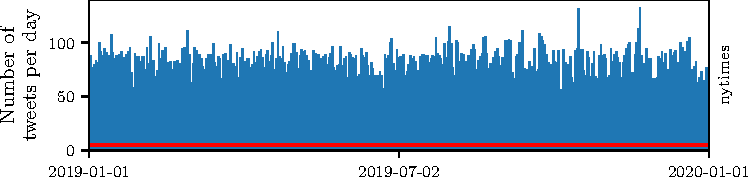
\includegraphics{appendix2/figs/tweet_times/nytimes.pdf}
	\captionof{figure}{Twitter activity over 2019 for `The New York Times'.
		Twitter handle is `nytimes' with 44800317 followers and 31029 total tweets in 2019. }
\end{center}



\begin{center}
	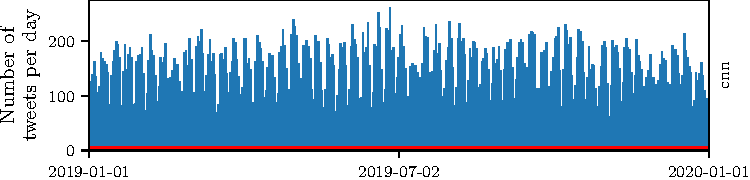
\includegraphics{appendix2/figs/tweet_times/cnn.pdf}
	\captionof{figure}{Twitter activity over 2019 for `CNN'.
		Twitter handle is `cnn' with 44153462 followers and 57155 total tweets in 2019. }
\end{center}



\begin{center}
	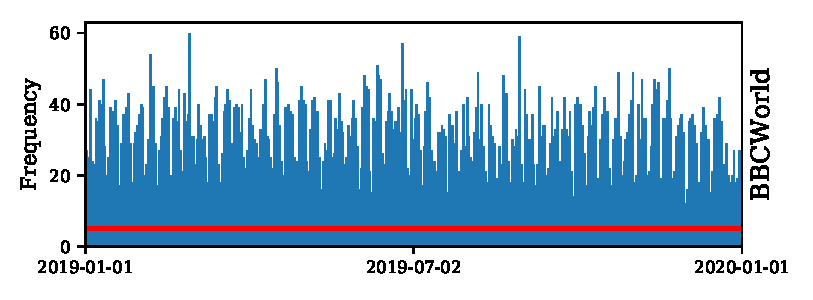
\includegraphics{appendix2/figs/tweet_times/BBCWorld.pdf}
	\captionof{figure}{Twitter activity over 2019 for `BBC News (World)'.
		Twitter handle is `BBCWorld' with 26446876 followers and 11679 total tweets in 2019. }
\end{center}



\begin{center}
	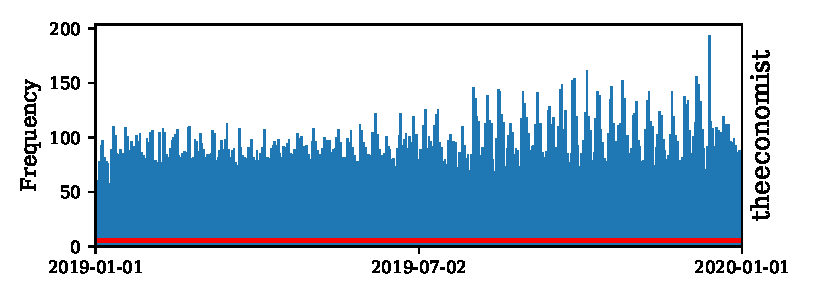
\includegraphics{appendix2/figs/tweet_times/theeconomist.pdf}
	\captionof{figure}{Twitter activity over 2019 for `The Economist'.
		Twitter handle is `theeconomist' with 24239639 followers and 35771 total tweets in 2019. }
\end{center}



\begin{center}
	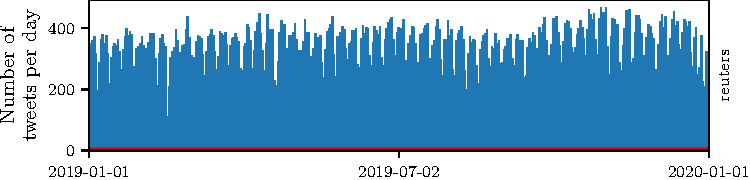
\includegraphics{appendix2/figs/tweet_times/reuters.pdf}
	\captionof{figure}{Twitter activity over 2019 for `Reuters'.
		Twitter handle is `reuters' with 21042215 followers and 128448 total tweets in 2019. }
\end{center}



\begin{center}
	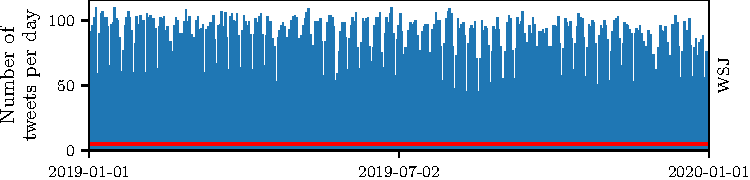
\includegraphics{appendix2/figs/tweet_times/WSJ.pdf}
	\captionof{figure}{Twitter activity over 2019 for `The Wall Street Journal'.
		Twitter handle is `WSJ' with 17139922 followers and 32151 total tweets in 2019. }
\end{center}



\begin{center}
	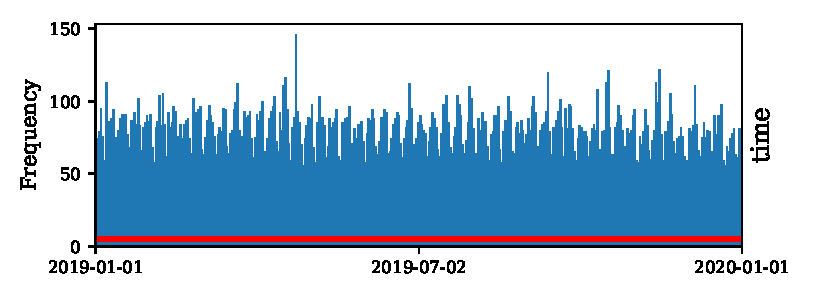
\includegraphics{appendix2/figs/tweet_times/time.pdf}
	\captionof{figure}{Twitter activity over 2019 for `TIME'.
		Twitter handle is `time' with 16512854 followers and 29631 total tweets in 2019. }
\end{center}



\begin{center}
	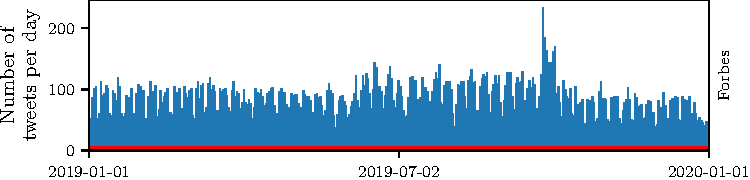
\includegraphics{appendix2/figs/tweet_times/Forbes.pdf}
	\captionof{figure}{Twitter activity over 2019 for `Forbes'.
		Twitter handle is `Forbes' with 15736852 followers and 31940 total tweets in 2019. }
\end{center}



\begin{center}
	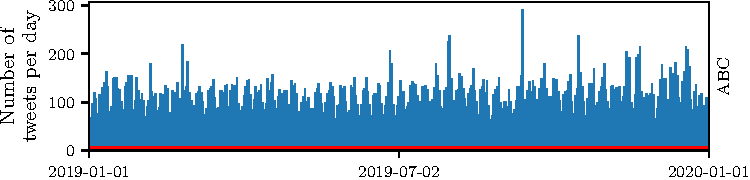
\includegraphics{appendix2/figs/tweet_times/ABC.pdf}
	\captionof{figure}{Twitter activity over 2019 for `ABC News'.
		Twitter handle is `ABC' with 14804638 followers and 44149 total tweets in 2019. }
\end{center}



\begin{center}
	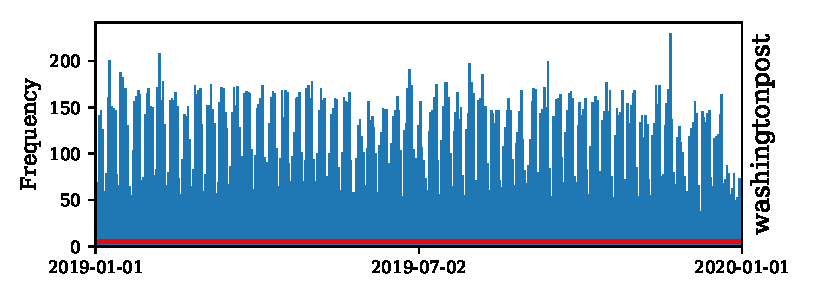
\includegraphics{appendix2/figs/tweet_times/washingtonpost.pdf}
	\captionof{figure}{Twitter activity over 2019 for `The Washington Post'.
		Twitter handle is `washingtonpost' with 14644580 followers and 45043 total tweets in 2019. }
\end{center}



\begin{center}
	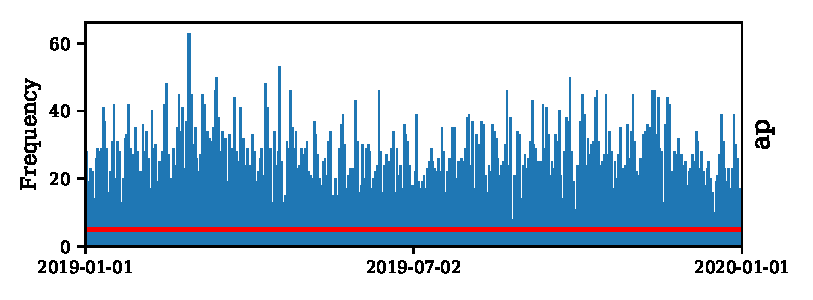
\includegraphics{appendix2/figs/tweet_times/ap.pdf}
	\captionof{figure}{Twitter activity over 2019 for `The Associated Press'.
		Twitter handle is `ap' with 13671750 followers and 10214 total tweets in 2019. }
\end{center}



\begin{center}
	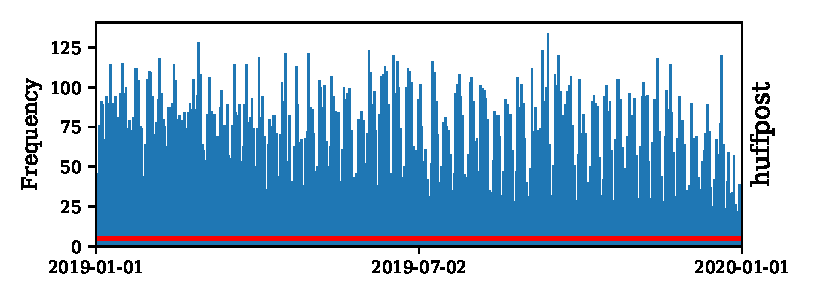
\includegraphics{appendix2/figs/tweet_times/huffpost.pdf}
	\captionof{figure}{Twitter activity over 2019 for `HuffPost'.
		Twitter handle is `huffpost' with 11472382 followers and 27622 total tweets in 2019. }
\end{center}



\begin{center}
	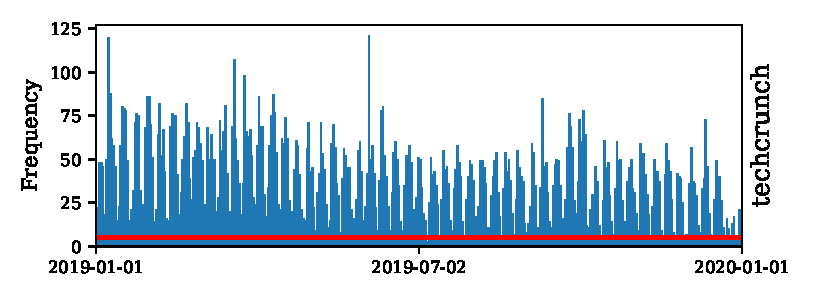
\includegraphics{appendix2/figs/tweet_times/techcrunch.pdf}
	\captionof{figure}{Twitter activity over 2019 for `TechCrunch'.
		Twitter handle is `techcrunch' with 10124437 followers and 14348 total tweets in 2019. }
\end{center}



\begin{center}
	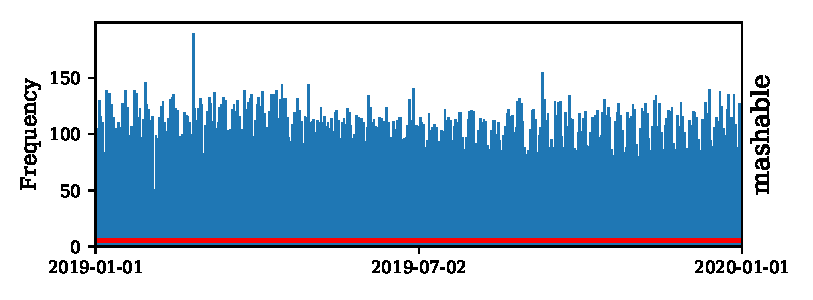
\includegraphics{appendix2/figs/tweet_times/mashable.pdf}
	\captionof{figure}{Twitter activity over 2019 for `Mashable'.
		Twitter handle is `mashable' with 9809420 followers and 40854 total tweets in 2019. }
\end{center}



\begin{center}
	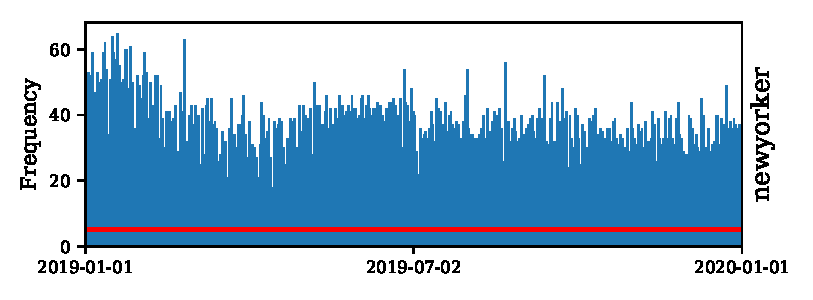
\includegraphics{appendix2/figs/tweet_times/newyorker.pdf}
	\captionof{figure}{Twitter activity over 2019 for `The New Yorker'.
		Twitter handle is `newyorker' with 8774527 followers and 13948 total tweets in 2019. }
\end{center}



\begin{center}
	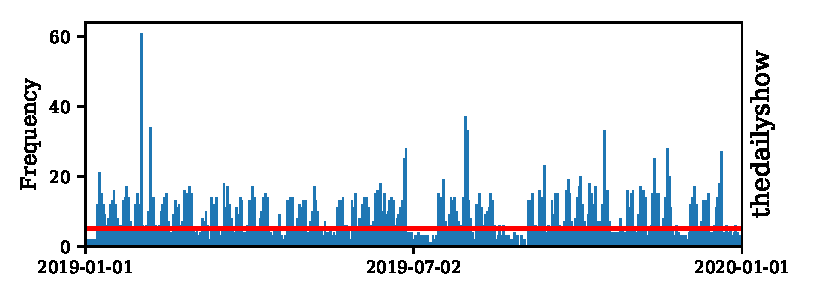
\includegraphics{appendix2/figs/tweet_times/thedailyshow.pdf}
	\captionof{figure}{Twitter activity over 2019 for `The Daily Show'.
		Twitter handle is `thedailyshow' with 8256511 followers and 3386 total tweets in 2019. }
\end{center}



\begin{center}
	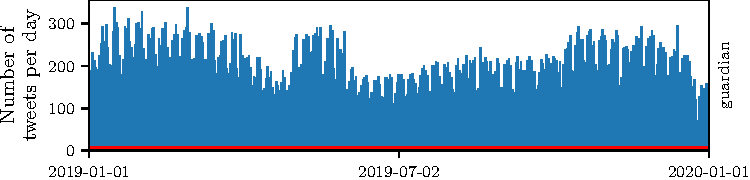
\includegraphics{appendix2/figs/tweet_times/guardian.pdf}
	\captionof{figure}{Twitter activity over 2019 for `The Guardian'.
		Twitter handle is `guardian' with 8243012 followers and 77532 total tweets in 2019. }
\end{center}



\begin{center}
	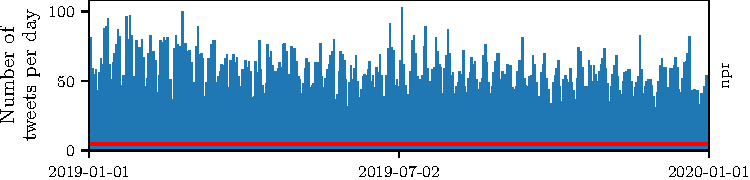
\includegraphics{appendix2/figs/tweet_times/npr.pdf}
	\captionof{figure}{Twitter activity over 2019 for `NPR'.
		Twitter handle is `npr' with 7959364 followers and 21236 total tweets in 2019. }
\end{center}



\begin{center}
	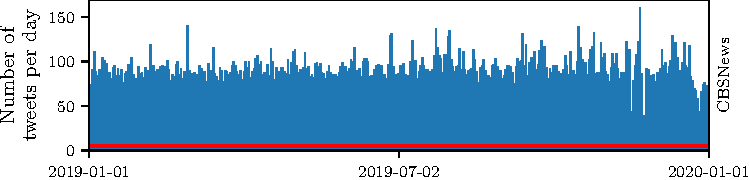
\includegraphics{appendix2/figs/tweet_times/CBSNews.pdf}
	\captionof{figure}{Twitter activity over 2019 for `CBS News'.
		Twitter handle is `CBSNews' with 7078950 followers and 34060 total tweets in 2019. }
\end{center}



\begin{center}
	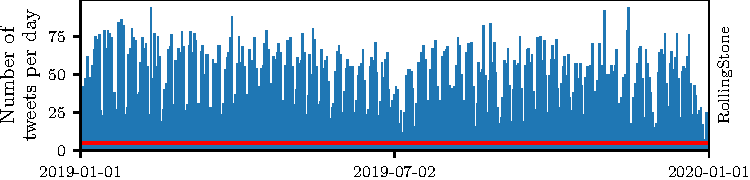
\includegraphics{appendix2/figs/tweet_times/RollingStone.pdf}
	\captionof{figure}{Twitter activity over 2019 for `Rolling Stone'.
		Twitter handle is `RollingStone' with 6295950 followers and 18571 total tweets in 2019. }
\end{center}



\begin{center}
	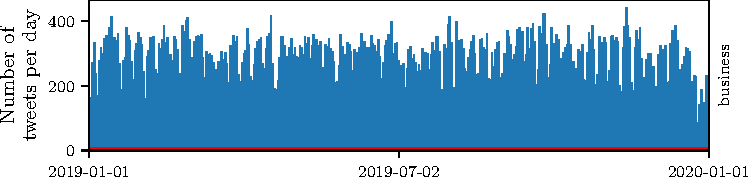
\includegraphics{appendix2/figs/tweet_times/business.pdf}
	\captionof{figure}{Twitter activity over 2019 for `Bloomberg'.
		Twitter handle is `business' with 5790419 followers and 109367 total tweets in 2019. }
\end{center}



\begin{center}
	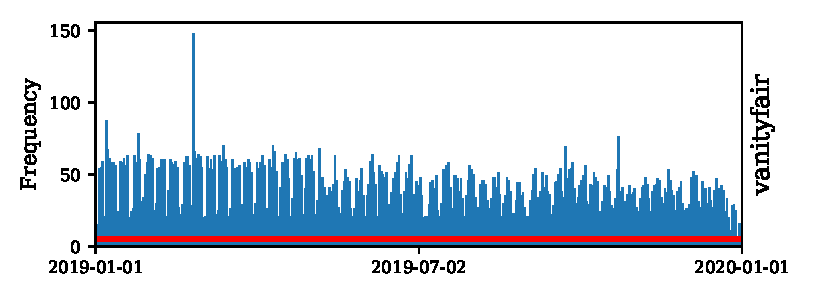
\includegraphics{appendix2/figs/tweet_times/vanityfair.pdf}
	\captionof{figure}{Twitter activity over 2019 for `VANITY FAIR'.
		Twitter handle is `vanityfair' with 4887894 followers and 15585 total tweets in 2019. }
\end{center}



\begin{center}
	\includegraphics{appendix2/figs/tweet_times/TODAYshow.pdf}
	\captionof{figure}{Twitter activity over 2019 for `TODAY'.
		Twitter handle is `TODAYshow' with 4282063 followers and 17678 total tweets in 2019. }
\end{center}



\begin{center}
	\includegraphics{appendix2/figs/tweet_times/lifehacker.pdf}
	\captionof{figure}{Twitter activity over 2019 for `Lifehacker'.
		Twitter handle is `lifehacker' with 4153410 followers and 9026 total tweets in 2019. }
\end{center}



\begin{center}
	\includegraphics{appendix2/figs/tweet_times/politico.pdf}
	\captionof{figure}{Twitter activity over 2019 for `POLITICO'.
		Twitter handle is `politico' with 4016243 followers and 25742 total tweets in 2019. }
\end{center}



\begin{center}
	\includegraphics{appendix2/figs/tweet_times/usatoday.pdf}
	\captionof{figure}{Twitter activity over 2019 for `USA TODAY'.
		Twitter handle is `usatoday' with 3949159 followers and 27303 total tweets in 2019. }
\end{center}



\begin{center}
	\includegraphics{appendix2/figs/tweet_times/FT.pdf}
	\captionof{figure}{Twitter activity over 2019 for `Financial Times'.
		Twitter handle is `FT' with 3806483 followers and 41030 total tweets in 2019. }
\end{center}



\begin{center}
	\includegraphics{appendix2/figs/tweet_times/sciam.pdf}
	\captionof{figure}{Twitter activity over 2019 for `Scientific American'.
		Twitter handle is `sciam' with 3805593 followers and 2335 total tweets in 2019. }
\end{center}



\begin{center}
	\includegraphics{appendix2/figs/tweet_times/thehill.pdf}
	\captionof{figure}{Twitter activity over 2019 for `The Hill'.
		Twitter handle is `thehill' with 3501890 followers and 157172 total tweets in 2019. }
\end{center}



\begin{center}
	\includegraphics{appendix2/figs/tweet_times/latimes.pdf}
	\captionof{figure}{Twitter activity over 2019 for `Los Angeles Times'.
		Twitter handle is `latimes' with 3473994 followers and 35341 total tweets in 2019. }
\end{center}



\begin{center}
	\includegraphics{appendix2/figs/tweet_times/newsweek.pdf}
	\captionof{figure}{Twitter activity over 2019 for `Newsweek'.
		Twitter handle is `newsweek' with 3407905 followers and 46922 total tweets in 2019. }
\end{center}



\begin{center}
	\includegraphics{appendix2/figs/tweet_times/TeenVogue.pdf}
	\captionof{figure}{Twitter activity over 2019 for `Teen Vogue'.
		Twitter handle is `TeenVogue' with 3358001 followers and 12270 total tweets in 2019. }
\end{center}



\begin{center}
	\includegraphics{appendix2/figs/tweet_times/cnbc.pdf}
	\captionof{figure}{Twitter activity over 2019 for `CNBC'.
		Twitter handle is `cnbc' with 3355408 followers and 66578 total tweets in 2019. }
\end{center}



\begin{center}
	\includegraphics{appendix2/figs/tweet_times/msnbc.pdf}
	\captionof{figure}{Twitter activity over 2019 for `MSNBC'.
		Twitter handle is `msnbc' with 2870702 followers and 32699 total tweets in 2019. }
\end{center}



\begin{center}
	\includegraphics{appendix2/figs/tweet_times/businessinsider.pdf}
	\captionof{figure}{Twitter activity over 2019 for `Business Insider'.
		Twitter handle is `businessinsider' with 2790009 followers and 57915 total tweets in 2019. }
\end{center}



\begin{center}
	\includegraphics{appendix2/figs/tweet_times/Telegraph.pdf}
	\captionof{figure}{Twitter activity over 2019 for `The Telegraph'.
		Twitter handle is `Telegraph' with 2774439 followers and 24235 total tweets in 2019. }
\end{center}



\begin{center}
	\includegraphics{appendix2/figs/tweet_times/verge.pdf}
	\captionof{figure}{Twitter activity over 2019 for `The Verge'.
		Twitter handle is `verge' with 2613577 followers and 19096 total tweets in 2019. }
\end{center}



\begin{center}
	\includegraphics{appendix2/figs/tweet_times/MailOnline.pdf}
	\captionof{figure}{Twitter activity over 2019 for `Daily Mail Online'.
		Twitter handle is `MailOnline' with 2437611 followers and 28671 total tweets in 2019. }
\end{center}



\begin{center}
	\includegraphics{appendix2/figs/tweet_times/vice.pdf}
	\captionof{figure}{Twitter activity over 2019 for `VICE'.
		Twitter handle is `vice' with 2000034 followers and 17195 total tweets in 2019. }
\end{center}



\begin{center}
	\includegraphics{appendix2/figs/tweet_times/cspan.pdf}
	\captionof{figure}{Twitter activity over 2019 for `CSPAN'.
		Twitter handle is `cspan' with 1989017 followers and 5022 total tweets in 2019. }
\end{center}



\begin{center}
	\includegraphics{appendix2/figs/tweet_times/theatlantic.pdf}
	\captionof{figure}{Twitter activity over 2019 for `The Atlantic'.
		Twitter handle is `theatlantic' with 1850164 followers and 15100 total tweets in 2019. }
\end{center}



\begin{center}
	\includegraphics{appendix2/figs/tweet_times/NYMag.pdf}
	\captionof{figure}{Twitter activity over 2019 for `New York Magazine'.
		Twitter handle is `NYMag' with 1800255 followers and 19072 total tweets in 2019. }
\end{center}



\begin{center}
	\includegraphics{appendix2/figs/tweet_times/slate.pdf}
	\captionof{figure}{Twitter activity over 2019 for `Slate'.
		Twitter handle is `slate' with 1792093 followers and 58598 total tweets in 2019. }
\end{center}



\begin{center}
	\includegraphics{appendix2/figs/tweet_times/AJENews.pdf}
	\captionof{figure}{Twitter activity over 2019 for `Al Jazeera News'.
		Twitter handle is `AJENews' with 1573047 followers and 11252 total tweets in 2019. }
\end{center}



\begin{center}
	\includegraphics{appendix2/figs/tweet_times/nypost.pdf}
	\captionof{figure}{Twitter activity over 2019 for `New York Post'.
		Twitter handle is `nypost' with 1543609 followers and 79771 total tweets in 2019. }
\end{center}



\begin{center}
	\includegraphics{appendix2/figs/tweet_times/BuzzFeedNews.pdf}
	\captionof{figure}{Twitter activity over 2019 for `BuzzFeed News'.
		Twitter handle is `BuzzFeedNews' with 1338555 followers and 19705 total tweets in 2019. }
\end{center}



\begin{center}
	\includegraphics{appendix2/figs/tweet_times/BreitbartNews.pdf}
	\captionof{figure}{Twitter activity over 2019 for `Breitbart News'.
		Twitter handle is `BreitbartNews' with 1225203 followers and 17501 total tweets in 2019. }
\end{center}



\begin{center}
	\includegraphics{appendix2/figs/tweet_times/YahooNews.pdf}
	\captionof{figure}{Twitter activity over 2019 for `Yahoo News'.
		Twitter handle is `YahooNews' with 1106092 followers and 19781 total tweets in 2019. }
\end{center}



\begin{center}
	\includegraphics{appendix2/figs/tweet_times/chicagotribune.pdf}
	\captionof{figure}{Twitter activity over 2019 for `Chicago Tribune'.
		Twitter handle is `chicagotribune' with 1099101 followers and 22994 total tweets in 2019. }
\end{center}



\begin{center}
	\includegraphics{appendix2/figs/tweet_times/ajc.pdf}
	\captionof{figure}{Twitter activity over 2019 for `AJC'.
		Twitter handle is `ajc' with 1045546 followers and 27978 total tweets in 2019. }
\end{center}



\begin{center}
	\includegraphics{appendix2/figs/tweet_times/NewsHour.pdf}
	\captionof{figure}{Twitter activity over 2019 for `PBS NewsHour'.
		Twitter handle is `NewsHour' with 1036993 followers and 16189 total tweets in 2019. }
\end{center}



\begin{center}
	\includegraphics{appendix2/figs/tweet_times/salon.pdf}
	\captionof{figure}{Twitter activity over 2019 for `Salon'.
		Twitter handle is `salon' with 976078 followers and 11614 total tweets in 2019. }
\end{center}



\begin{center}
	\includegraphics{appendix2/figs/tweet_times/voxdotcom.pdf}
	\captionof{figure}{Twitter activity over 2019 for `Vox'.
		Twitter handle is `voxdotcom' with 891290 followers and 17574 total tweets in 2019. }
\end{center}



\begin{center}
	\includegraphics{appendix2/figs/tweet_times/propublica.pdf}
	\captionof{figure}{Twitter activity over 2019 for `ProPublica'.
		Twitter handle is `propublica' with 833038 followers and 6458 total tweets in 2019. }
\end{center}



\begin{center}
	\includegraphics{appendix2/figs/tweet_times/motherjones.pdf}
	\captionof{figure}{Twitter activity over 2019 for `Mother Jones'.
		Twitter handle is `motherjones' with 809121 followers and 16447 total tweets in 2019. }
\end{center}



\begin{center}
	\includegraphics{appendix2/figs/tweet_times/bostonglobe.pdf}
	\captionof{figure}{Twitter activity over 2019 for `The Boston Globe'.
		Twitter handle is `bostonglobe' with 756522 followers and 49224 total tweets in 2019. }
\end{center}



\begin{center}
	\includegraphics{appendix2/figs/tweet_times/theintercept.pdf}
	\captionof{figure}{Twitter activity over 2019 for `The Intercept'.
		Twitter handle is `theintercept' with 753001 followers and 6642 total tweets in 2019. }
\end{center}



\begin{center}
	\includegraphics{appendix2/figs/tweet_times/nydailynews.pdf}
	\captionof{figure}{Twitter activity over 2019 for `New York Daily News'.
		Twitter handle is `nydailynews' with 728512 followers and 28682 total tweets in 2019. }
\end{center}



\begin{center}
	\includegraphics{appendix2/figs/tweet_times/ForeignAffairs.pdf}
	\captionof{figure}{Twitter activity over 2019 for `Foreign Affairs'.
		Twitter handle is `ForeignAffairs' with 724994 followers and 11964 total tweets in 2019. }
\end{center}



\begin{center}
	\includegraphics{appendix2/figs/tweet_times/nytopinion.pdf}
	\captionof{figure}{Twitter activity over 2019 for `New York Times Opinion'.
		Twitter handle is `nytopinion' with 718663 followers and 25402 total tweets in 2019. }
\end{center}



\begin{center}
	\includegraphics{appendix2/figs/tweet_times/democracynow.pdf}
	\captionof{figure}{Twitter activity over 2019 for `Democracy Now!'.
		Twitter handle is `democracynow' with 710714 followers and 9453 total tweets in 2019. }
\end{center}



\begin{center}
	\includegraphics{appendix2/figs/tweet_times/theblaze.pdf}
	\captionof{figure}{Twitter activity over 2019 for `TheBlaze'.
		Twitter handle is `theblaze' with 706991 followers and 13121 total tweets in 2019. }
\end{center}



\begin{center}
	\includegraphics{appendix2/figs/tweet_times/DailyCaller.pdf}
	\captionof{figure}{Twitter activity over 2019 for `Daily Caller'.
		Twitter handle is `DailyCaller' with 579741 followers and 34716 total tweets in 2019. }
\end{center}



\begin{center}
	\includegraphics{appendix2/figs/tweet_times/TheRoot.pdf}
	\captionof{figure}{Twitter activity over 2019 for `The Root'.
		Twitter handle is `TheRoot' with 525879 followers and 6994 total tweets in 2019. }
\end{center}



\begin{center}
	\includegraphics{appendix2/figs/tweet_times/upworthy.pdf}
	\captionof{figure}{Twitter activity over 2019 for `Upworthy'.
		Twitter handle is `upworthy' with 511090 followers and 1472 total tweets in 2019. }
\end{center}



\begin{center}
	\includegraphics{appendix2/figs/tweet_times/OANN.pdf}
	\captionof{figure}{Twitter activity over 2019 for `One America News'.
		Twitter handle is `OANN' with 510392 followers and 6108 total tweets in 2019. }
\end{center}



\begin{center}
	\includegraphics{appendix2/figs/tweet_times/Suntimes.pdf}
	\captionof{figure}{Twitter activity over 2019 for `Chicago Sun-Times'.
		Twitter handle is `Suntimes' with 505161 followers and 15976 total tweets in 2019. }
\end{center}



\begin{center}
	\includegraphics{appendix2/figs/tweet_times/sfgate.pdf}
	\captionof{figure}{Twitter activity over 2019 for `SFGate'.
		Twitter handle is `sfgate' with 477782 followers and 17838 total tweets in 2019. }
\end{center}



\begin{center}
	\includegraphics{appendix2/figs/tweet_times/MiamiHerald.pdf}
	\captionof{figure}{Twitter activity over 2019 for `Miami Herald'.
		Twitter handle is `MiamiHerald' with 450869 followers and 19290 total tweets in 2019. }
\end{center}



\begin{center}
	\includegraphics{appendix2/figs/tweet_times/Jerusalem_Post.pdf}
	\captionof{figure}{Twitter activity over 2019 for `The Jerusalem Post'.
		Twitter handle is `Jerusalem\_Post' with 445004 followers and 29868 total tweets in 2019. }
\end{center}



\begin{center}
	\includegraphics{appendix2/figs/tweet_times/esquire.pdf}
	\captionof{figure}{Twitter activity over 2019 for `Esquire'.
		Twitter handle is `esquire' with 418881 followers and 12817 total tweets in 2019. }
\end{center}



\begin{center}
	\includegraphics{appendix2/figs/tweet_times/qz.pdf}
	\captionof{figure}{Twitter activity over 2019 for `Quartz'.
		Twitter handle is `qz' with 384220 followers and 28604 total tweets in 2019. }
\end{center}



\begin{center}
	\includegraphics{appendix2/figs/tweet_times/WashTimes.pdf}
	\captionof{figure}{Twitter activity over 2019 for `The Washington Times'.
		Twitter handle is `WashTimes' with 372421 followers and 34635 total tweets in 2019. }
\end{center}



\begin{center}
	\includegraphics{appendix2/figs/tweet_times/rollcall.pdf}
	\captionof{figure}{Twitter activity over 2019 for `Roll Call'.
		Twitter handle is `rollcall' with 361580 followers and 10157 total tweets in 2019. }
\end{center}



\begin{center}
	\includegraphics{appendix2/figs/tweet_times/realdailywire.pdf}
	\captionof{figure}{Twitter activity over 2019 for `The Daily Wire'.
		Twitter handle is `realdailywire' with 361505 followers and 26385 total tweets in 2019. }
\end{center}



\begin{center}
	\includegraphics{appendix2/figs/tweet_times/NRO.pdf}
	\captionof{figure}{Twitter activity over 2019 for `National Review'.
		Twitter handle is `NRO' with 336300 followers and 16572 total tweets in 2019. }
\end{center}



\begin{center}
	\includegraphics{appendix2/figs/tweet_times/axios.pdf}
	\captionof{figure}{Twitter activity over 2019 for `Axios'.
		Twitter handle is `axios' with 315533 followers and 19184 total tweets in 2019. }
\end{center}



\begin{center}
	\includegraphics{appendix2/figs/tweet_times/statesman.pdf}
	\captionof{figure}{Twitter activity over 2019 for `Austin Statesman'.
		Twitter handle is `statesman' with 300429 followers and 9562 total tweets in 2019. }
\end{center}



\begin{center}
	\includegraphics{appendix2/figs/tweet_times/dailykos.pdf}
	\captionof{figure}{Twitter activity over 2019 for `Daily Kos'.
		Twitter handle is `dailykos' with 280636 followers and 12636 total tweets in 2019. }
\end{center}



\begin{center}
	\includegraphics{appendix2/figs/tweet_times/reason.pdf}
	\captionof{figure}{Twitter activity over 2019 for `reason'.
		Twitter handle is `reason' with 242262 followers and 7939 total tweets in 2019. }
\end{center}



\begin{center}
	\includegraphics{appendix2/figs/tweet_times/mercnews.pdf}
	\captionof{figure}{Twitter activity over 2019 for `Mercury News'.
		Twitter handle is `mercnews' with 241228 followers and 36535 total tweets in 2019. }
\end{center}



\begin{center}
	\includegraphics{appendix2/figs/tweet_times/jacobinmag.pdf}
	\captionof{figure}{Twitter activity over 2019 for `Jacobin'.
		Twitter handle is `jacobinmag' with 241092 followers and 8579 total tweets in 2019. }
\end{center}



\begin{center}
	\includegraphics{appendix2/figs/tweet_times/sciencedaily.pdf}
	\captionof{figure}{Twitter activity over 2019 for `ScienceDaily'.
		Twitter handle is `sciencedaily' with 240013 followers and 1243 total tweets in 2019. }
\end{center}



\begin{center}
	\includegraphics{appendix2/figs/tweet_times/LasVegasSun.pdf}
	\captionof{figure}{Twitter activity over 2019 for `Las Vegas Sun'.
		Twitter handle is `LasVegasSun' with 238797 followers and 8233 total tweets in 2019. }
\end{center}



\begin{center}
	\includegraphics{appendix2/figs/tweet_times/grist.pdf}
	\captionof{figure}{Twitter activity over 2019 for `grist'.
		Twitter handle is `grist' with 230344 followers and 6438 total tweets in 2019. }
\end{center}



\begin{center}
	\includegraphics{appendix2/figs/tweet_times/sacbee_news.pdf}
	\captionof{figure}{Twitter activity over 2019 for `The Sacramento Bee'.
		Twitter handle is `sacbee\_news' with 219066 followers and 22511 total tweets in 2019. }
\end{center}



\begin{center}
	\includegraphics{appendix2/figs/tweet_times/redstate.pdf}
	\captionof{figure}{Twitter activity over 2019 for `RedState'.
		Twitter handle is `redstate' with 218545 followers and 19778 total tweets in 2019. }
\end{center}



\begin{center}
	\includegraphics{appendix2/figs/tweet_times/FDRLST.pdf}
	\captionof{figure}{Twitter activity over 2019 for `The Federalist'.
		Twitter handle is `FDRLST' with 217053 followers and 5830 total tweets in 2019. }
\end{center}



\begin{center}
	\includegraphics{appendix2/figs/tweet_times/ocregister.pdf}
	\captionof{figure}{Twitter activity over 2019 for `O.C. Register'.
		Twitter handle is `ocregister' with 212517 followers and 23872 total tweets in 2019. }
\end{center}



\begin{center}
	\includegraphics{appendix2/figs/tweet_times/sfweekly.pdf}
	\captionof{figure}{Twitter activity over 2019 for `SF Weekly'.
		Twitter handle is `sfweekly' with 210524 followers and 4438 total tweets in 2019. }
\end{center}



\begin{center}
	\includegraphics{appendix2/figs/tweet_times/rawstory.pdf}
	\captionof{figure}{Twitter activity over 2019 for `Raw Story'.
		Twitter handle is `rawstory' with 205992 followers and 29702 total tweets in 2019. }
\end{center}



\begin{center}
	\includegraphics{appendix2/figs/tweet_times/dcexaminer.pdf}
	\captionof{figure}{Twitter activity over 2019 for `Washington Examiner'.
		Twitter handle is `dcexaminer' with 198229 followers and 61833 total tweets in 2019. }
\end{center}



\begin{center}
	\includegraphics{appendix2/figs/tweet_times/observer.pdf}
	\captionof{figure}{Twitter activity over 2019 for `OBSERVER'.
		Twitter handle is `observer' with 195067 followers and 5856 total tweets in 2019. }
\end{center}



\begin{center}
	\includegraphics{appendix2/figs/tweet_times/sfchronicle.pdf}
	\captionof{figure}{Twitter activity over 2019 for `San Francisco Chronicle'.
		Twitter handle is `sfchronicle' with 189685 followers and 18021 total tweets in 2019. }
\end{center}



\begin{center}
	\includegraphics{appendix2/figs/tweet_times/KSLcom.pdf}
	\captionof{figure}{Twitter activity over 2019 for `KSL'.
		Twitter handle is `KSLcom' with 179424 followers and 11881 total tweets in 2019. }
\end{center}



\begin{center}
	\includegraphics{appendix2/figs/tweet_times/truthout.pdf}
	\captionof{figure}{Twitter activity over 2019 for `Truthout'.
		Twitter handle is `truthout' with 170572 followers and 7806 total tweets in 2019. }
\end{center}



\begin{center}
	\includegraphics{appendix2/figs/tweet_times/newrepublic.pdf}
	\captionof{figure}{Twitter activity over 2019 for `The New Republic'.
		Twitter handle is `newrepublic' with 167916 followers and 10725 total tweets in 2019. }
\end{center}



\begin{center}
	\includegraphics{appendix2/figs/tweet_times/IBDinvestors.pdf}
	\captionof{figure}{Twitter activity over 2019 for `Investors.com'.
		Twitter handle is `IBDinvestors' with 167242 followers and 2469 total tweets in 2019. }
\end{center}



\begin{center}
	\includegraphics{appendix2/figs/tweet_times/PittsburghPG.pdf}
	\captionof{figure}{Twitter activity over 2019 for `Pittsburgh Post-Gazette'.
		Twitter handle is `PittsburghPG' with 166684 followers and 24711 total tweets in 2019. }
\end{center}



\begin{center}
	\includegraphics{appendix2/figs/tweet_times/memphisnews.pdf}
	\captionof{figure}{Twitter activity over 2019 for `Commercial Appeal'.
		Twitter handle is `memphisnews' with 162002 followers and 15885 total tweets in 2019. }
\end{center}



\begin{center}
	\includegraphics{appendix2/figs/tweet_times/Mediaite.pdf}
	\captionof{figure}{Twitter activity over 2019 for `Mediaite'.
		Twitter handle is `Mediaite' with 159980 followers and 14030 total tweets in 2019. }
\end{center}



\begin{center}
	\includegraphics{appendix2/figs/tweet_times/townhallcom.pdf}
	\captionof{figure}{Twitter activity over 2019 for `Townhall.com'.
		Twitter handle is `townhallcom' with 152082 followers and 10452 total tweets in 2019. }
\end{center}



\begin{center}
	\includegraphics{appendix2/figs/tweet_times/usnews.pdf}
	\captionof{figure}{Twitter activity over 2019 for `U.S. News'.
		Twitter handle is `usnews' with 150674 followers and 12827 total tweets in 2019. }
\end{center}



\begin{center}
	\includegraphics{appendix2/figs/tweet_times/alternet.pdf}
	\captionof{figure}{Twitter activity over 2019 for `AlterNet'.
		Twitter handle is `alternet' with 139194 followers and 7156 total tweets in 2019. }
\end{center}



\begin{center}
	\includegraphics{appendix2/figs/tweet_times/nationaljournal.pdf}
	\captionof{figure}{Twitter activity over 2019 for `National Journal'.
		Twitter handle is `nationaljournal' with 133097 followers and 1424 total tweets in 2019. }
\end{center}



\begin{center}
	\includegraphics{appendix2/figs/tweet_times/theweek.pdf}
	\captionof{figure}{Twitter activity over 2019 for `The Week'.
		Twitter handle is `theweek' with 129703 followers and 9031 total tweets in 2019. }
\end{center}



\begin{center}
	\includegraphics{appendix2/figs/tweet_times/CBNNews.pdf}
	\captionof{figure}{Twitter activity over 2019 for `CBN News'.
		Twitter handle is `CBNNews' with 128487 followers and 15627 total tweets in 2019. }
\end{center}



\begin{center}
	\includegraphics{appendix2/figs/tweet_times/IBTimes.pdf}
	\captionof{figure}{Twitter activity over 2019 for `Intl. Business Times'.
		Twitter handle is `IBTimes' with 123358 followers and 11519 total tweets in 2019. }
\end{center}



\begin{center}
	\includegraphics{appendix2/figs/tweet_times/cnsnews.pdf}
	\captionof{figure}{Twitter activity over 2019 for `CNSNews.com'.
		Twitter handle is `cnsnews' with 119236 followers and 9035 total tweets in 2019. }
\end{center}



\begin{center}
	\includegraphics{appendix2/figs/tweet_times/RTDNEWS.pdf}
	\captionof{figure}{Twitter activity over 2019 for `Times-Dispatch'.
		Twitter handle is `RTDNEWS' with 116510 followers and 7018 total tweets in 2019. }
\end{center}



\begin{center}
	\includegraphics{appendix2/figs/tweet_times/FreeBeacon.pdf}
	\captionof{figure}{Twitter activity over 2019 for `Free Beacon'.
		Twitter handle is `FreeBeacon' with 110634 followers and 9091 total tweets in 2019. }
\end{center}



\begin{center}
	\includegraphics{appendix2/figs/tweet_times/bostonherald.pdf}
	\captionof{figure}{Twitter activity over 2019 for `Boston Herald'.
		Twitter handle is `bostonherald' with 105046 followers and 12550 total tweets in 2019. }
\end{center}



\begin{center}
	\includegraphics{appendix2/figs/tweet_times/newsmax.pdf}
	\captionof{figure}{Twitter activity over 2019 for `Newsmax'.
		Twitter handle is `newsmax' with 100437 followers and 3825 total tweets in 2019. }
\end{center}



\begin{center}
	\includegraphics{appendix2/figs/tweet_times/curaffairs.pdf}
	\captionof{figure}{Twitter activity over 2019 for `Current Affairs'.
		Twitter handle is `curaffairs' with 99136 followers and 2188 total tweets in 2019. }
\end{center}



\begin{center}
	\includegraphics{appendix2/figs/tweet_times/DeseretNews.pdf}
	\captionof{figure}{Twitter activity over 2019 for `Deseret News'.
		Twitter handle is `DeseretNews' with 97060 followers and 15087 total tweets in 2019. }
\end{center}



\begin{center}
	\includegraphics{appendix2/figs/tweet_times/WSJopinion.pdf}
	\captionof{figure}{Twitter activity over 2019 for `WSJ Editorial Page'.
		Twitter handle is `WSJopinion' with 96734 followers and 4990 total tweets in 2019. }
\end{center}



\begin{center}
	\includegraphics{appendix2/figs/tweet_times/bustle.pdf}
	\captionof{figure}{Twitter activity over 2019 for `Bustle'.
		Twitter handle is `bustle' with 96170 followers and 1504 total tweets in 2019. }
\end{center}



\begin{center}
	\includegraphics{appendix2/figs/tweet_times/courierjournal.pdf}
	\captionof{figure}{Twitter activity over 2019 for `Courier Journal'.
		Twitter handle is `courierjournal' with 88551 followers and 13988 total tweets in 2019. }
\end{center}



\begin{center}
	\includegraphics{appendix2/figs/tweet_times/PressHerald.pdf}
	\captionof{figure}{Twitter activity over 2019 for `Portland Press Herald'.
		Twitter handle is `PressHerald' with 85834 followers and 6372 total tweets in 2019. }
\end{center}



\begin{center}
	\includegraphics{appendix2/figs/tweet_times/DefenseOne.pdf}
	\captionof{figure}{Twitter activity over 2019 for `Defense One'.
		Twitter handle is `DefenseOne' with 81992 followers and 6892 total tweets in 2019. }
\end{center}



\begin{center}
	\includegraphics{appendix2/figs/tweet_times/The_Nation.pdf}
	\captionof{figure}{Twitter activity over 2019 for `The Nation'.
		Twitter handle is `The\_Nation' with 78860 followers and 13048 total tweets in 2019. }
\end{center}



\begin{center}
	\includegraphics{appendix2/figs/tweet_times/csmonitor.pdf}
	\captionof{figure}{Twitter activity over 2019 for `The Christian Science Monitor'.
		Twitter handle is `csmonitor' with 75406 followers and 5676 total tweets in 2019. }
\end{center}



\begin{center}
	\includegraphics{appendix2/figs/tweet_times/ArkansasOnline.pdf}
	\captionof{figure}{Twitter activity over 2019 for `AR Democrat-Gazette'.
		Twitter handle is `ArkansasOnline' with 74177 followers and 10951 total tweets in 2019. }
\end{center}



\begin{center}
	\includegraphics{appendix2/figs/tweet_times/indyweek.pdf}
	\captionof{figure}{Twitter activity over 2019 for `INDY Week'.
		Twitter handle is `indyweek' with 73802 followers and 4175 total tweets in 2019. }
\end{center}



\begin{center}
	\includegraphics{appendix2/figs/tweet_times/PoliticusUSA.pdf}
	\captionof{figure}{Twitter activity over 2019 for `PoliticusUSA'.
		Twitter handle is `PoliticusUSA' with 72856 followers and 7253 total tweets in 2019. }
\end{center}



\begin{center}
	\includegraphics{appendix2/figs/tweet_times/Dailysignal.pdf}
	\captionof{figure}{Twitter activity over 2019 for `The Daily Signal'.
		Twitter handle is `Dailysignal' with 68024 followers and 6740 total tweets in 2019. }
\end{center}



\begin{center}
	\includegraphics{appendix2/figs/tweet_times/PJMedia_com.pdf}
	\captionof{figure}{Twitter activity over 2019 for `PJ Media'.
		Twitter handle is `PJMedia\_com' with 66324 followers and 5666 total tweets in 2019. }
\end{center}



\begin{center}
	\includegraphics{appendix2/figs/tweet_times/delcotimes.pdf}
	\captionof{figure}{Twitter activity over 2019 for `Delco Times'.
		Twitter handle is `delcotimes' with 64714 followers and 3302 total tweets in 2019. }
\end{center}



\begin{center}
	\includegraphics{appendix2/figs/tweet_times/Daily_Press.pdf}
	\captionof{figure}{Twitter activity over 2019 for `Daily Press'.
		Twitter handle is `Daily\_Press' with 61225 followers and 3512 total tweets in 2019. }
\end{center}



\begin{center}
	\includegraphics{appendix2/figs/tweet_times/yesmagazine.pdf}
	\captionof{figure}{Twitter activity over 2019 for `YES! Magazine'.
		Twitter handle is `yesmagazine' with 60455 followers and 4679 total tweets in 2019. }
\end{center}



\begin{center}
	\includegraphics{appendix2/figs/tweet_times/SpokesmanReview.pdf}
	\captionof{figure}{Twitter activity over 2019 for `SpokesmanReview'.
		Twitter handle is `SpokesmanReview' with 58352 followers and 4113 total tweets in 2019. }
\end{center}



\begin{center}
	\includegraphics{appendix2/figs/tweet_times/TDOnline.pdf}
	\captionof{figure}{Twitter activity over 2019 for `Tallahassee Democrat'.
		Twitter handle is `TDOnline' with 53700 followers and 15098 total tweets in 2019. }
\end{center}



\begin{center}
	\includegraphics{appendix2/figs/tweet_times/TheKoreaHerald.pdf}
	\captionof{figure}{Twitter activity over 2019 for `The Korea Herald'.
		Twitter handle is `TheKoreaHerald' with 53517 followers and 8730 total tweets in 2019. }
\end{center}



\begin{center}
	\includegraphics{appendix2/figs/tweet_times/michigandaily.pdf}
	\captionof{figure}{Twitter activity over 2019 for `The Michigan Daily'.
		Twitter handle is `michigandaily' with 50748 followers and 2041 total tweets in 2019. }
\end{center}



\begin{center}
	\includegraphics{appendix2/figs/tweet_times/CivilBeat.pdf}
	\captionof{figure}{Twitter activity over 2019 for `Honolulu Civil Beat'.
		Twitter handle is `CivilBeat' with 50503 followers and 1837 total tweets in 2019. }
\end{center}



\begin{center}
	\includegraphics{appendix2/figs/tweet_times/TheLibRepublic.pdf}
	\captionof{figure}{Twitter activity over 2019 for `Libertarian Republic'.
		Twitter handle is `TheLibRepublic' with 47475 followers and 1145 total tweets in 2019. }
\end{center}



\begin{center}
	\includegraphics{appendix2/figs/tweet_times/amconmag.pdf}
	\captionof{figure}{Twitter activity over 2019 for `The American Conservative'.
		Twitter handle is `amconmag' with 46189 followers and 25197 total tweets in 2019. }
\end{center}



\begin{center}
	\includegraphics{appendix2/figs/tweet_times/amspectator.pdf}
	\captionof{figure}{Twitter activity over 2019 for `The American Spectator'.
		Twitter handle is `amspectator' with 45877 followers and 1915 total tweets in 2019. }
\end{center}



\begin{center}
	\includegraphics{appendix2/figs/tweet_times/redandblack.pdf}
	\captionof{figure}{Twitter activity over 2019 for `The Red \& Black'.
		Twitter handle is `redandblack' with 42735 followers and 7663 total tweets in 2019. }
\end{center}



\begin{center}
	\includegraphics{appendix2/figs/tweet_times/kqednews.pdf}
	\captionof{figure}{Twitter activity over 2019 for `KQED News'.
		Twitter handle is `kqednews' with 41720 followers and 8655 total tweets in 2019. }
\end{center}



\begin{center}
	\includegraphics{appendix2/figs/tweet_times/idsnews.pdf}
	\captionof{figure}{Twitter activity over 2019 for `Indiana Daily Student'.
		Twitter handle is `idsnews' with 41621 followers and 3867 total tweets in 2019. }
\end{center}



\begin{center}
	\includegraphics{appendix2/figs/tweet_times/wgbh.pdf}
	\captionof{figure}{Twitter activity over 2019 for `WGBH'.
		Twitter handle is `wgbh' with 39971 followers and 2211 total tweets in 2019. }
\end{center}



\begin{center}
	\includegraphics{appendix2/figs/tweet_times/WestJournalism.pdf}
	\captionof{figure}{Twitter activity over 2019 for `The Western Journal'.
		Twitter handle is `WestJournalism' with 38478 followers and 7114 total tweets in 2019. }
\end{center}



\begin{center}
	\includegraphics{appendix2/figs/tweet_times/Commentary.pdf}
	\captionof{figure}{Twitter activity over 2019 for `Commentary Magazine'.
		Twitter handle is `Commentary' with 35704 followers and 1337 total tweets in 2019. }
\end{center}



\begin{center}
	\includegraphics{appendix2/figs/tweet_times/DailyProgress.pdf}
	\captionof{figure}{Twitter activity over 2019 for `The Daily Progress'.
		Twitter handle is `DailyProgress' with 35506 followers and 6856 total tweets in 2019. }
\end{center}



\begin{center}
	\includegraphics{appendix2/figs/tweet_times/vtdigger.pdf}
	\captionof{figure}{Twitter activity over 2019 for `VTDigger'.
		Twitter handle is `vtdigger' with 32820 followers and 5671 total tweets in 2019. }
\end{center}



\begin{center}
	\includegraphics{appendix2/figs/tweet_times/bgdailynews.pdf}
	\captionof{figure}{Twitter activity over 2019 for `BG Daily News'.
		Twitter handle is `bgdailynews' with 22341 followers and 7686 total tweets in 2019. }
\end{center}



\begin{center}
	\includegraphics{appendix2/figs/tweet_times/TimesCall.pdf}
	\captionof{figure}{Twitter activity over 2019 for `Longmont Times-Call'.
		Twitter handle is `TimesCall' with 21077 followers and 3858 total tweets in 2019. }
\end{center}



\begin{center}
	\includegraphics{appendix2/figs/tweet_times/thedailynu.pdf}
	\captionof{figure}{Twitter activity over 2019 for `The Daily Northwestern'.
		Twitter handle is `thedailynu' with 20357 followers and 4580 total tweets in 2019. }
\end{center}



\begin{center}
	\includegraphics{appendix2/figs/tweet_times/rightsidenews.pdf}
	\captionof{figure}{Twitter activity over 2019 for `Right Side News: Breaking News \& Opinion'.
		Twitter handle is `rightsidenews' with 17600 followers and 4033 total tweets in 2019. }
\end{center}



\begin{center}
	\includegraphics{appendix2/figs/tweet_times/wfae.pdf}
	\captionof{figure}{Twitter activity over 2019 for `WFAE'.
		Twitter handle is `wfae' with 17385 followers and 4317 total tweets in 2019. }
\end{center}



\begin{center}
	\includegraphics{appendix2/figs/tweet_times/CollegeFix.pdf}
	\captionof{figure}{Twitter activity over 2019 for `The College Fix'.
		Twitter handle is `CollegeFix' with 15289 followers and 4094 total tweets in 2019. }
\end{center}



\begin{center}
	\includegraphics{appendix2/figs/tweet_times/DukeChronicle.pdf}
	\captionof{figure}{Twitter activity over 2019 for `The Chronicle'.
		Twitter handle is `DukeChronicle' with 15207 followers and 1537 total tweets in 2019. }
\end{center}



\begin{center}
	\includegraphics{appendix2/figs/tweet_times/calmatters.pdf}
	\captionof{figure}{Twitter activity over 2019 for `CalMatters'.
		Twitter handle is `calmatters' with 15069 followers and 3247 total tweets in 2019. }
\end{center}

 
%%!TEX root = ../thesis.tex
\chapter{Tandem queue processes \label{app:tand}}

 

\backmatter
% Add the bibliography to the table of contents
\addcontentsline{toc}{chapter}{Bibliography}

% What style to use and what file to use for the bibliography
\bibliographystyle{abbrvnat}
\bibliography{bibliography/background,bibliography/entropy_rate,bibliography/data_and_bow}
\end{document}

